
\begin{figure}[h!]
  \begin{center}
    \subfigure[$400 < \scalht < 600\GeV$]{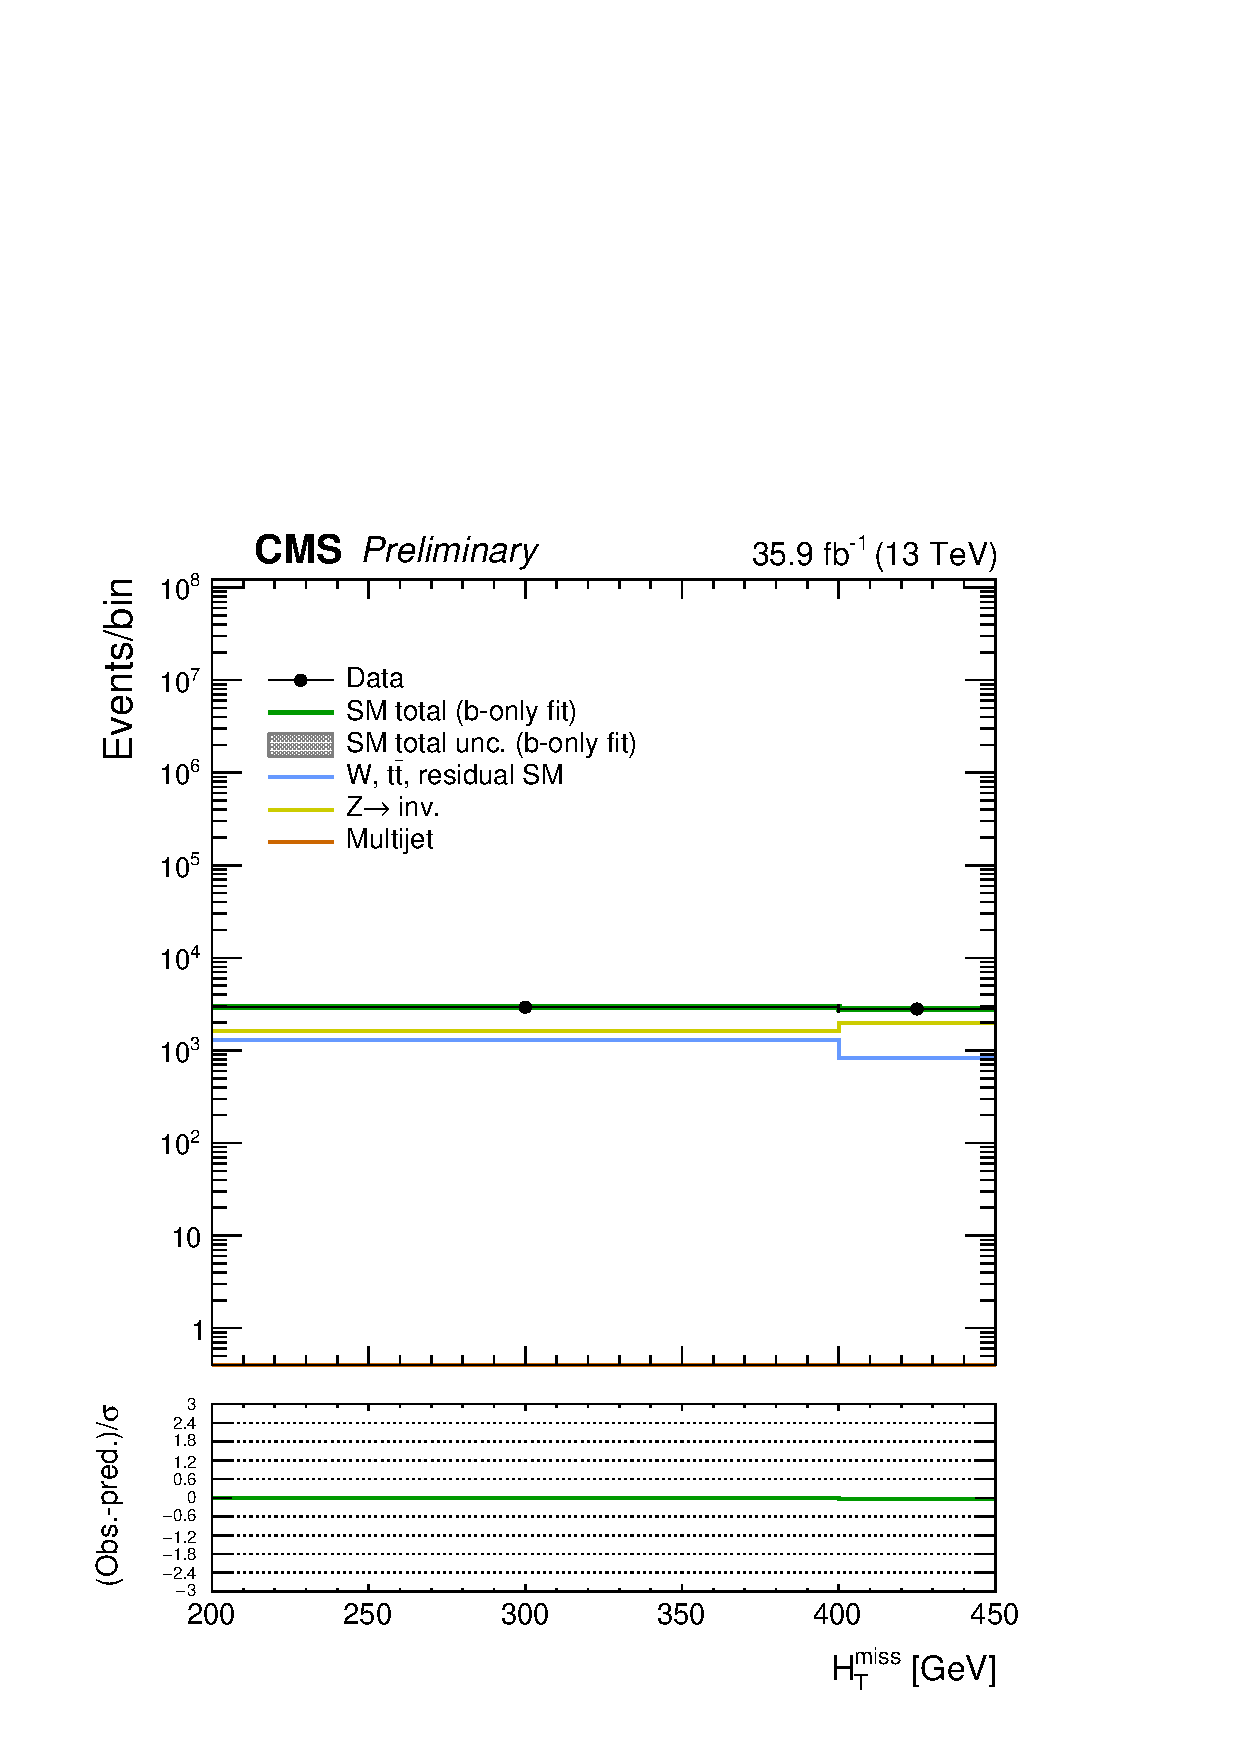
\includegraphics[width=0.49\textwidth]{figures/results/36invfb//crfit/shapes//mhtShape_eq0b_ge2a_400_600_fit_b.pdf}}
    \subfigure[$600 < \scalht < 900\GeV$]{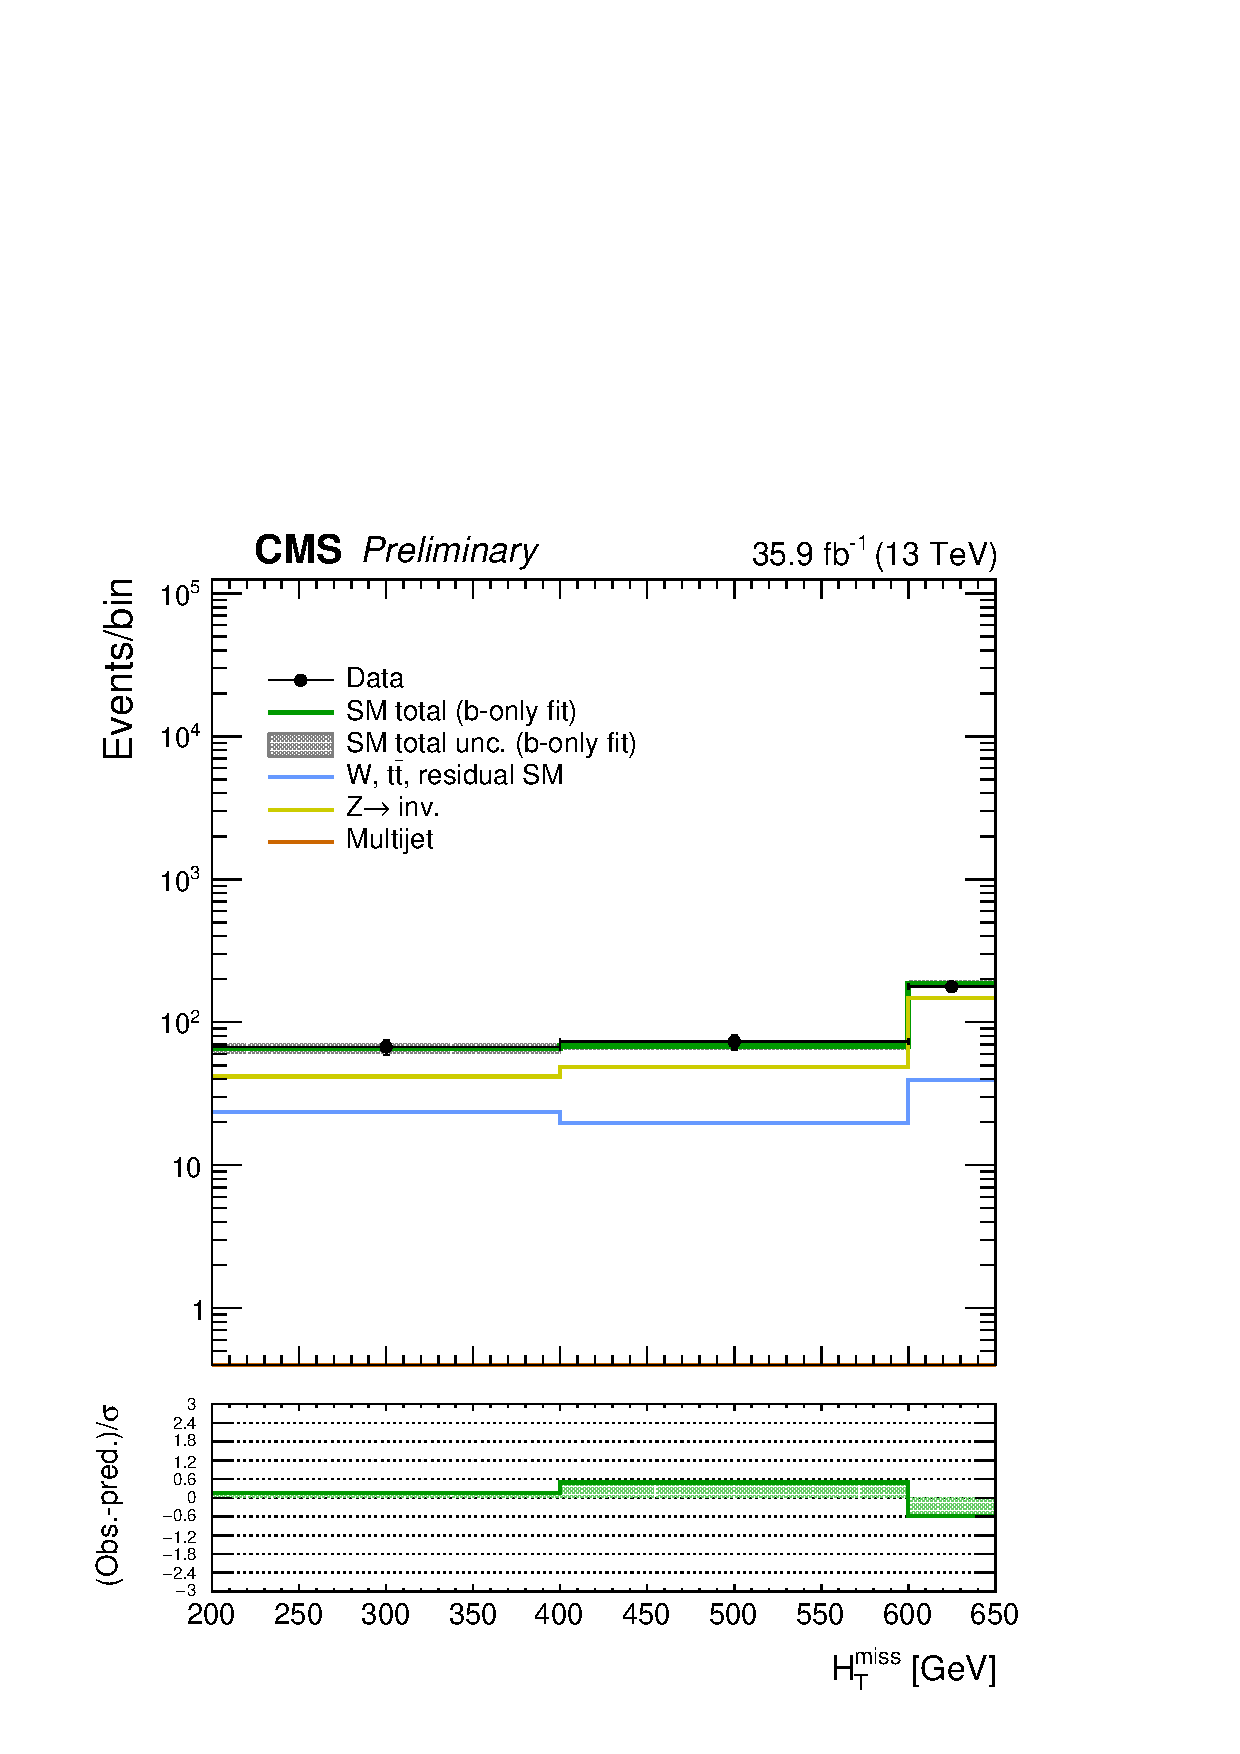
\includegraphics[width=0.49\textwidth]{figures/results/36invfb//crfit/shapes//mhtShape_eq0b_ge2a_600_900_fit_b.pdf}}\\
    \subfigure[$\scalht > 900\GeV$]{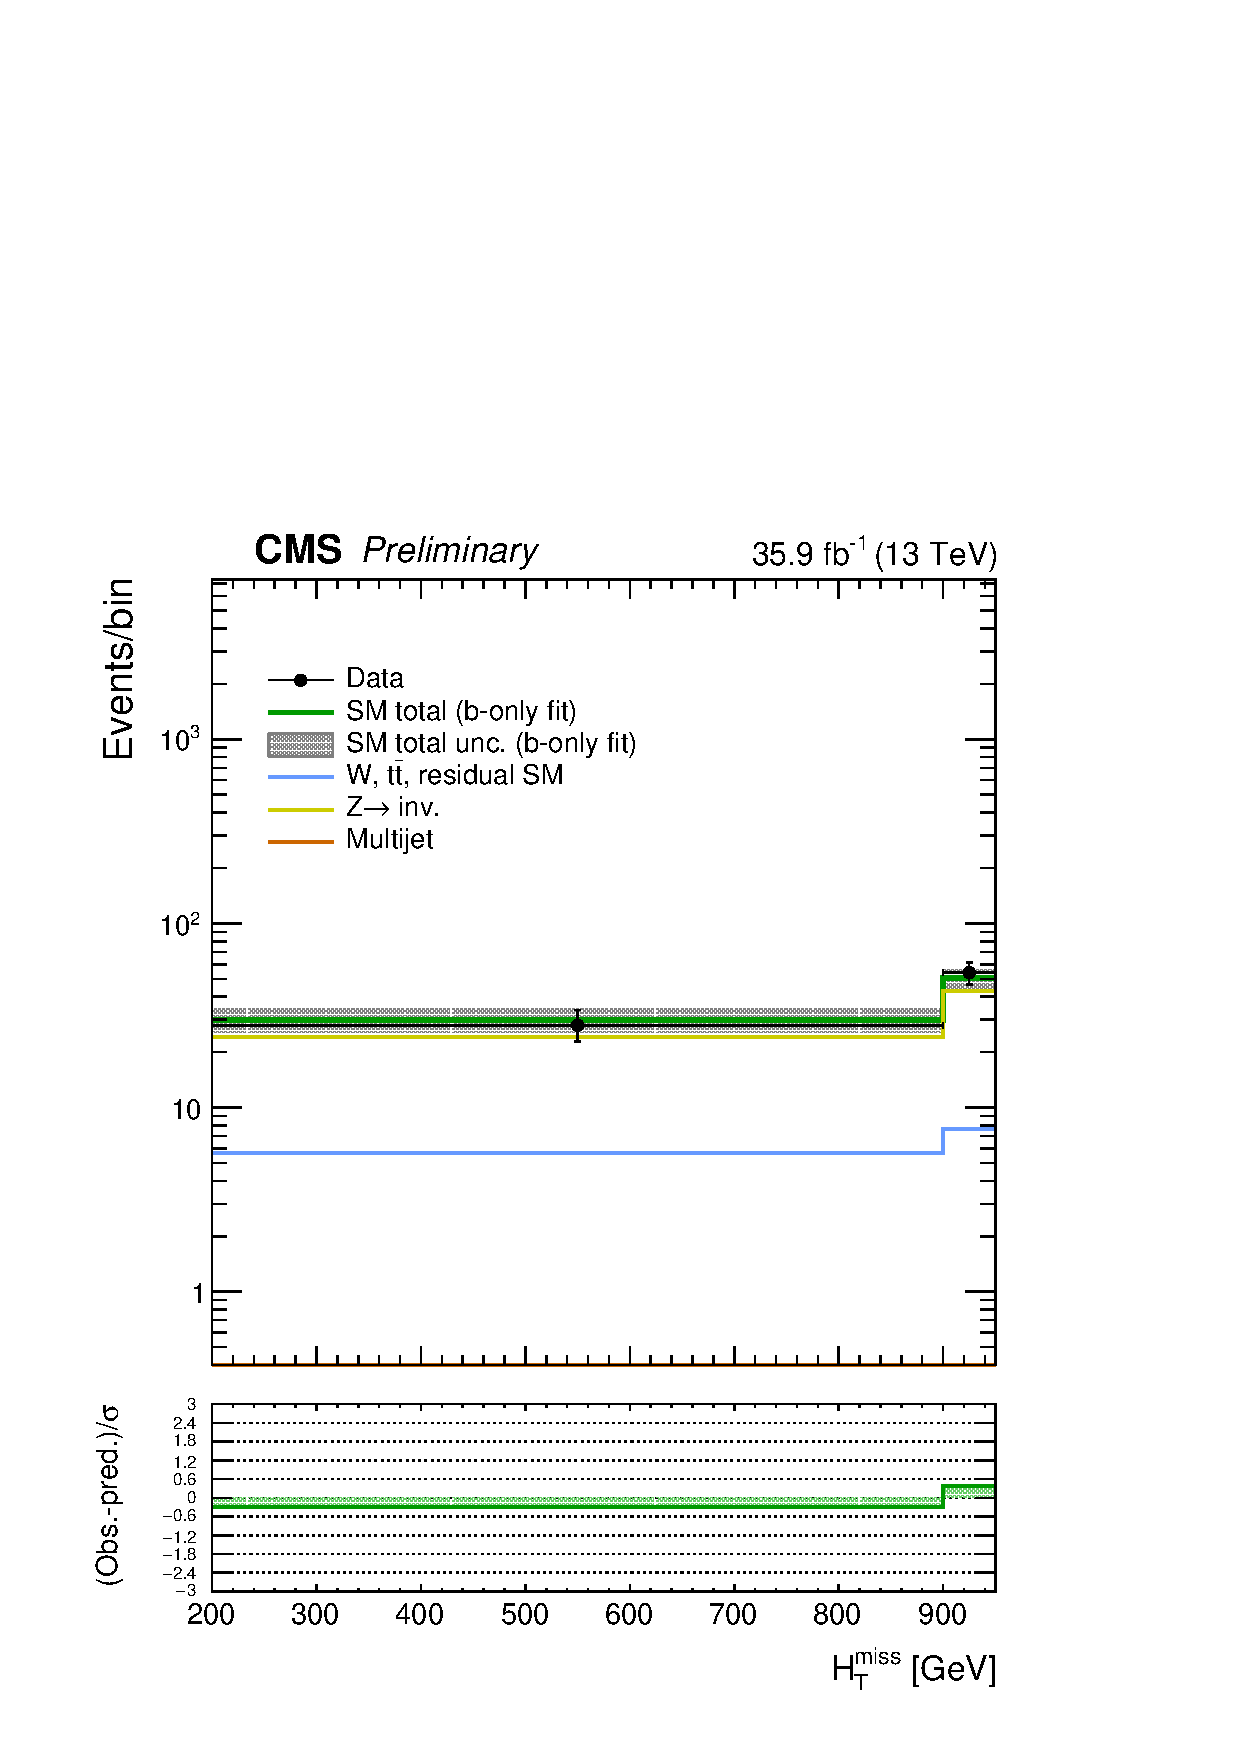
\includegraphics[width=0.49\textwidth]{figures/results/36invfb//crfit/shapes//mhtShape_eq0b_ge2a_900_Inf_fit_b.pdf}}
    \caption{Event yields observed in data (solid circles) and CR-fit SM expectations with their associated uncertainties (green histogram with shaded band) as a function of \HTmiss based on a sample of events that satisfy $\njet \geq 2 \; \textrm{(asymmetric)}$ and $\nb = 0$, as well as the requirements on \scalht indicated by each sub-figure caption. }
    \label{fig:mhtval_ge2a_eq0b}
  \end{center}
\end{figure}

\begin{figure}[h!]
  \begin{center}
    \subfigure[$400 < \scalht < 600\GeV$]{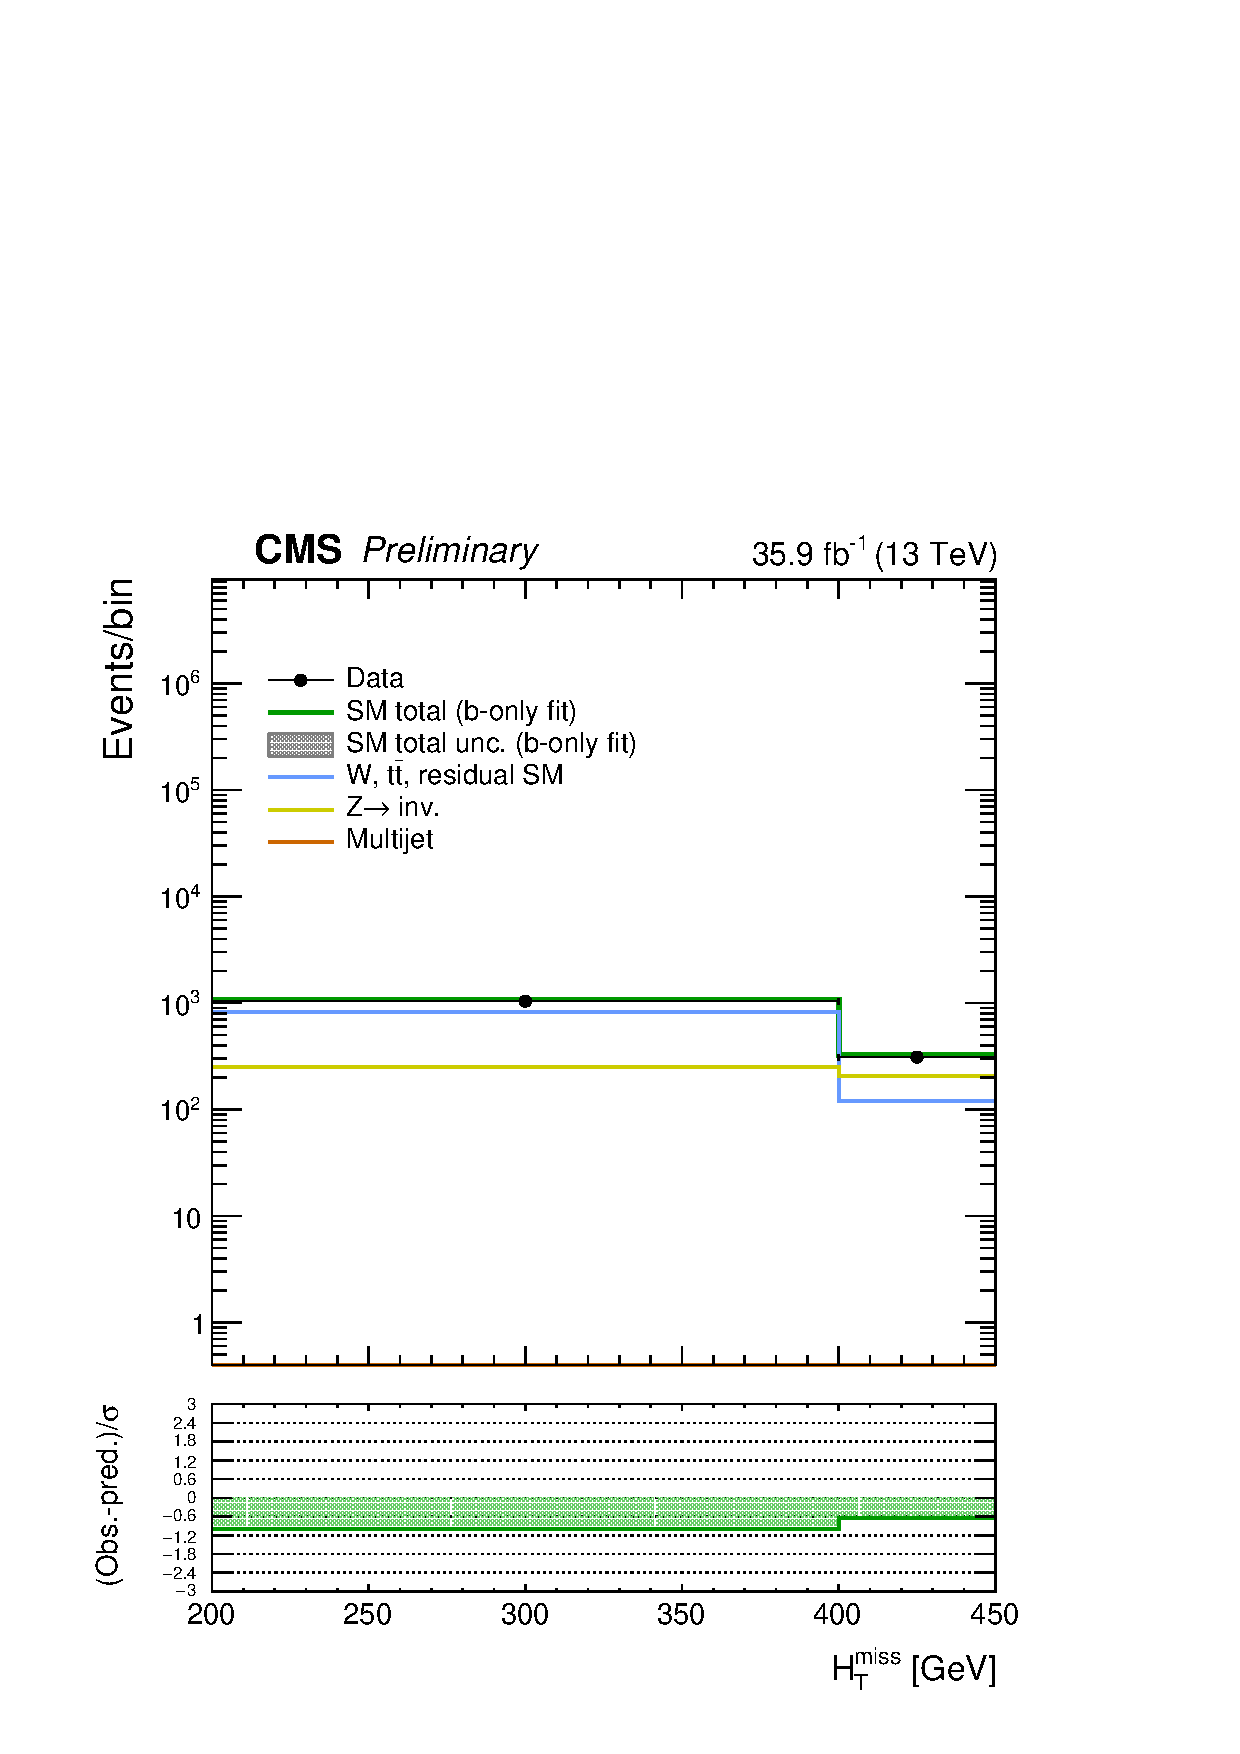
\includegraphics[width=0.49\textwidth]{figures/results/36invfb//crfit/shapes//mhtShape_eq1b_ge2a_400_600_fit_b.pdf}}
    \subfigure[$600 < \scalht < 900\GeV$]{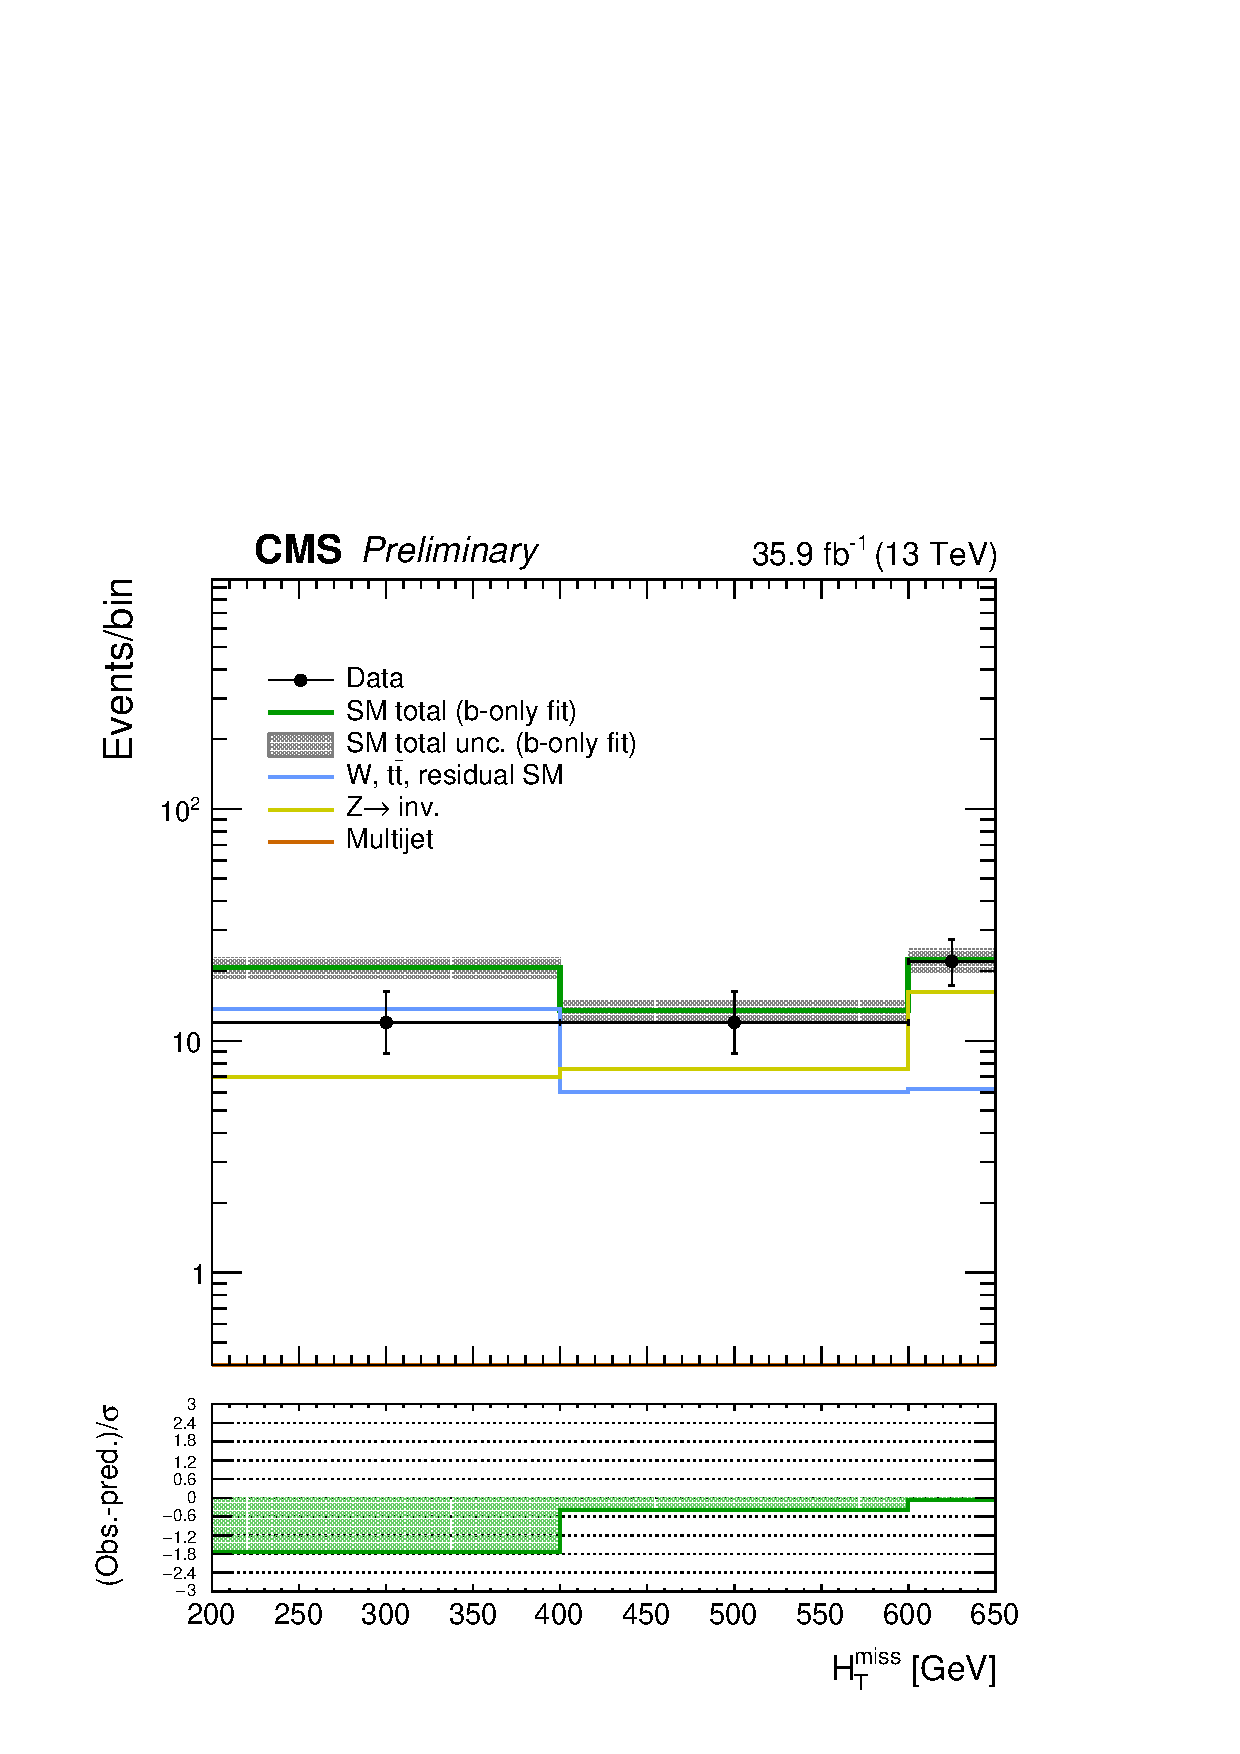
\includegraphics[width=0.49\textwidth]{figures/results/36invfb//crfit/shapes//mhtShape_eq1b_ge2a_600_900_fit_b.pdf}}\\
    \subfigure[$\scalht > 900\GeV$]{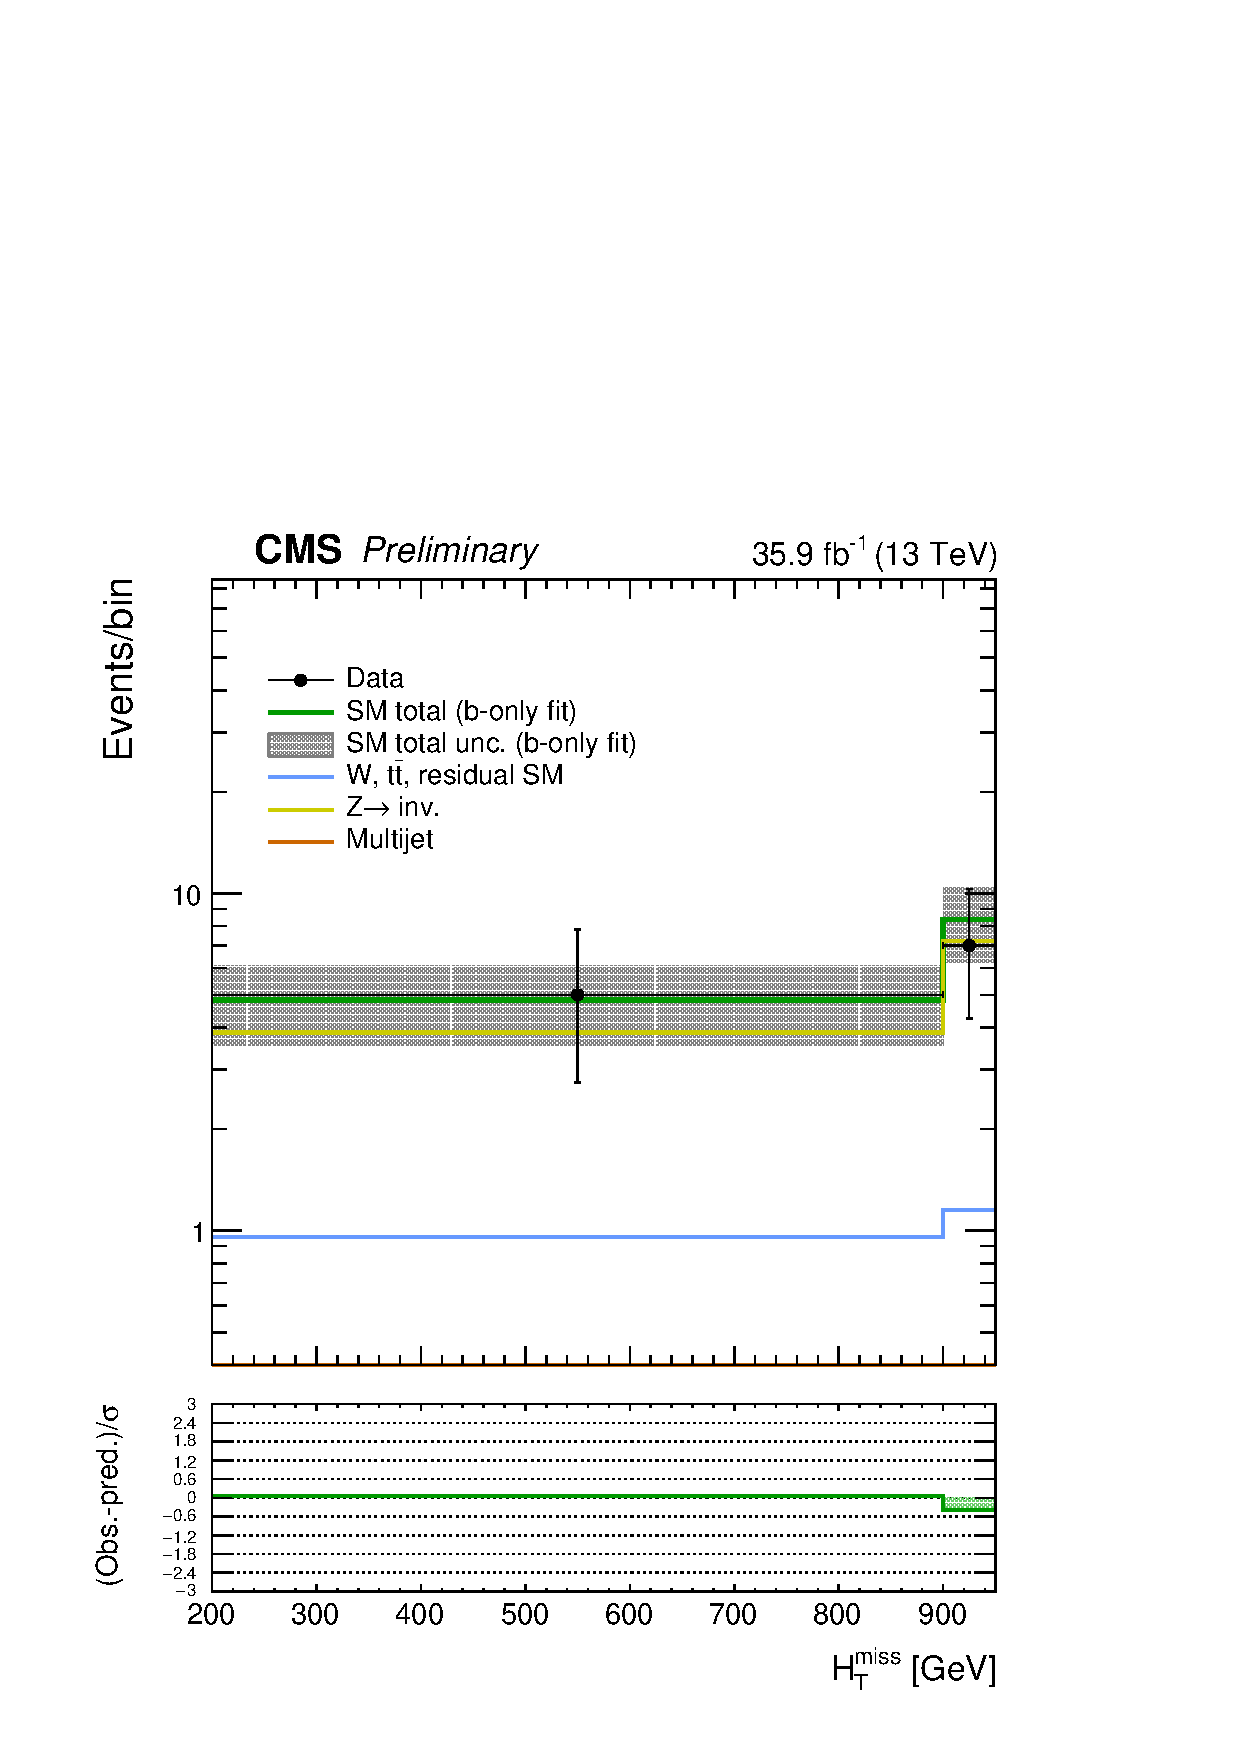
\includegraphics[width=0.49\textwidth]{figures/results/36invfb//crfit/shapes//mhtShape_eq1b_ge2a_900_Inf_fit_b.pdf}}
    \caption{Event yields observed in data (solid circles) and CR-fit SM expectations with their associated uncertainties (green histogram with shaded band) as a function of \HTmiss based on a sample of events that satisfy $\njet \geq 2 \; \textrm{(asymmetric)}$ and $\nb = 1$, as well as the requirements on \scalht indicated by each sub-figure caption. }
    \label{fig:mhtval_ge2a_eq1b}
  \end{center}
\end{figure}

\begin{figure}[h!]
  \begin{center}
    \subfigure[$400 < \scalht < 600\GeV$]{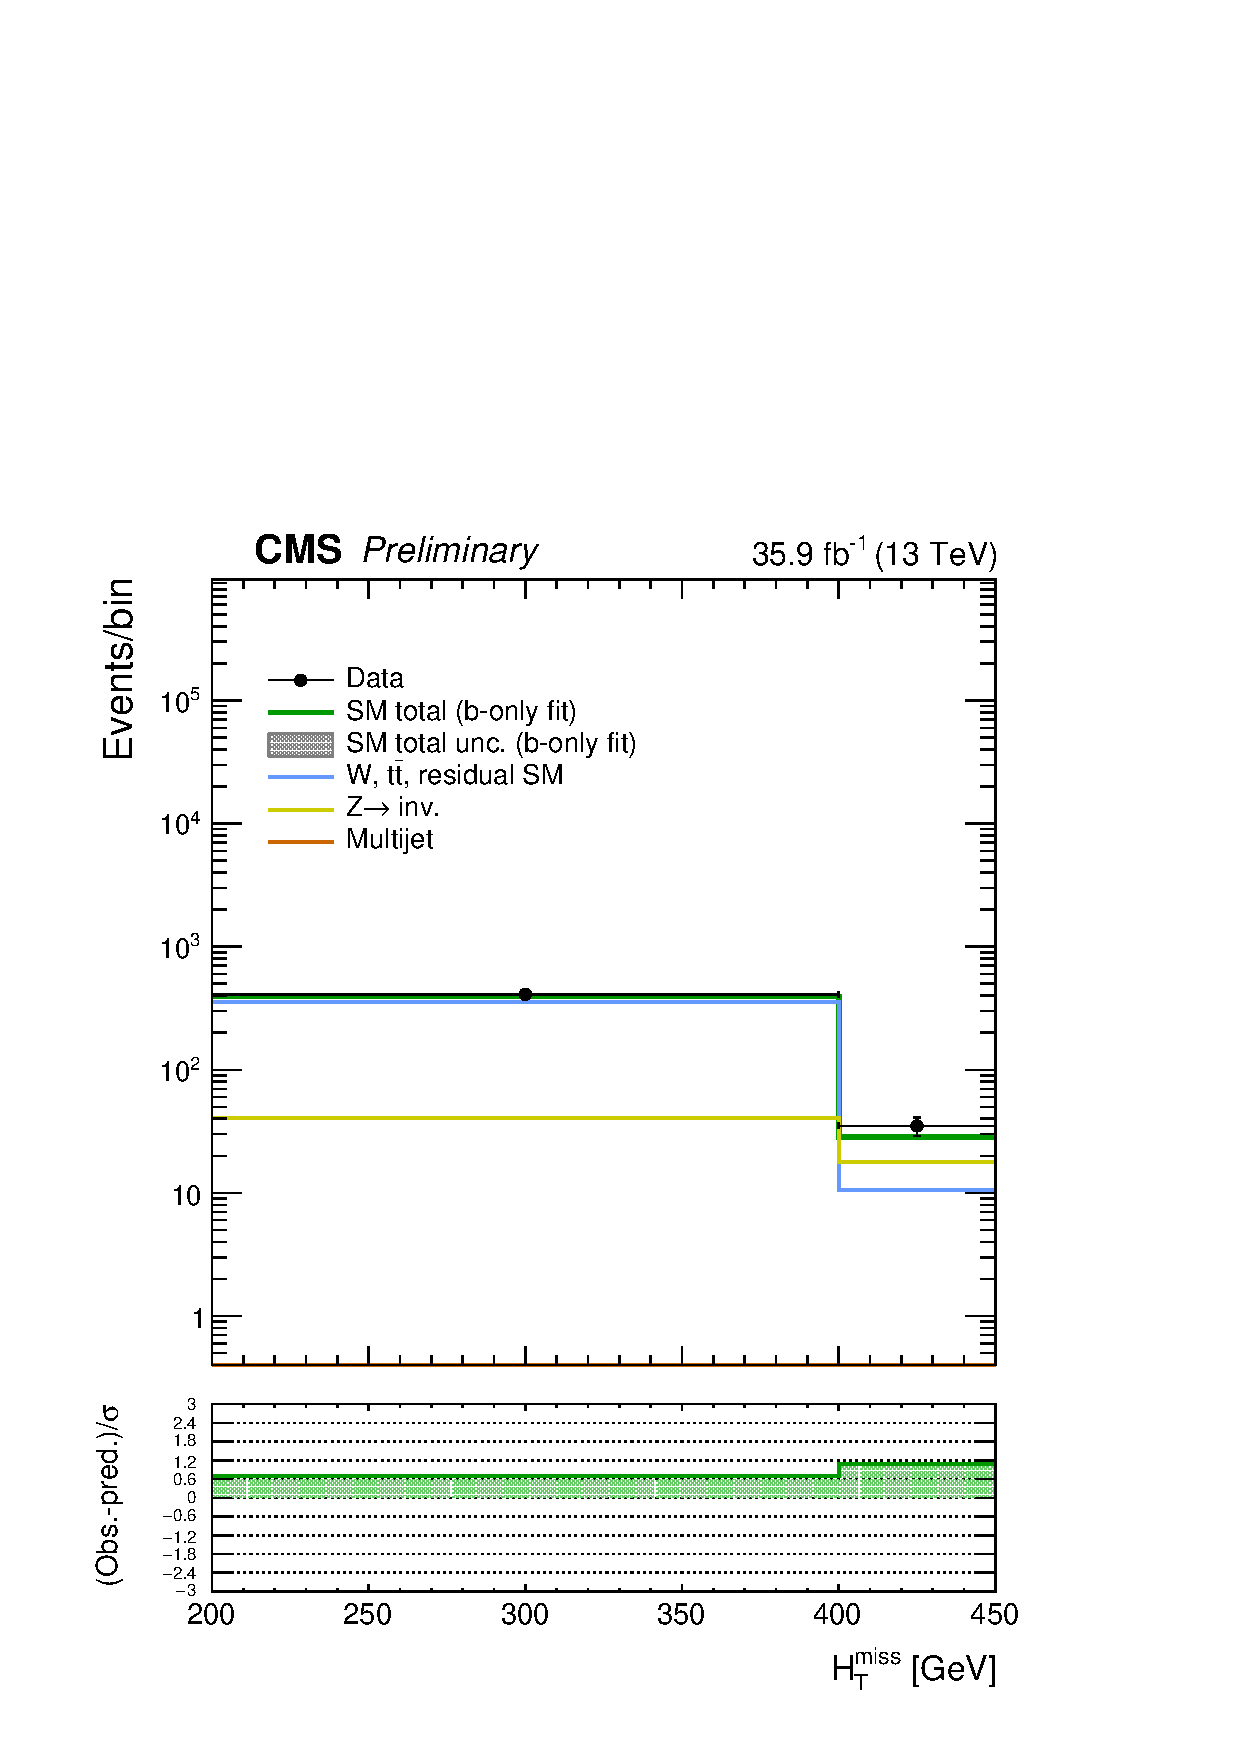
\includegraphics[width=0.49\textwidth]{figures/results/36invfb//crfit/shapes//mhtShape_eq2b_ge2a_400_600_fit_b.pdf}}
    \subfigure[$600 < \scalht < 900\GeV$]{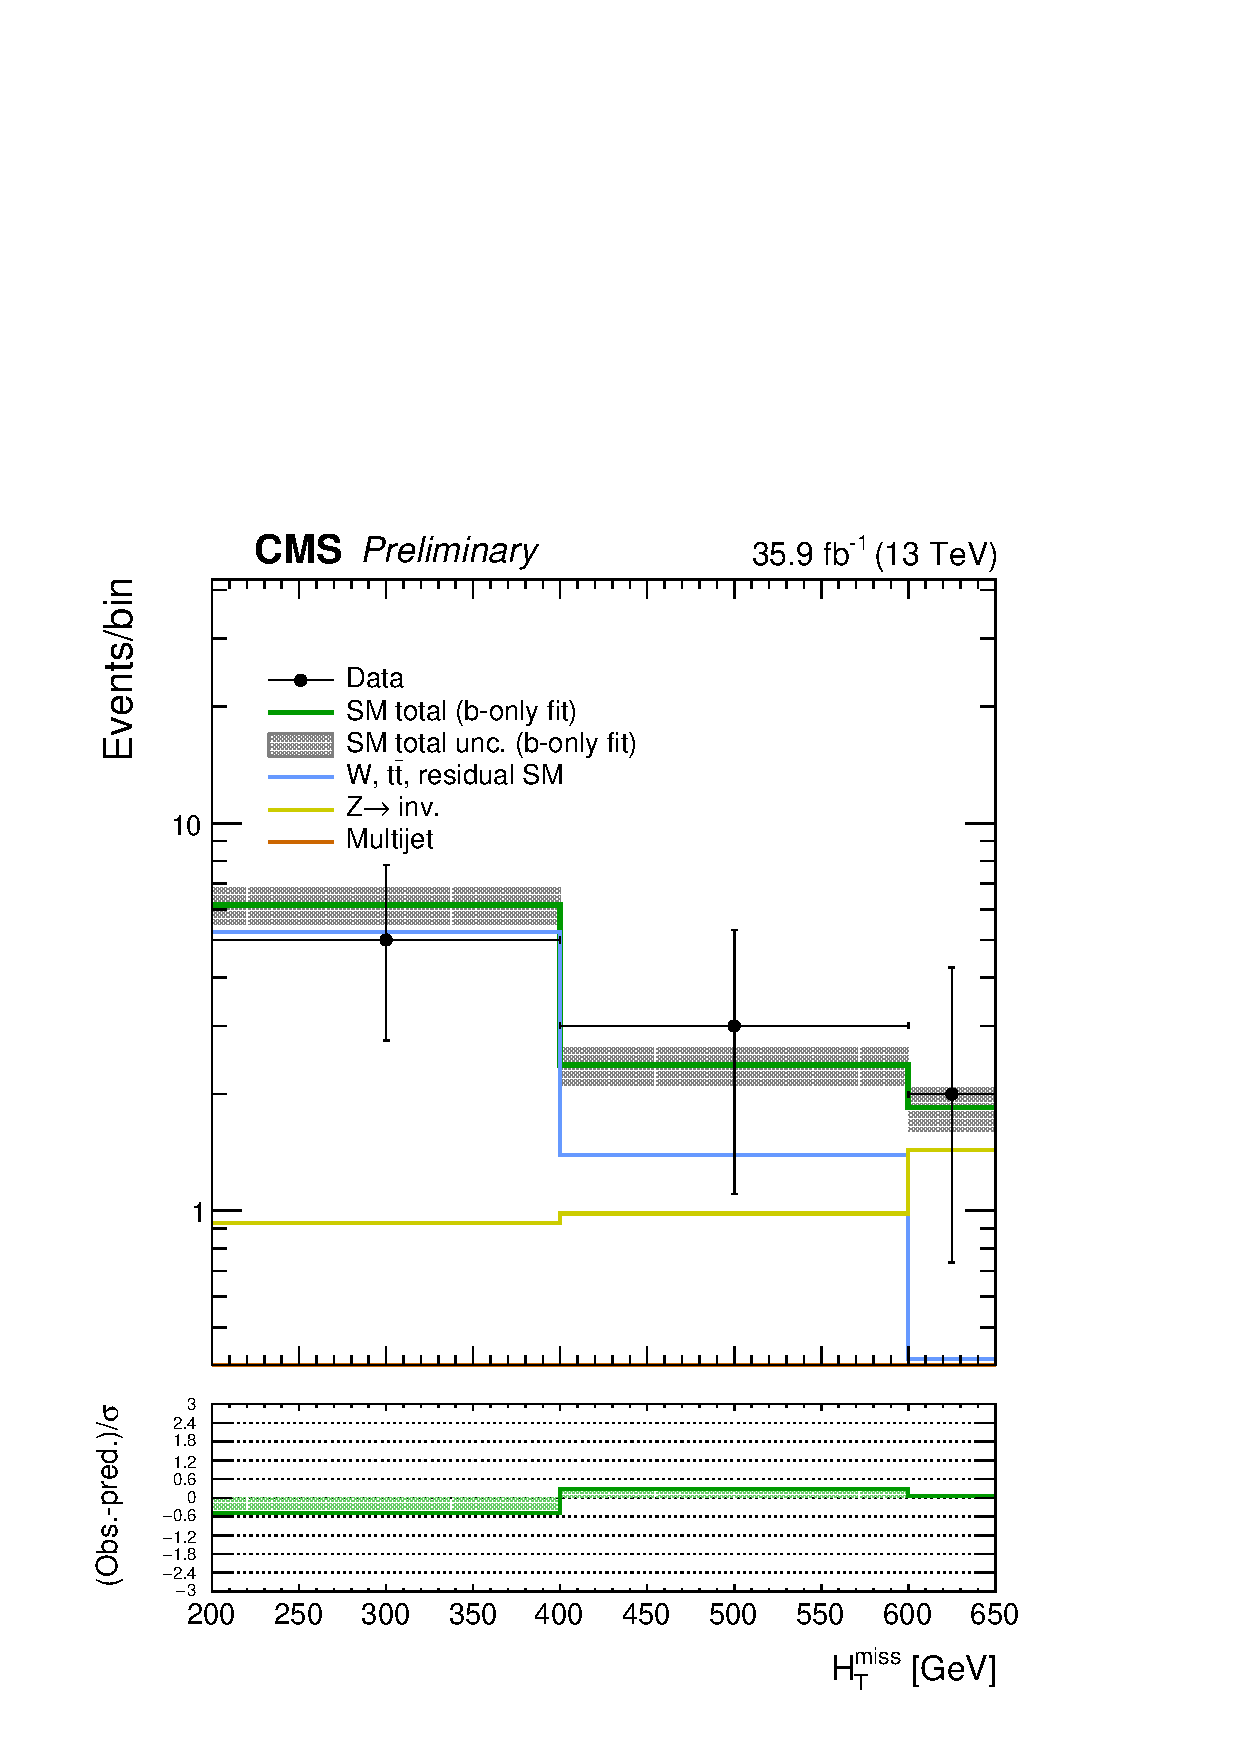
\includegraphics[width=0.49\textwidth]{figures/results/36invfb//crfit/shapes//mhtShape_eq2b_ge2a_600_900_fit_b.pdf}}\\
    \subfigure[$\scalht > 900\GeV$]{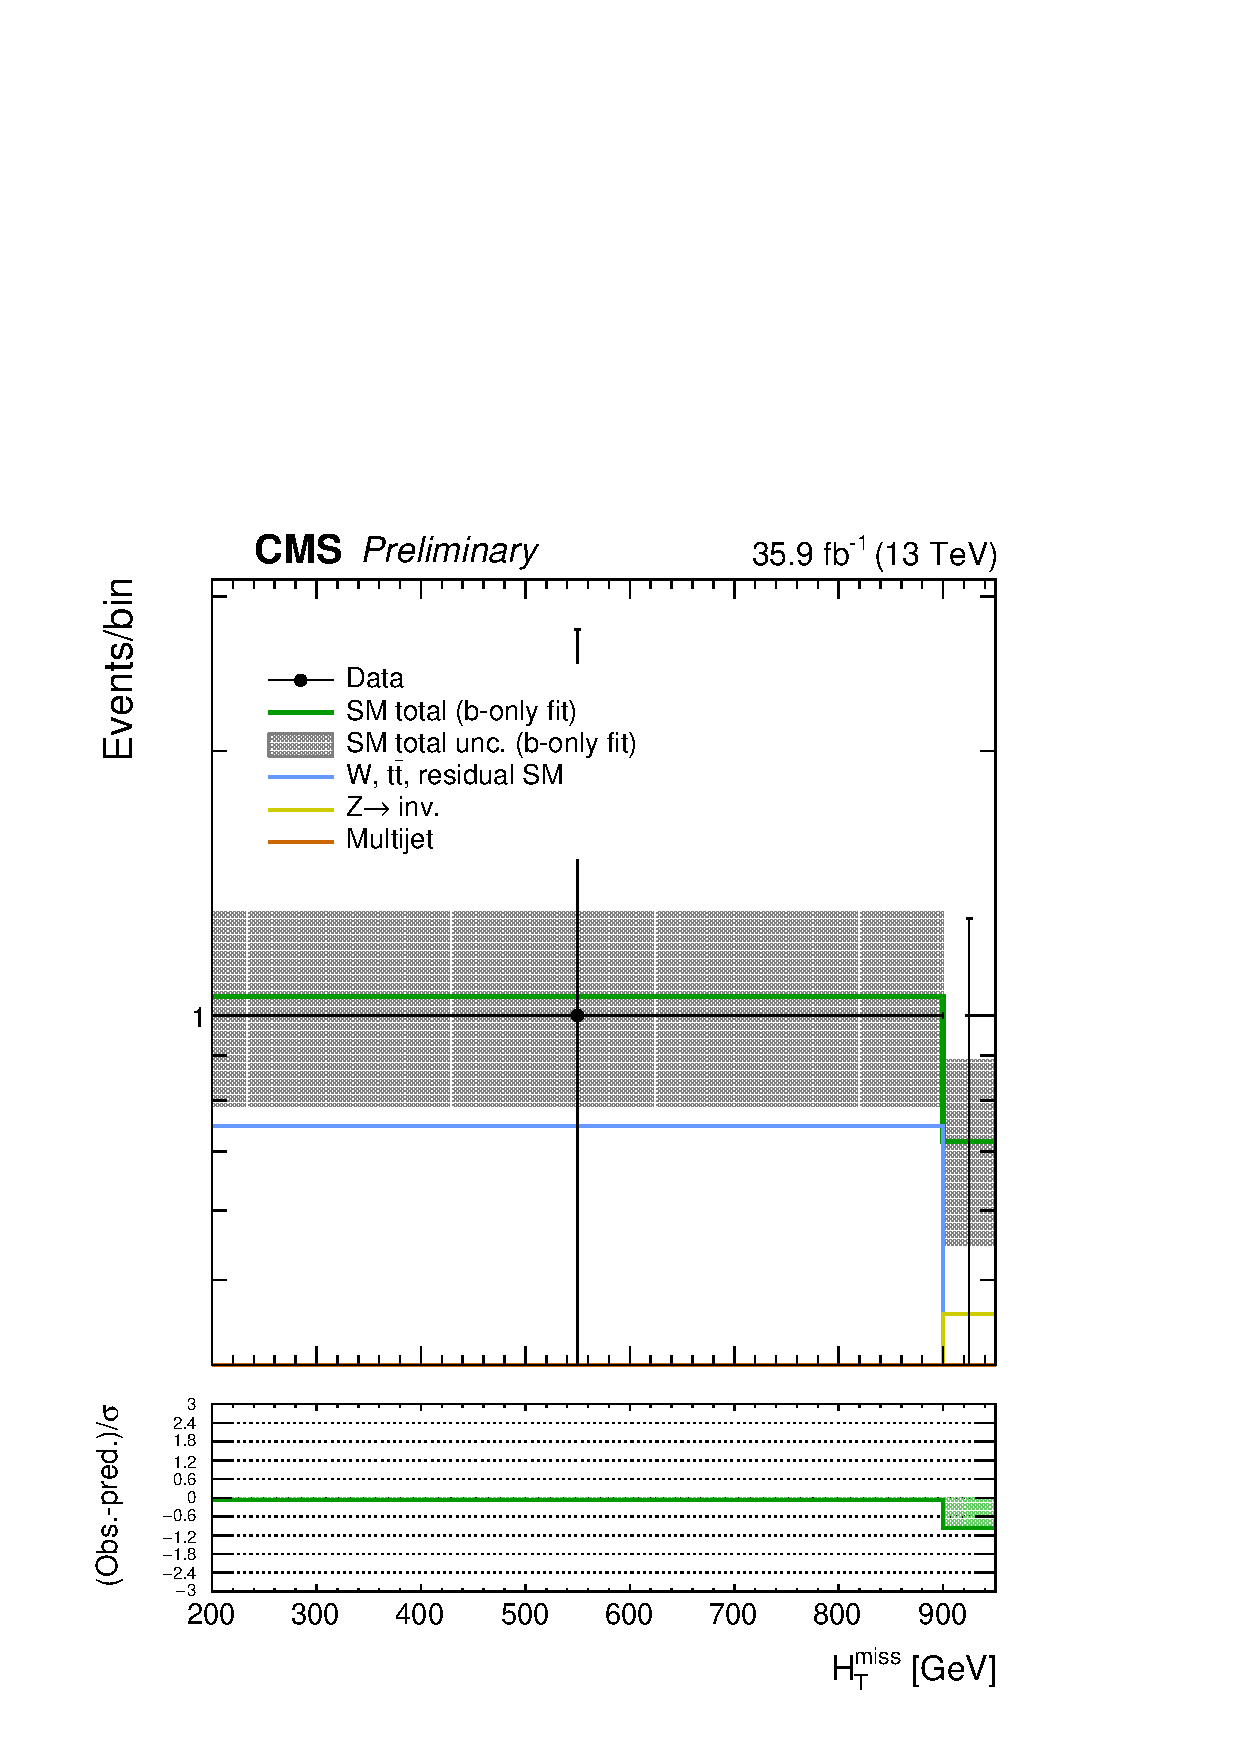
\includegraphics[width=0.49\textwidth]{figures/results/36invfb//crfit/shapes//mhtShape_eq2b_ge2a_900_Inf_fit_b.pdf}}
    \caption{Event yields observed in data (solid circles) and CR-fit SM expectations with their associated uncertainties (green histogram with shaded band) as a function of \HTmiss based on a sample of events that satisfy $\njet \geq 2 \; \textrm{(asymmetric)}$ and $\nb = 2$, as well as the requirements on \scalht indicated by each sub-figure caption. }
    \label{fig:mhtval_ge2a_eq2b}
  \end{center}
\end{figure}

\begin{figure}[h!]
  \begin{center}
    \subfigure[$400 < \scalht < 600\GeV$]{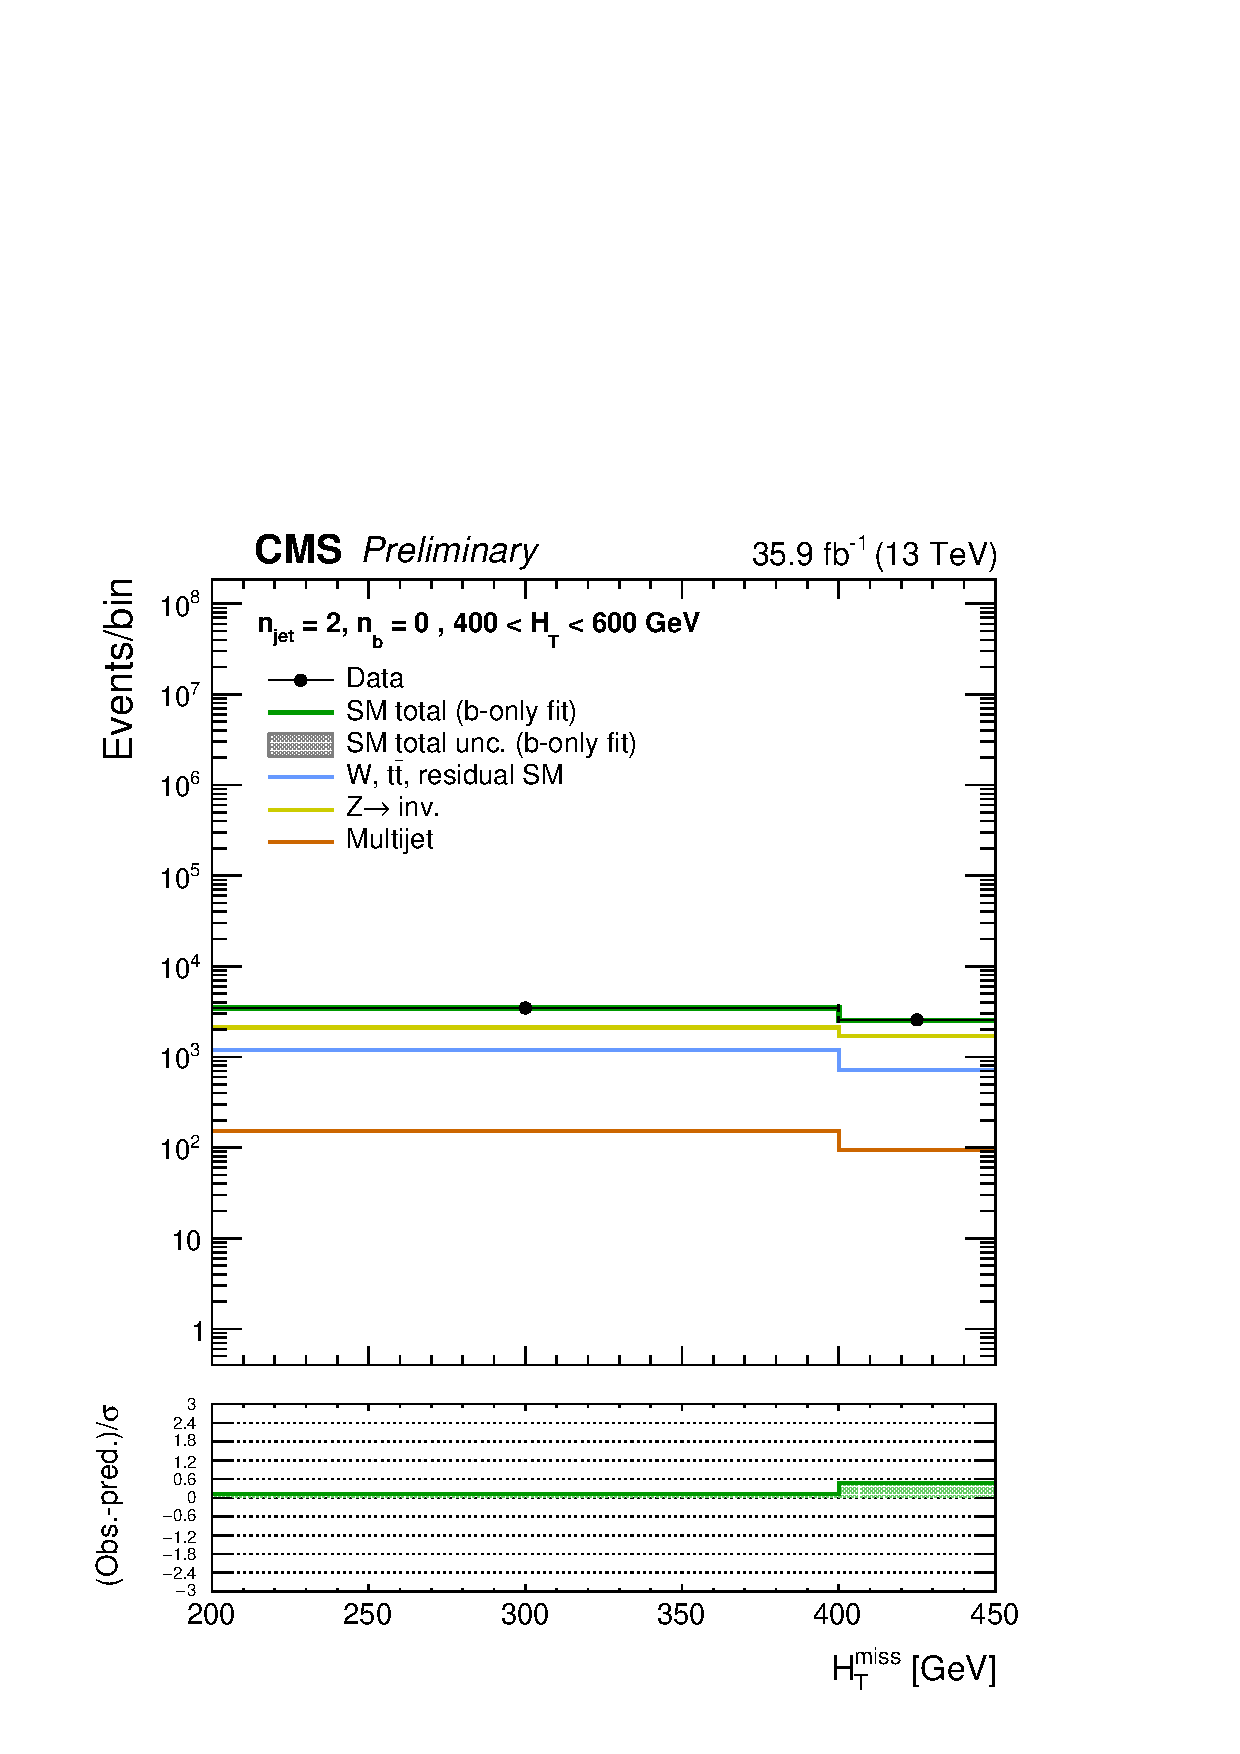
\includegraphics[width=0.49\textwidth]{figures/results/36invfb//crfit/shapes//mhtShape_eq0b_eq2j_400_600_fit_b.pdf}}
    \subfigure[$600 < \scalht < 900\GeV$]{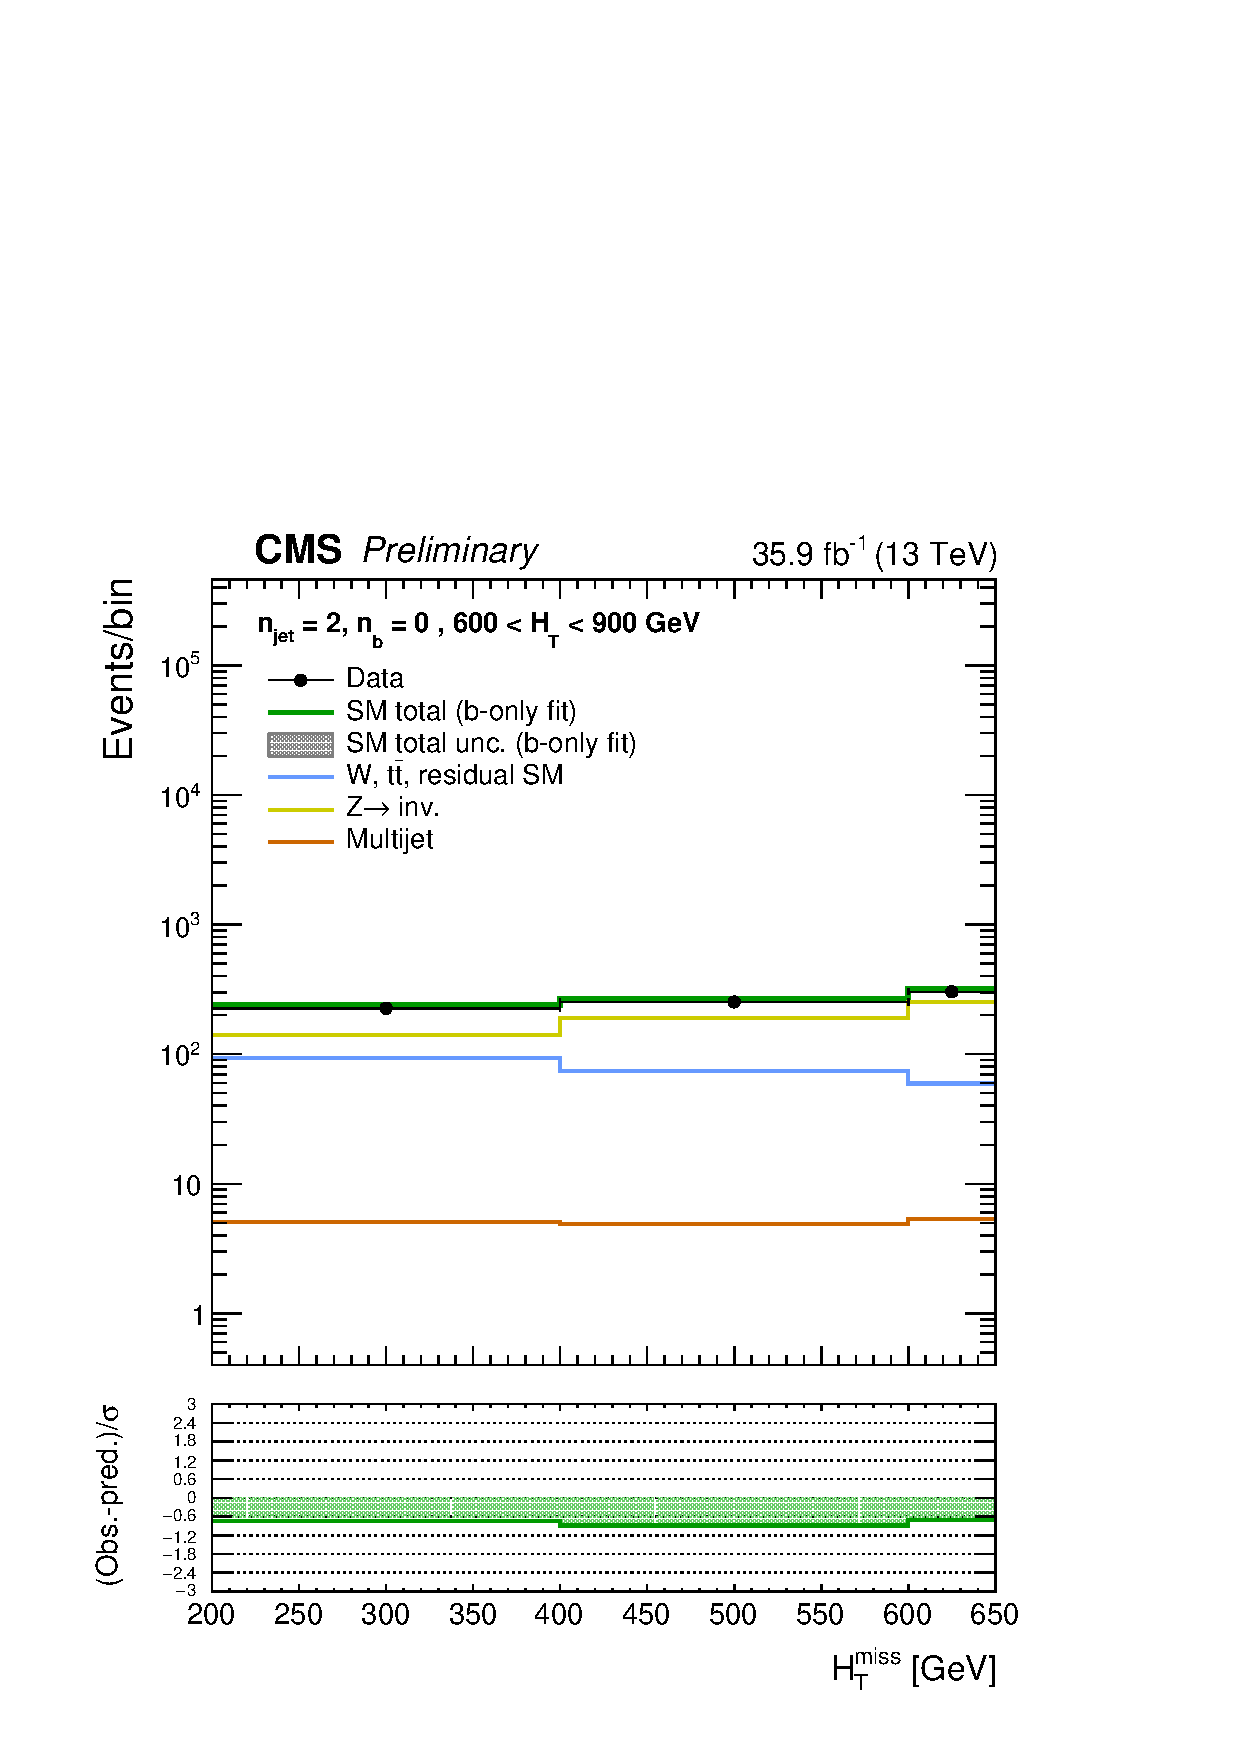
\includegraphics[width=0.49\textwidth]{figures/results/36invfb//crfit/shapes//mhtShape_eq0b_eq2j_600_900_fit_b.pdf}}\\
    \subfigure[$900 < \scalht < 1200\GeV$]{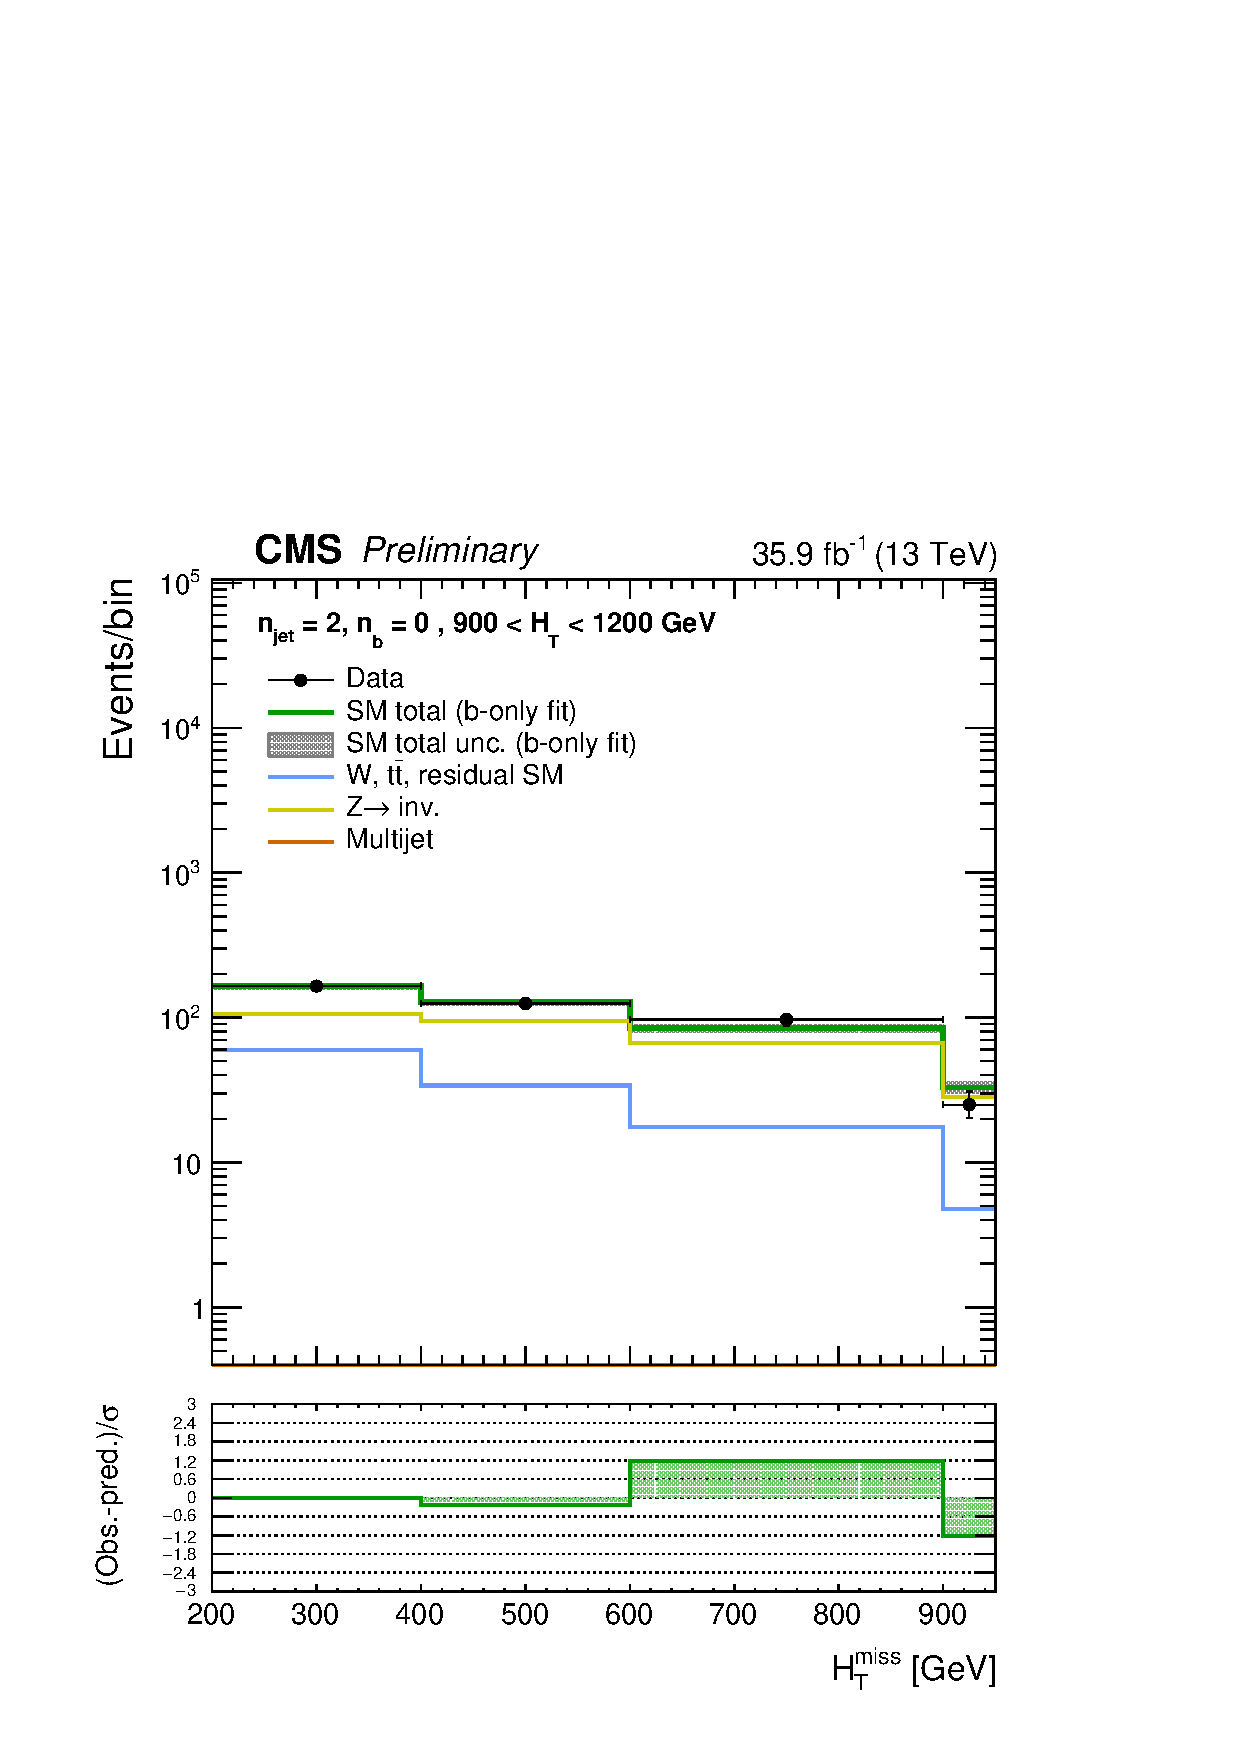
\includegraphics[width=0.49\textwidth]{figures/results/36invfb//crfit/shapes//mhtShape_eq0b_eq2j_900_1200_fit_b.pdf}}
    \subfigure[$\scalht > 1200\GeV$]{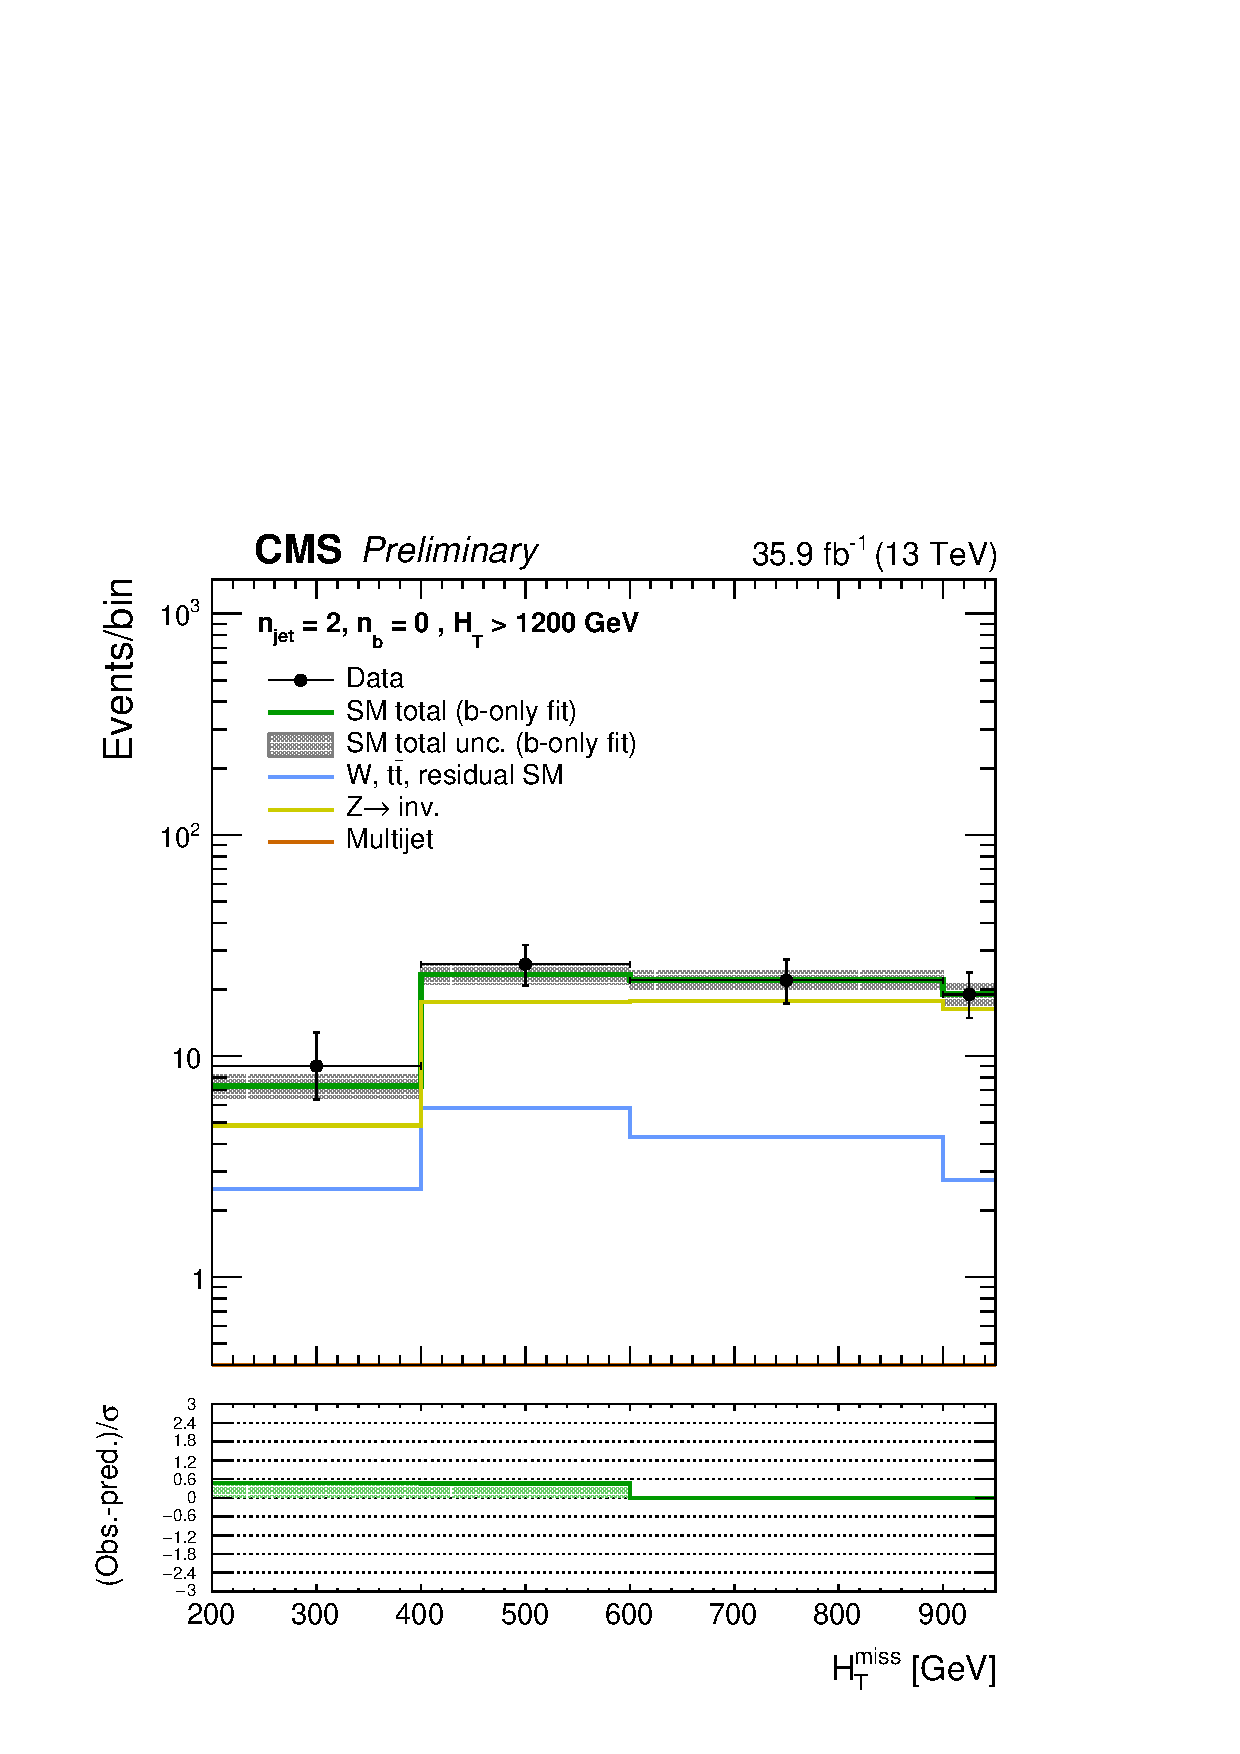
\includegraphics[width=0.49\textwidth]{figures/results/36invfb//crfit/shapes//mhtShape_eq0b_eq2j_1200_Inf_fit_b.pdf}}\\
    \caption{Event yields observed in data (solid circles) and CR-fit SM expectations with their associated uncertainties (green histogram with shaded band) as a function of \HTmiss based on a sample of events that satisfy $\njet = 2$ and $\nb = 0$, as well as the requirements on \scalht indicated by each sub-figure caption. }
    \label{fig:mhtval_eq2j_eq0b}
  \end{center}
\end{figure}

\begin{figure}[h!]
  \begin{center}
    \subfigure[$400 < \scalht < 600\GeV$]{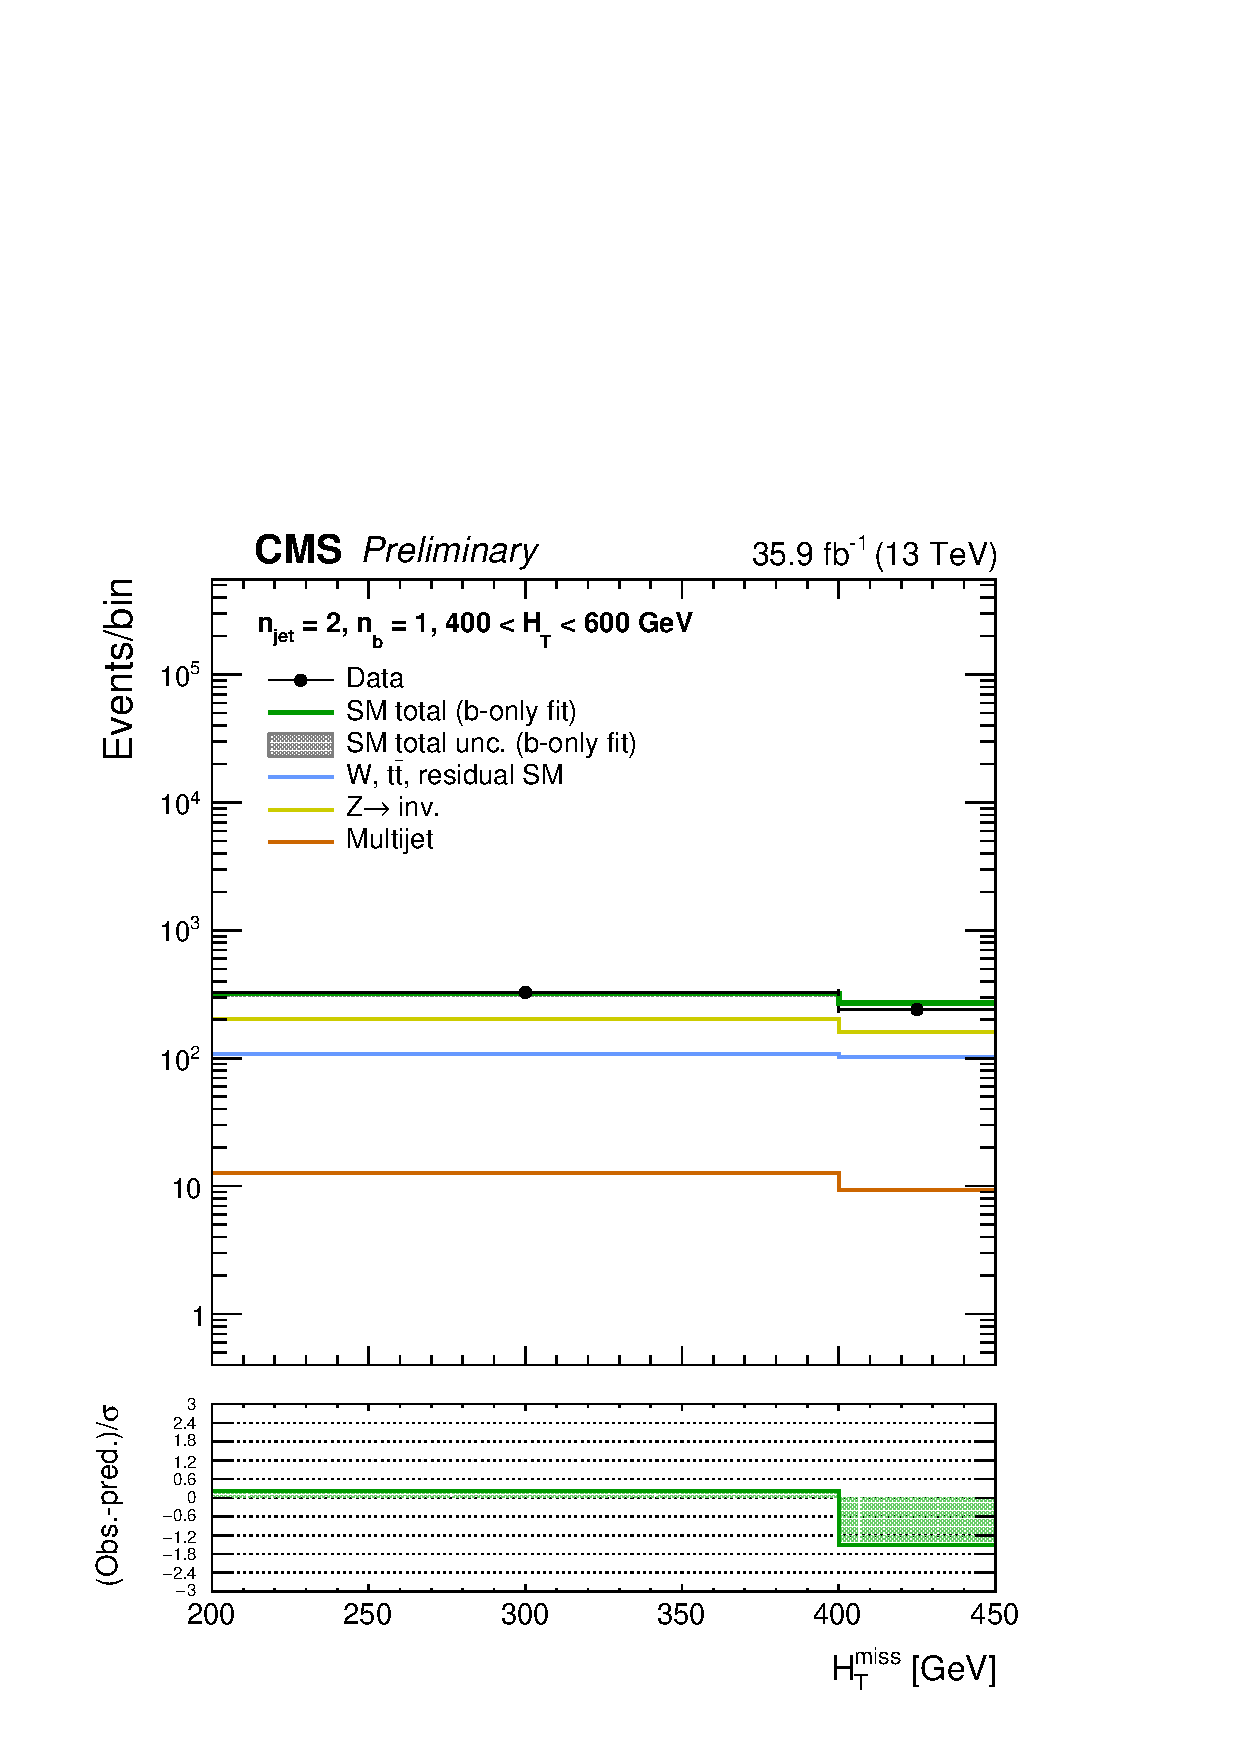
\includegraphics[width=0.49\textwidth]{figures/results/36invfb//crfit/shapes//mhtShape_eq1b_eq2j_400_600_fit_b.pdf}}
    \subfigure[$600 < \scalht < 900\GeV$]{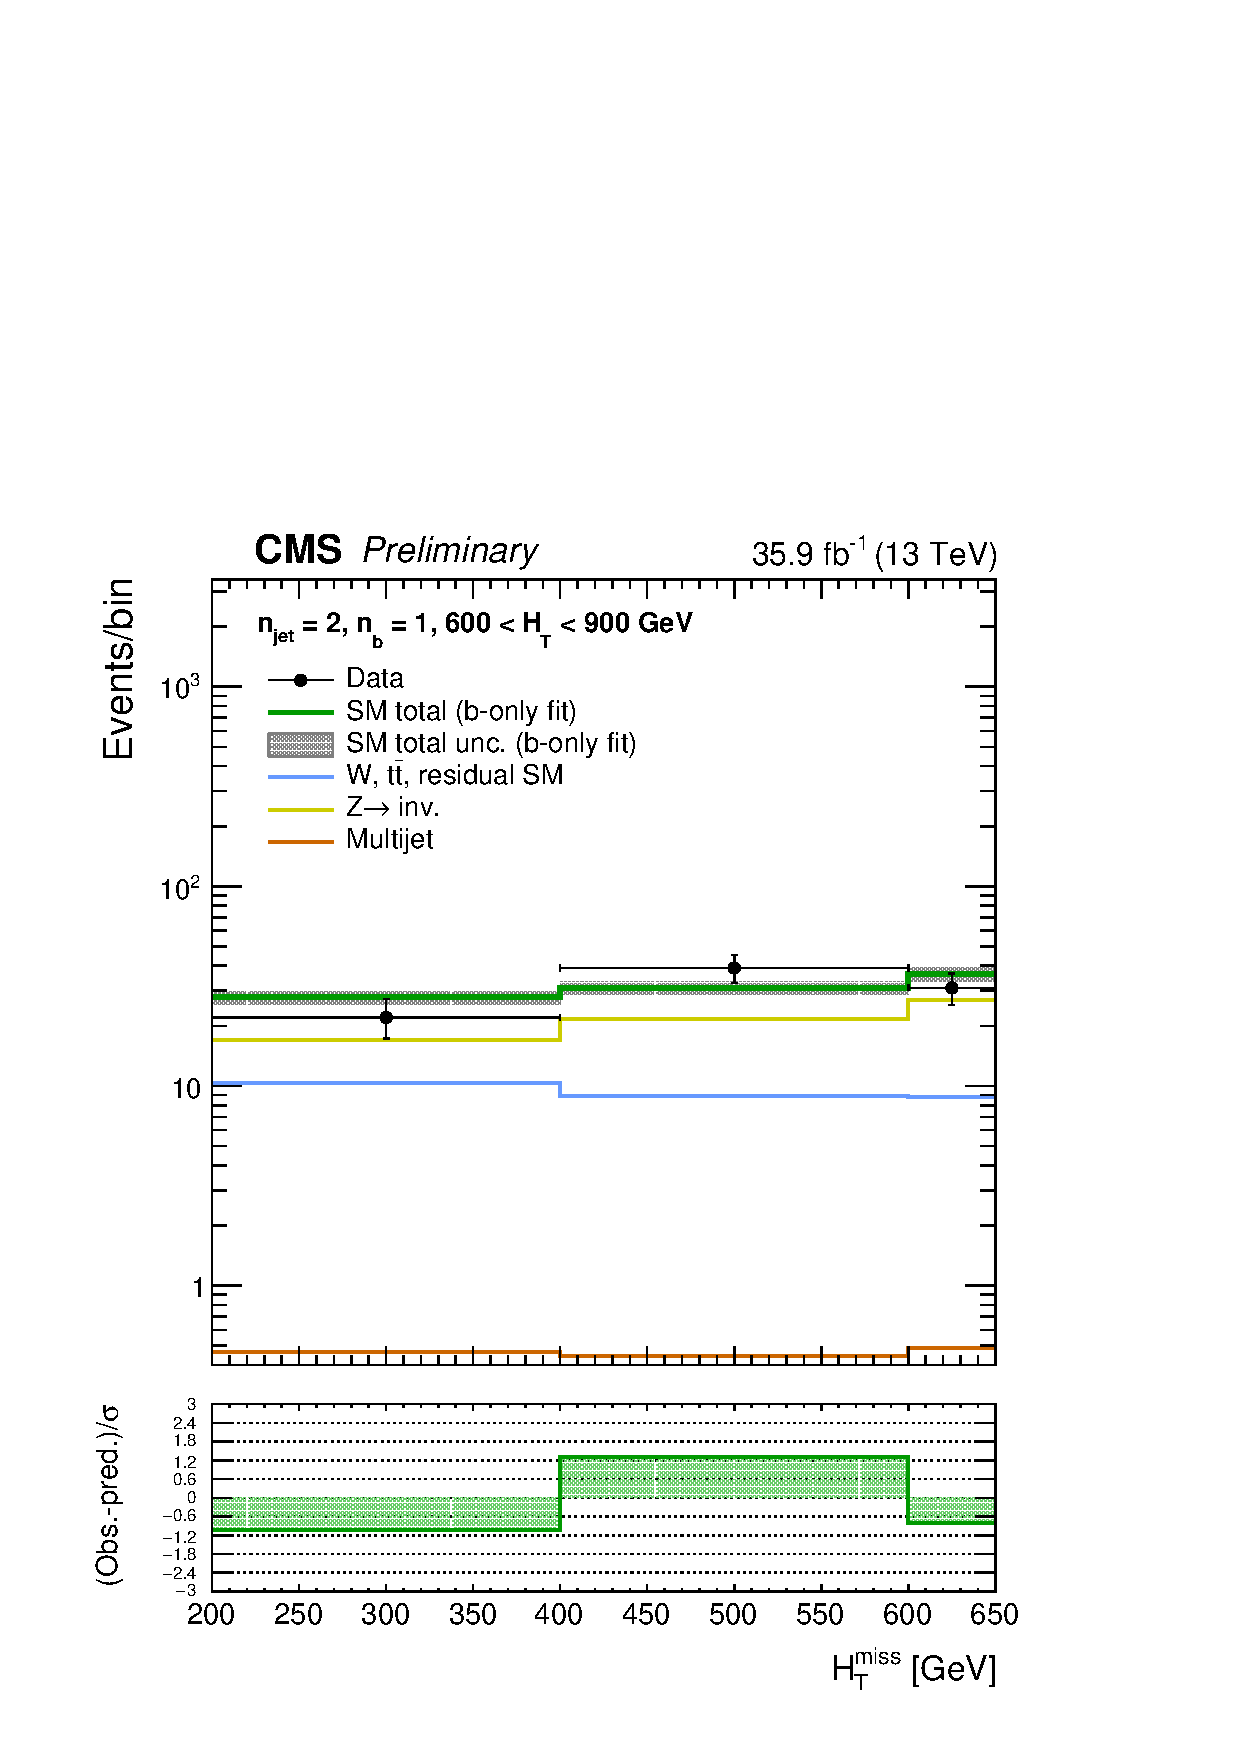
\includegraphics[width=0.49\textwidth]{figures/results/36invfb//crfit/shapes//mhtShape_eq1b_eq2j_600_900_fit_b.pdf}}\\
    \subfigure[$900 < \scalht < 1200\GeV$]{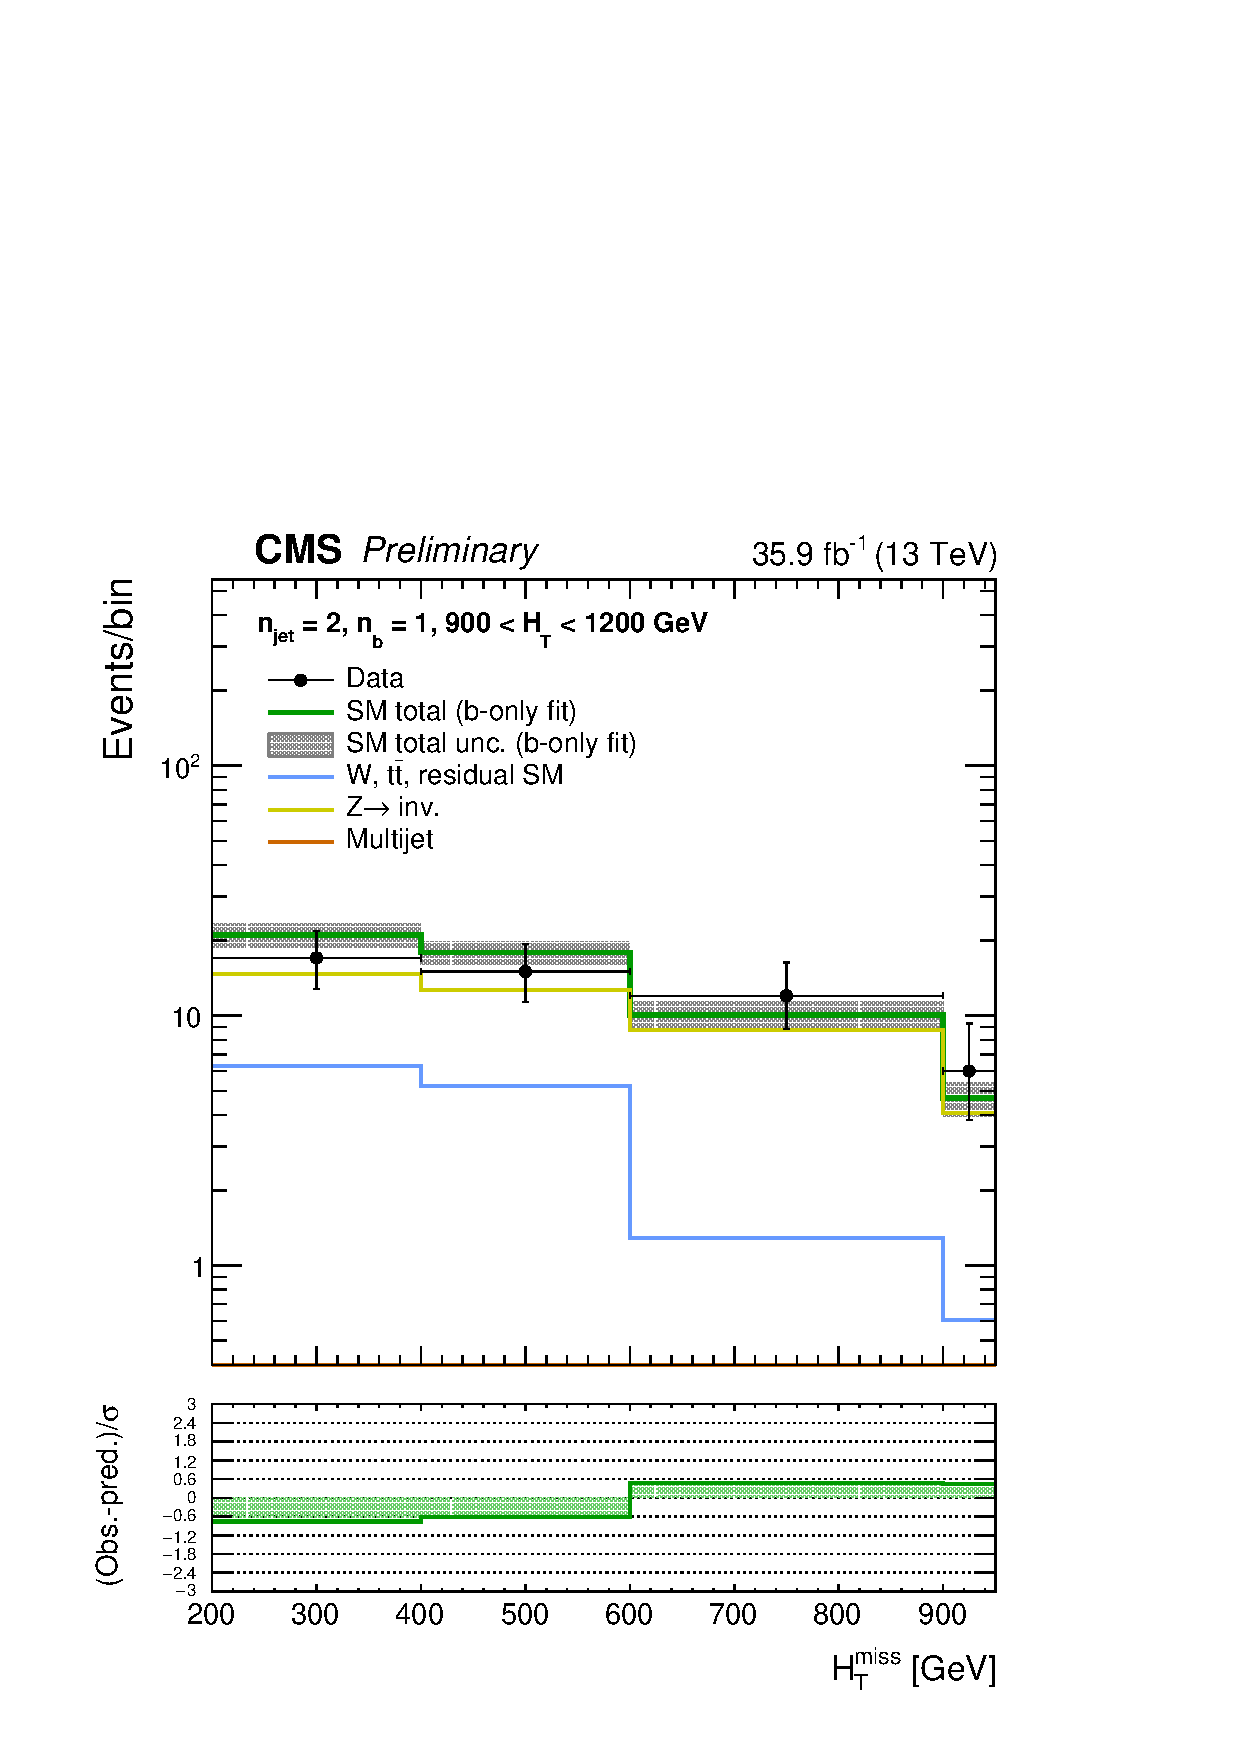
\includegraphics[width=0.49\textwidth]{figures/results/36invfb//crfit/shapes//mhtShape_eq1b_eq2j_900_1200_fit_b.pdf}}
    \subfigure[$\scalht > 1200\GeV$]{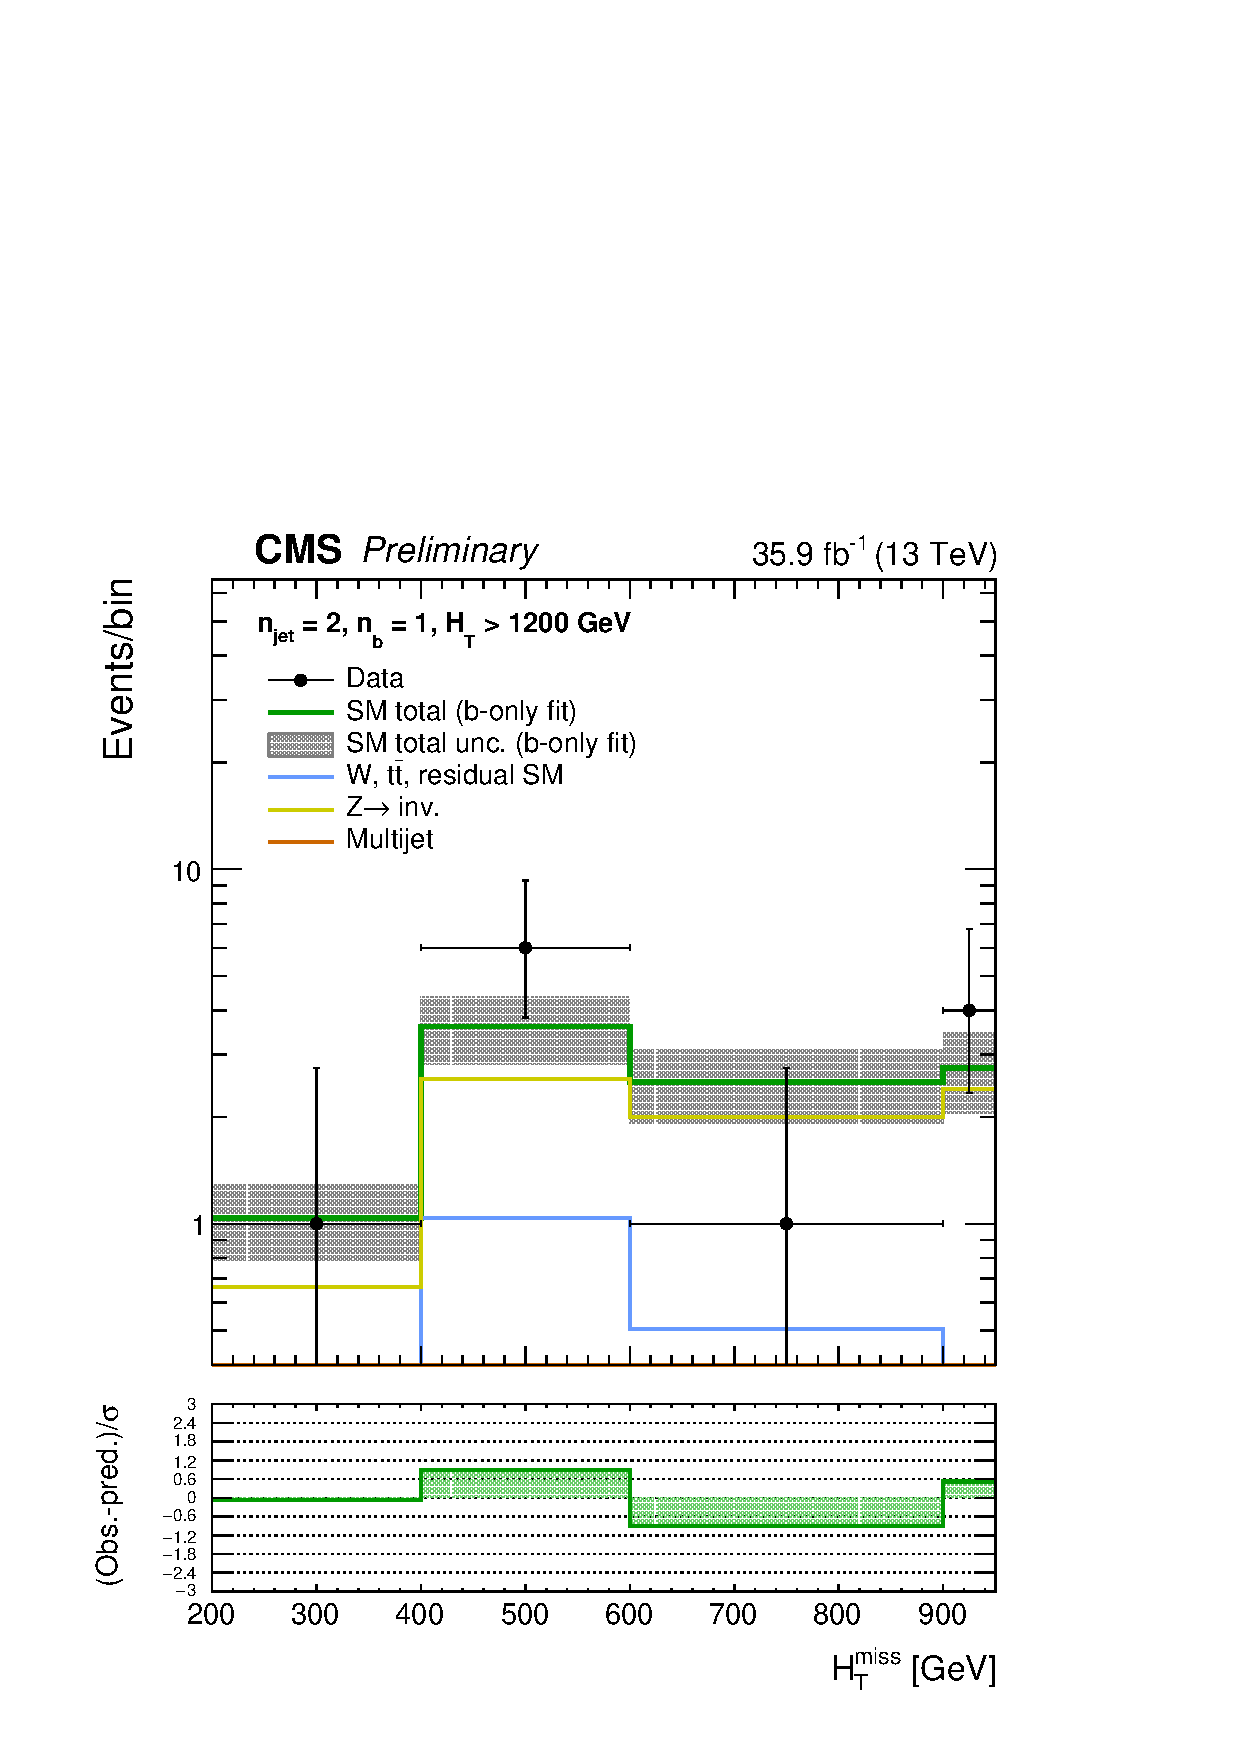
\includegraphics[width=0.49\textwidth]{figures/results/36invfb//crfit/shapes//mhtShape_eq1b_eq2j_1200_Inf_fit_b.pdf}}\\
    \caption{Event yields observed in data (solid circles) and CR-fit SM expectations with their associated uncertainties (green histogram with shaded band) as a function of \HTmiss based on a sample of events that satisfy $\njet = 2$ and $\nb = 1$, as well as the requirements on \scalht indicated by each sub-figure caption. }
    \label{fig:mhtval_eq2j_eq1b}
  \end{center}
\end{figure}

\begin{figure}[h!]
  \begin{center}
    \subfigure[$400 < \scalht < 600\GeV$]{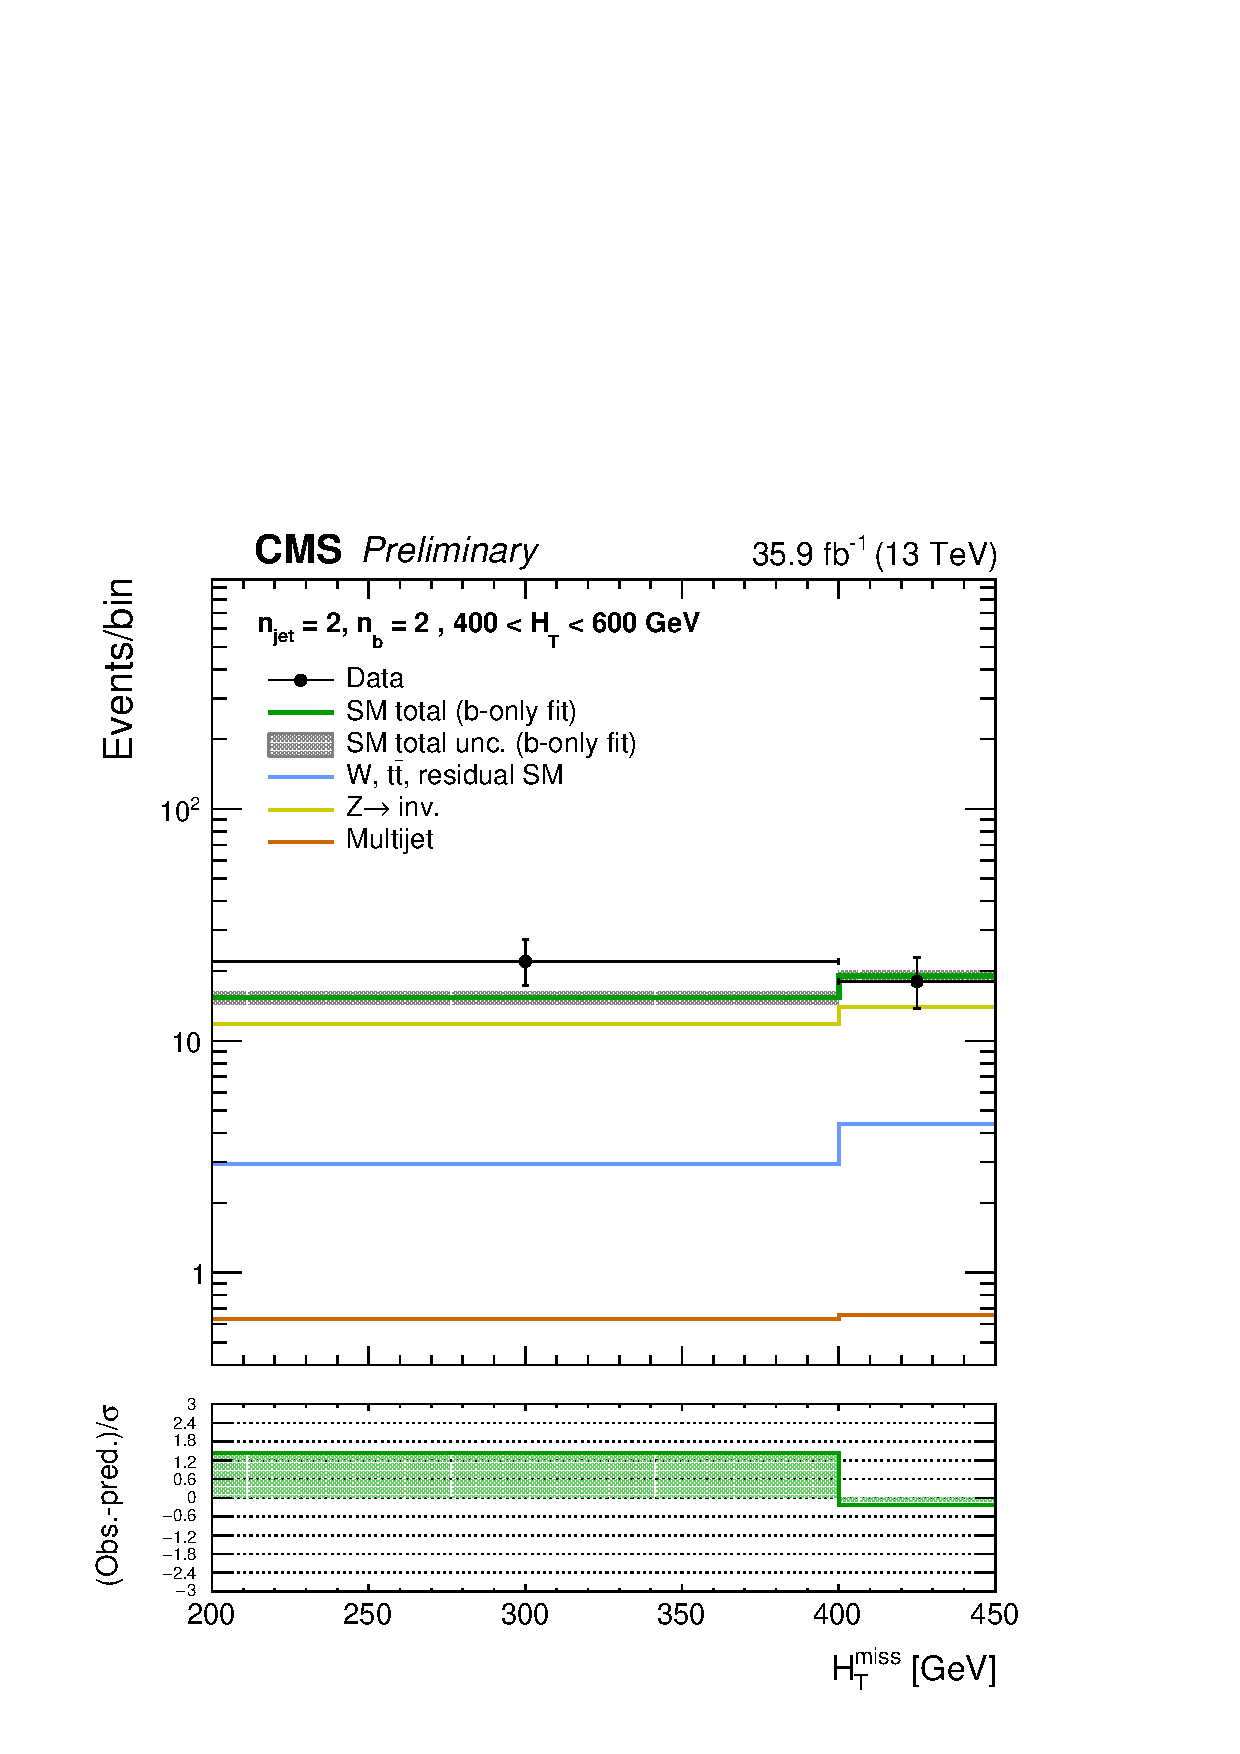
\includegraphics[width=0.49\textwidth]{figures/results/36invfb//crfit/shapes//mhtShape_eq2b_eq2j_400_600_fit_b.pdf}}
    \caption{Event yields observed in data (solid circles) and CR-fit SM expectations with their associated uncertainties (green histogram with shaded band) as a function of \HTmiss based on a sample of events that satisfy $\njet = 2$ and $\nb = 2$, as well as the requirements on \scalht indicated by each sub-figure caption. }
    \label{fig:mhtval_eq2j_eq2b}
  \end{center}
\end{figure}

\begin{figure}[h!]
  \begin{center}
    \subfigure[$400 < \scalht < 600\GeV$]{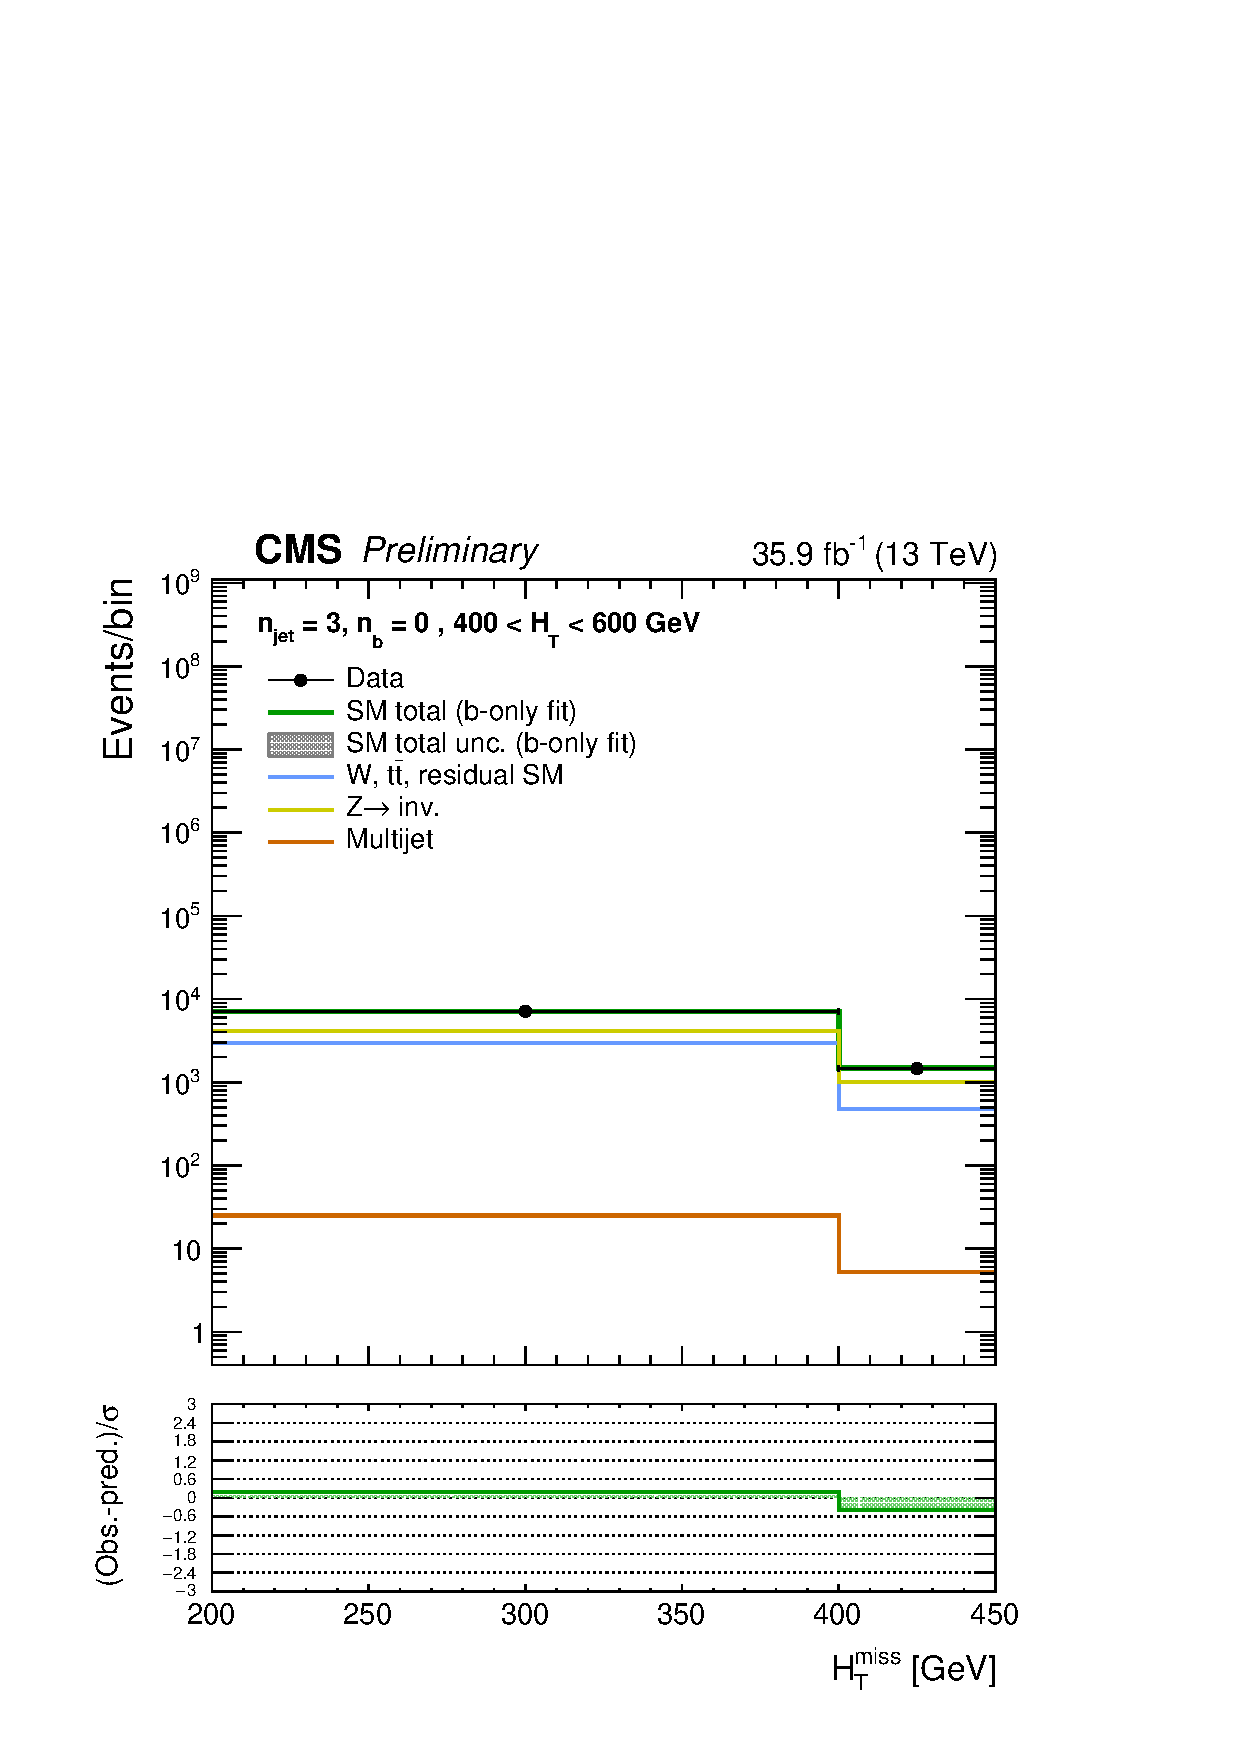
\includegraphics[width=0.49\textwidth]{figures/results/36invfb//crfit/shapes//mhtShape_eq0b_eq3j_400_600_fit_b.pdf}}
    \subfigure[$600 < \scalht < 900\GeV$]{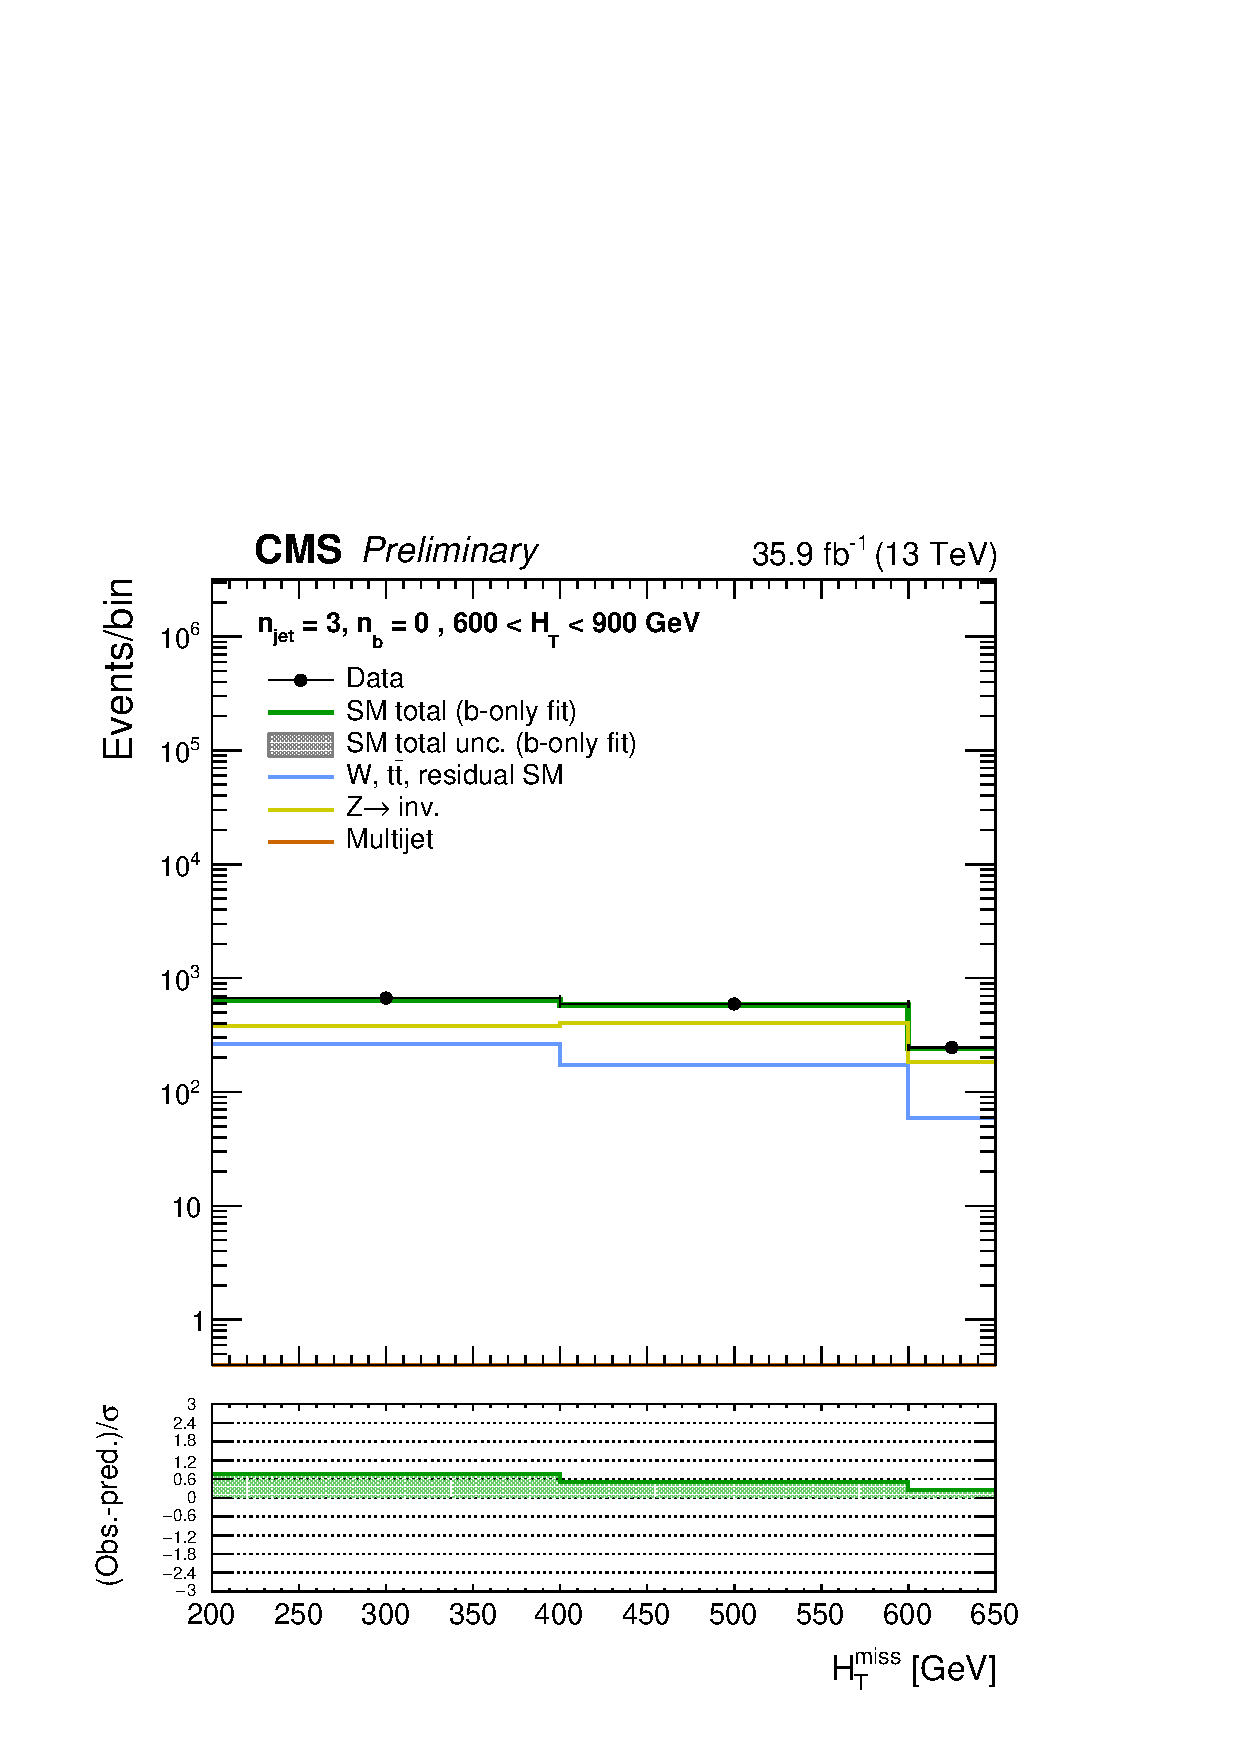
\includegraphics[width=0.49\textwidth]{figures/results/36invfb//crfit/shapes//mhtShape_eq0b_eq3j_600_900_fit_b.pdf}}\\
    \subfigure[$900 < \scalht < 1200\GeV$]{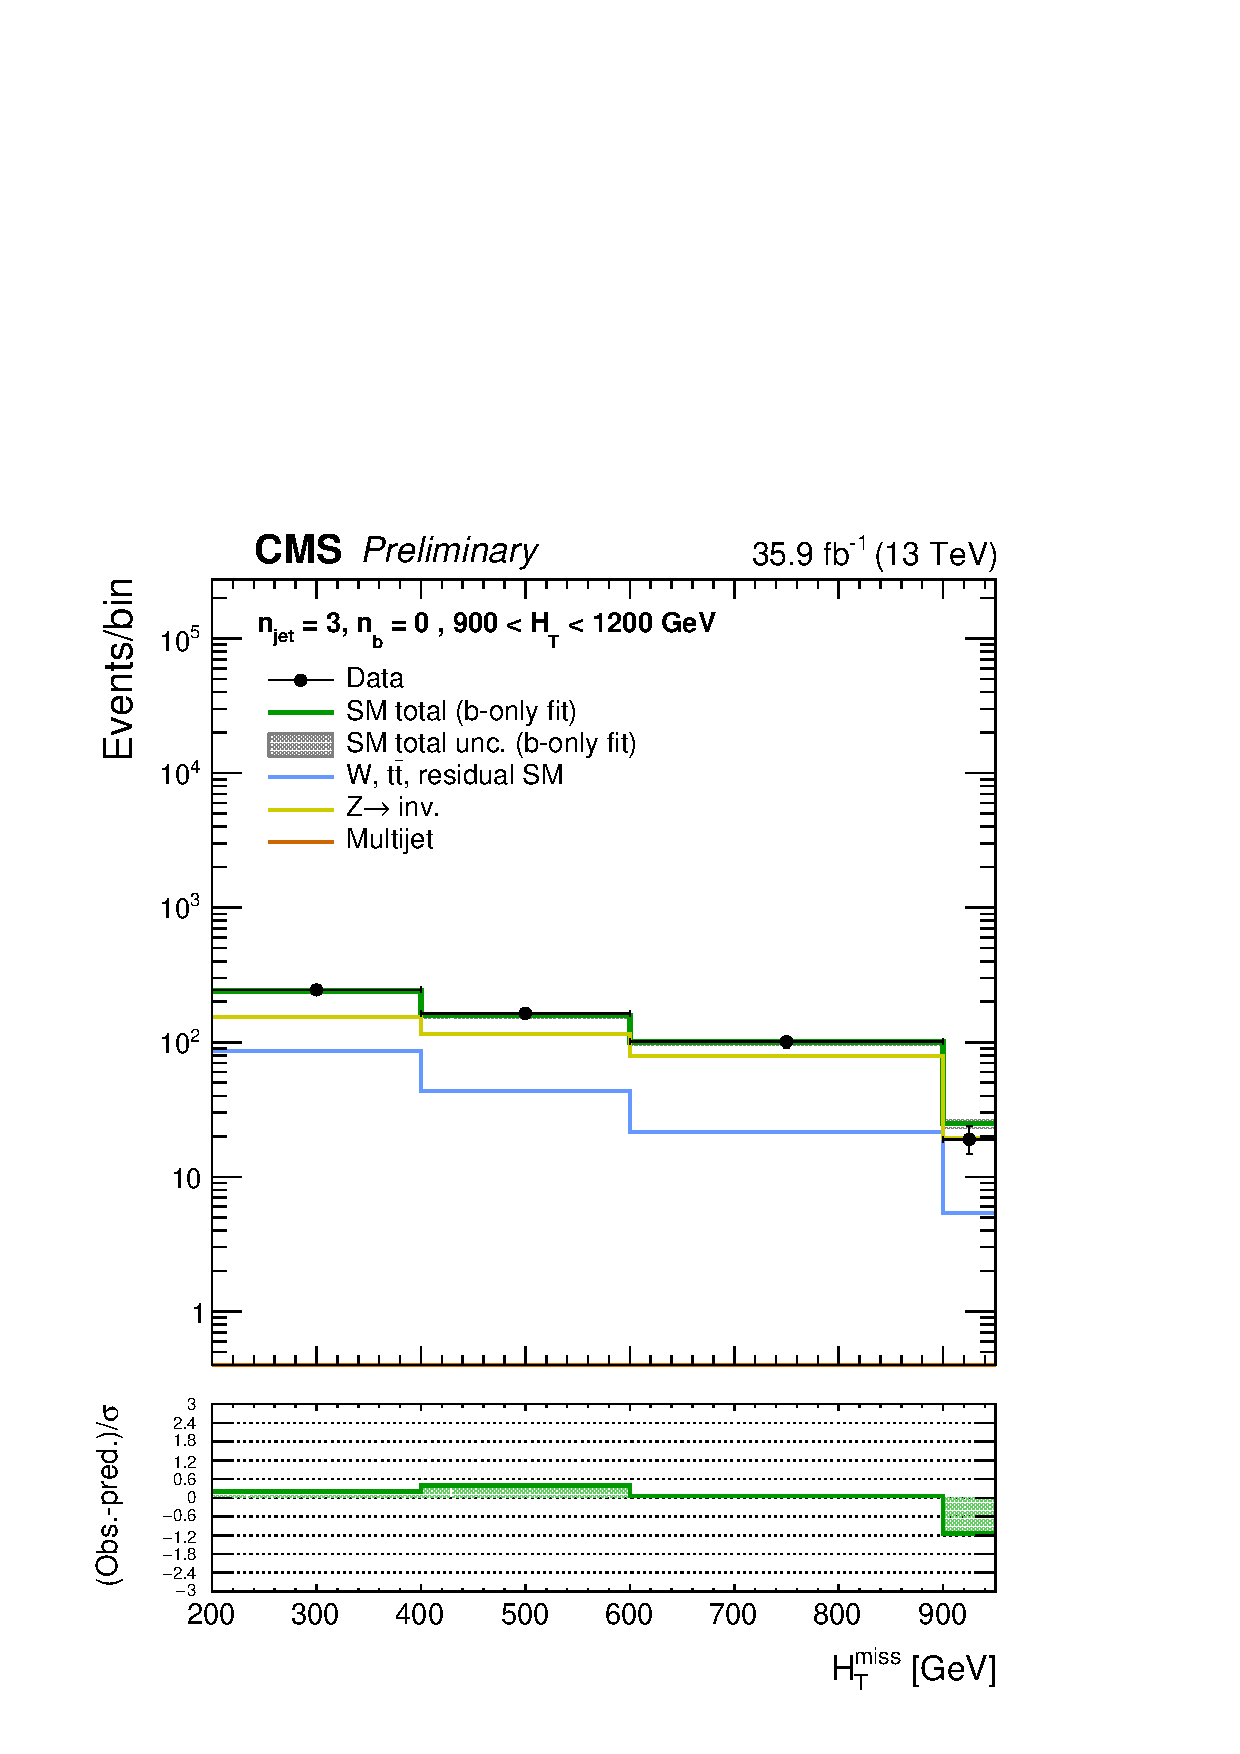
\includegraphics[width=0.49\textwidth]{figures/results/36invfb//crfit/shapes//mhtShape_eq0b_eq3j_900_1200_fit_b.pdf}}
    \subfigure[$\scalht > 1200\GeV$]{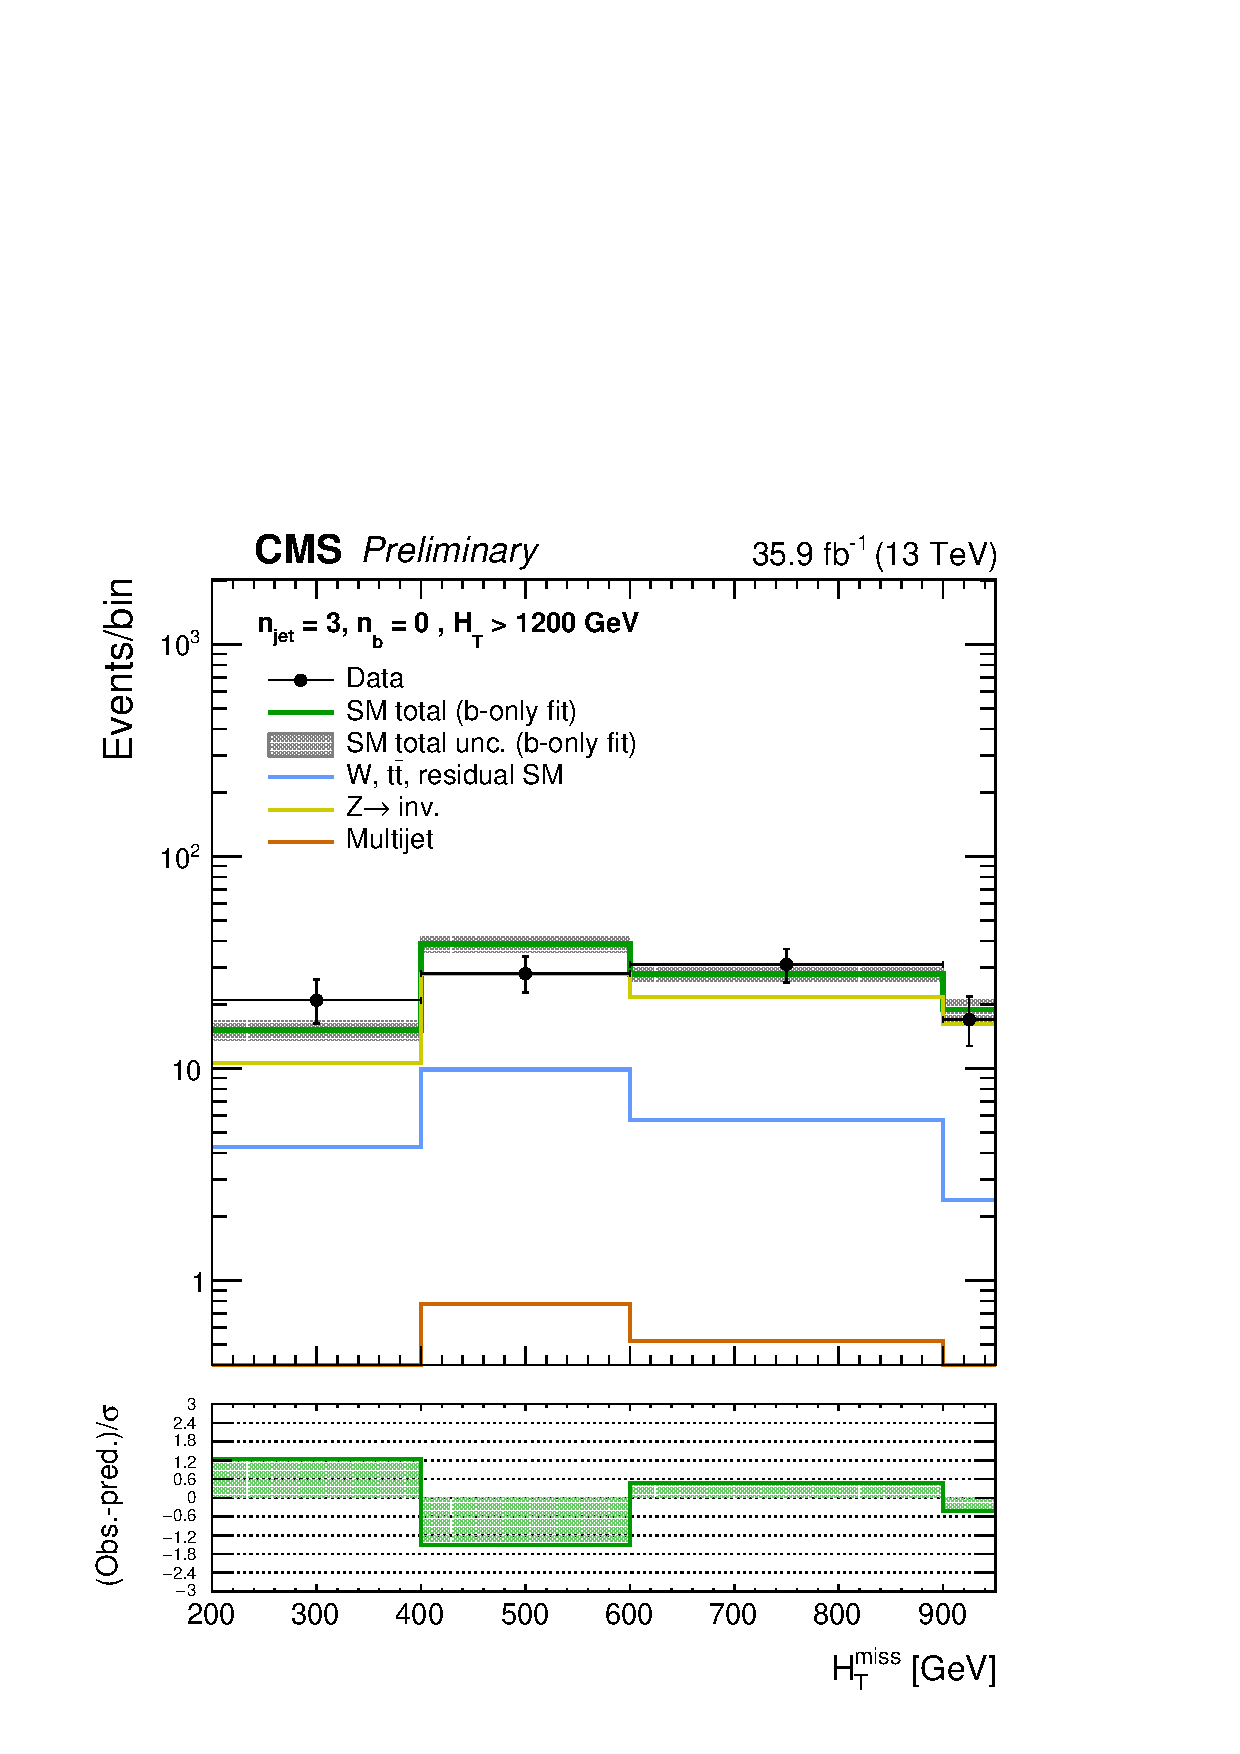
\includegraphics[width=0.49\textwidth]{figures/results/36invfb//crfit/shapes//mhtShape_eq0b_eq3j_1200_Inf_fit_b.pdf}}\\
    \caption{Event yields observed in data (solid circles) and CR-fit SM expectations with their associated uncertainties (green histogram with shaded band) as a function of \HTmiss based on a sample of events that satisfy $\njet = 3$ and $\nb = 0$, as well as the requirements on \scalht indicated by each sub-figure caption. }
    \label{fig:mhtval_eq3j_eq0b}
  \end{center}
\end{figure}

\begin{figure}[h!]
  \begin{center}
    \subfigure[$400 < \scalht < 600\GeV$]{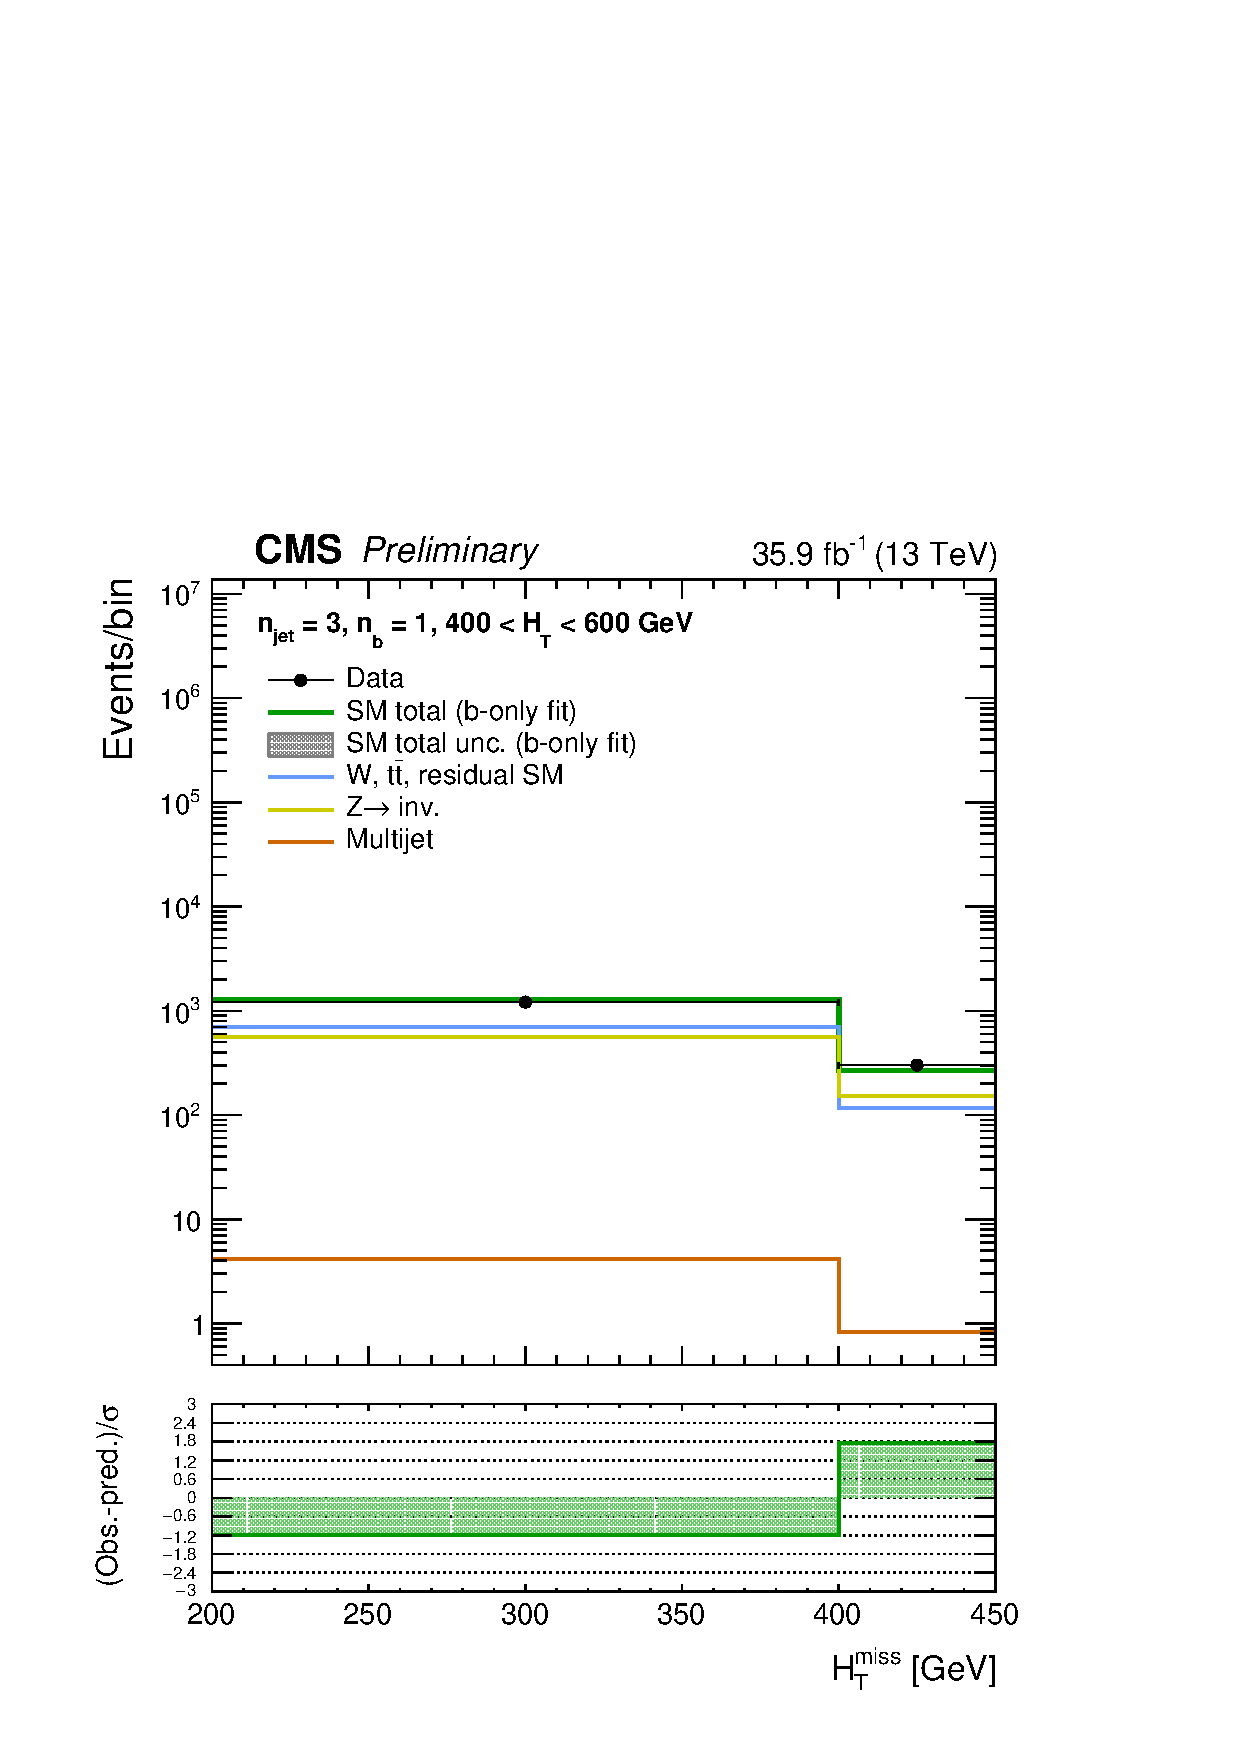
\includegraphics[width=0.49\textwidth]{figures/results/36invfb//crfit/shapes//mhtShape_eq1b_eq3j_400_600_fit_b.pdf}}
    \subfigure[$600 < \scalht < 900\GeV$]{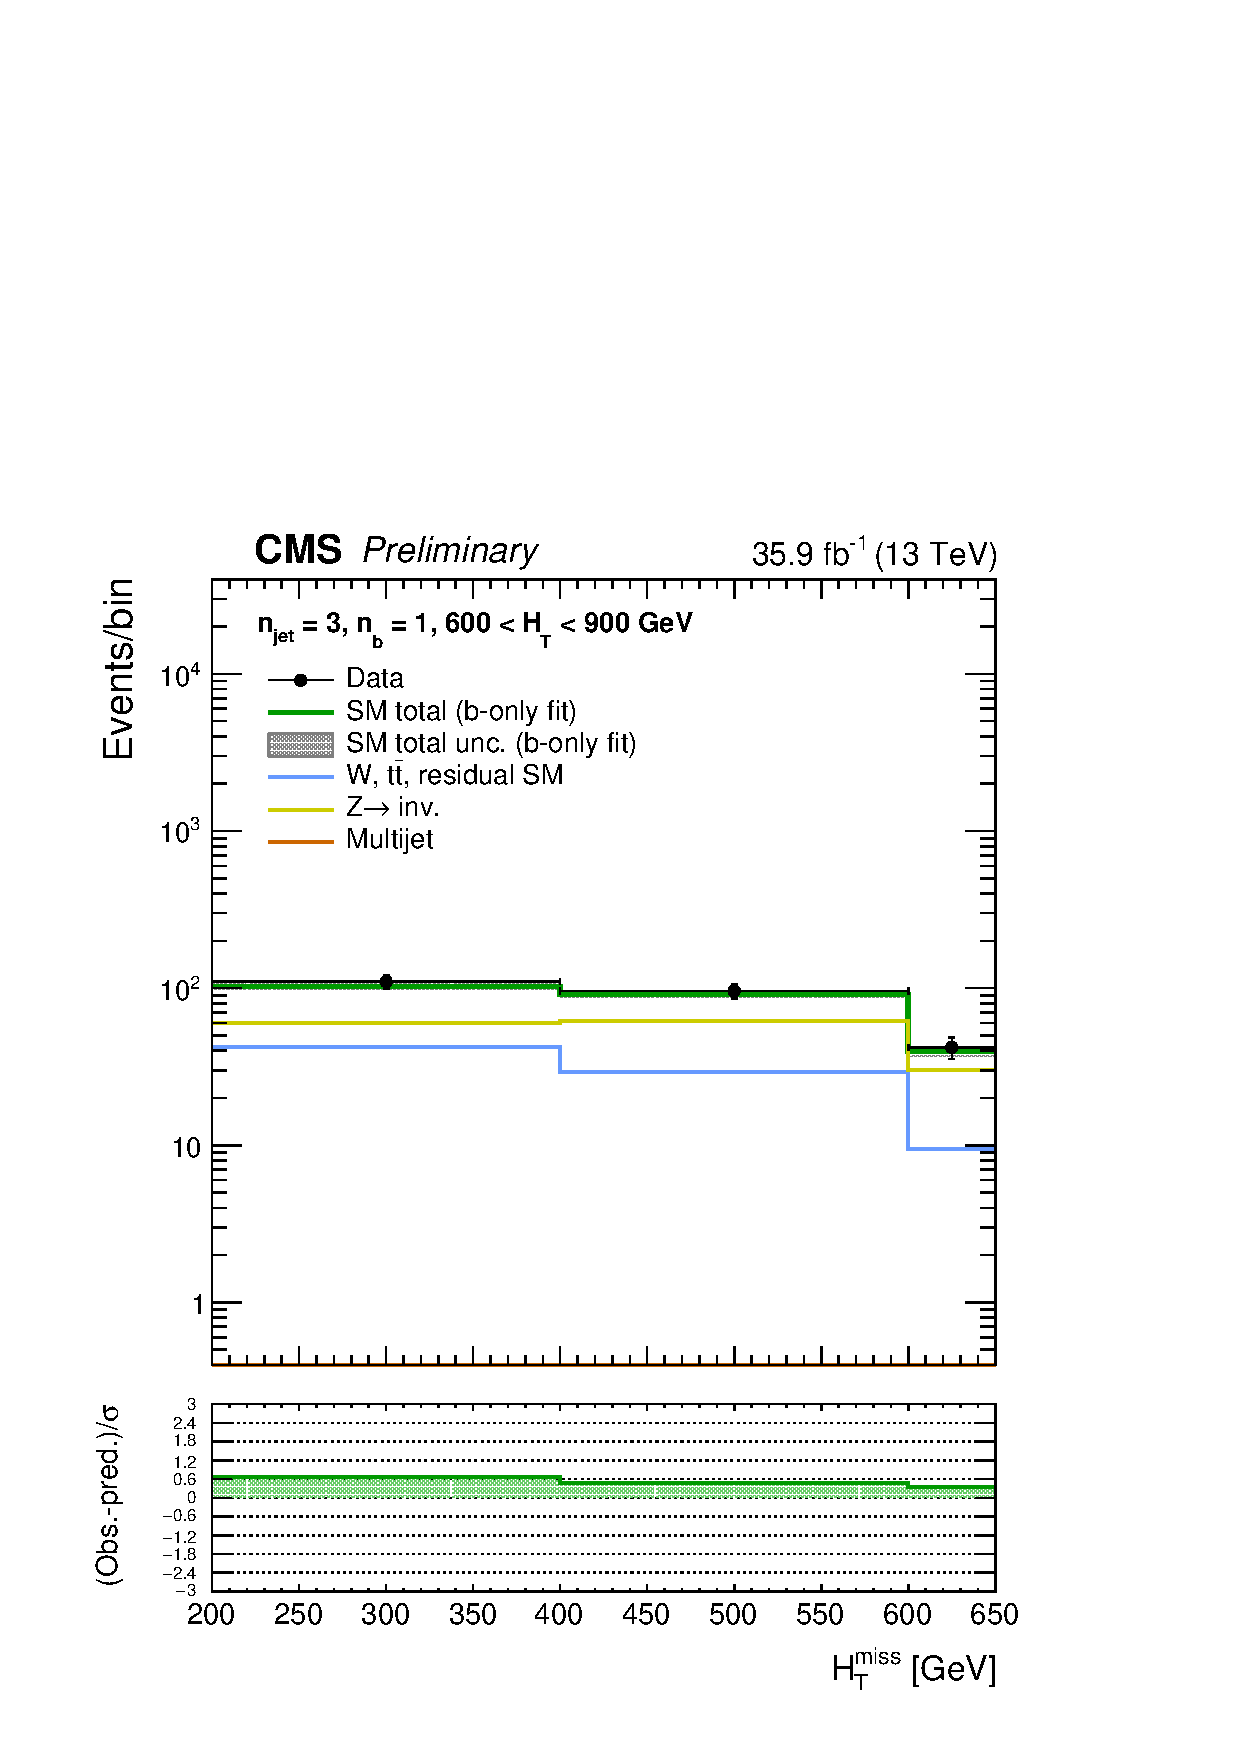
\includegraphics[width=0.49\textwidth]{figures/results/36invfb//crfit/shapes//mhtShape_eq1b_eq3j_600_900_fit_b.pdf}}\\
    \subfigure[$900 < \scalht < 1200\GeV$]{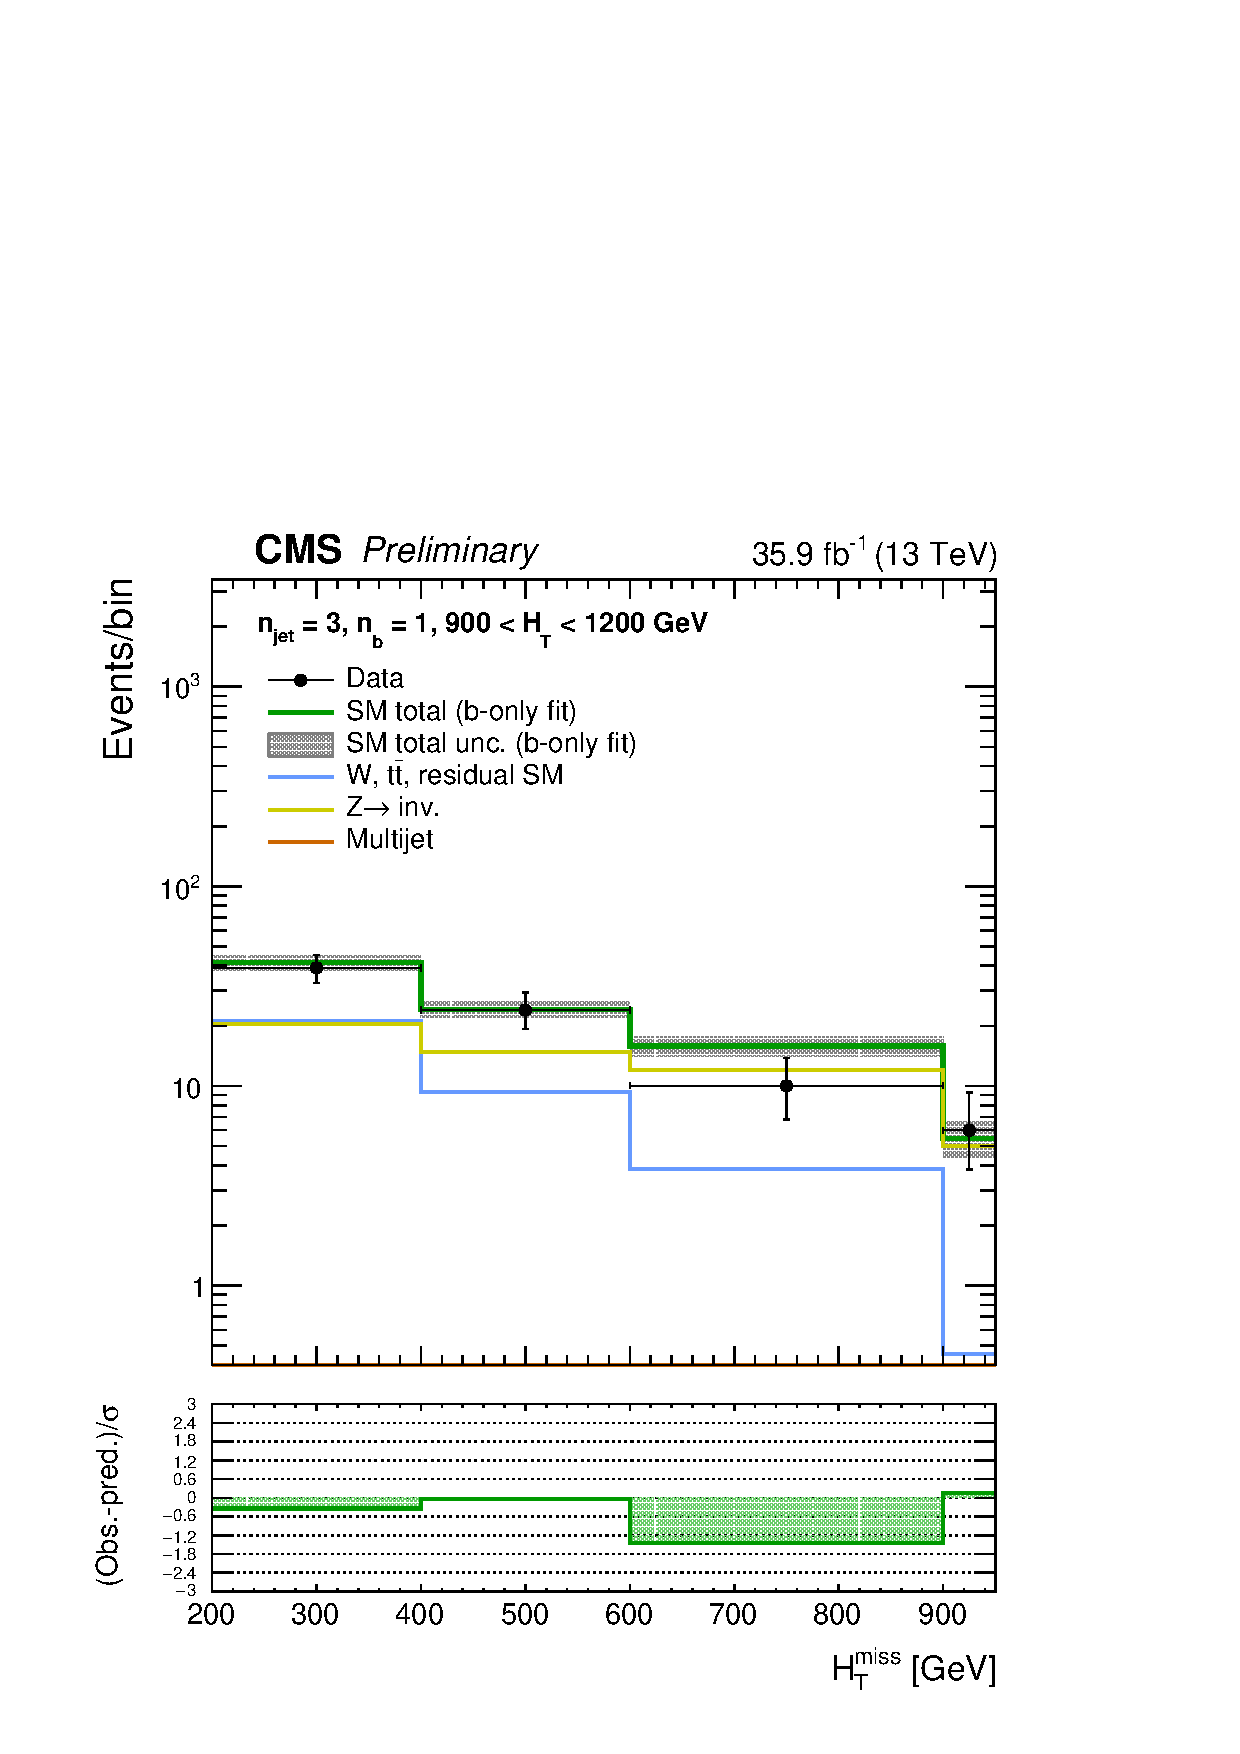
\includegraphics[width=0.49\textwidth]{figures/results/36invfb//crfit/shapes//mhtShape_eq1b_eq3j_900_1200_fit_b.pdf}}
    \subfigure[$\scalht > 1200\GeV$]{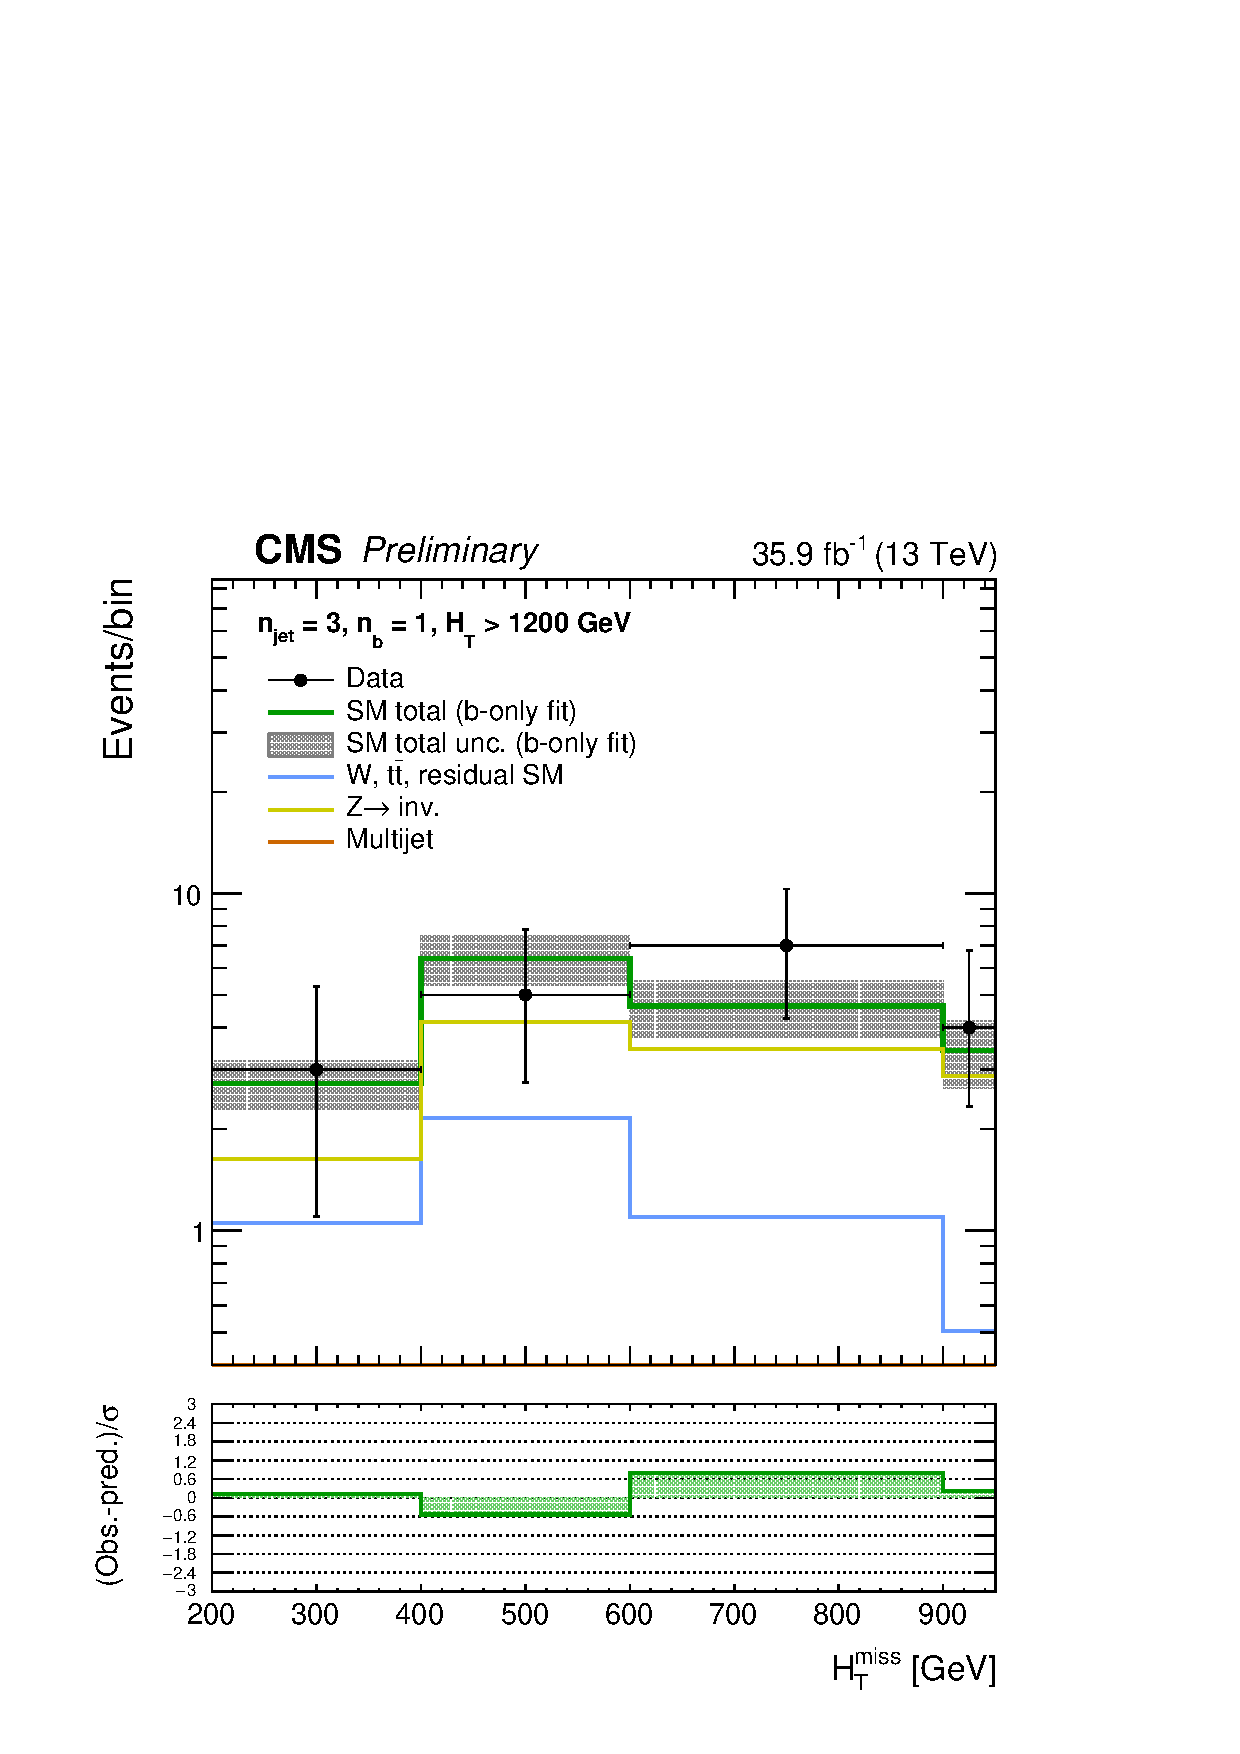
\includegraphics[width=0.49\textwidth]{figures/results/36invfb//crfit/shapes//mhtShape_eq1b_eq3j_1200_Inf_fit_b.pdf}}\\
    \caption{Event yields observed in data (solid circles) and CR-fit SM expectations with their associated uncertainties (green histogram with shaded band) as a function of \HTmiss based on a sample of events that satisfy $\njet = 3$ and $\nb = 1$, as well as the requirements on \scalht indicated by each sub-figure caption. }
    \label{fig:mhtval_eq3j_eq1b}
  \end{center}
\end{figure}

\begin{figure}[h!]
  \begin{center}
    \subfigure[$400 < \scalht < 600\GeV$]{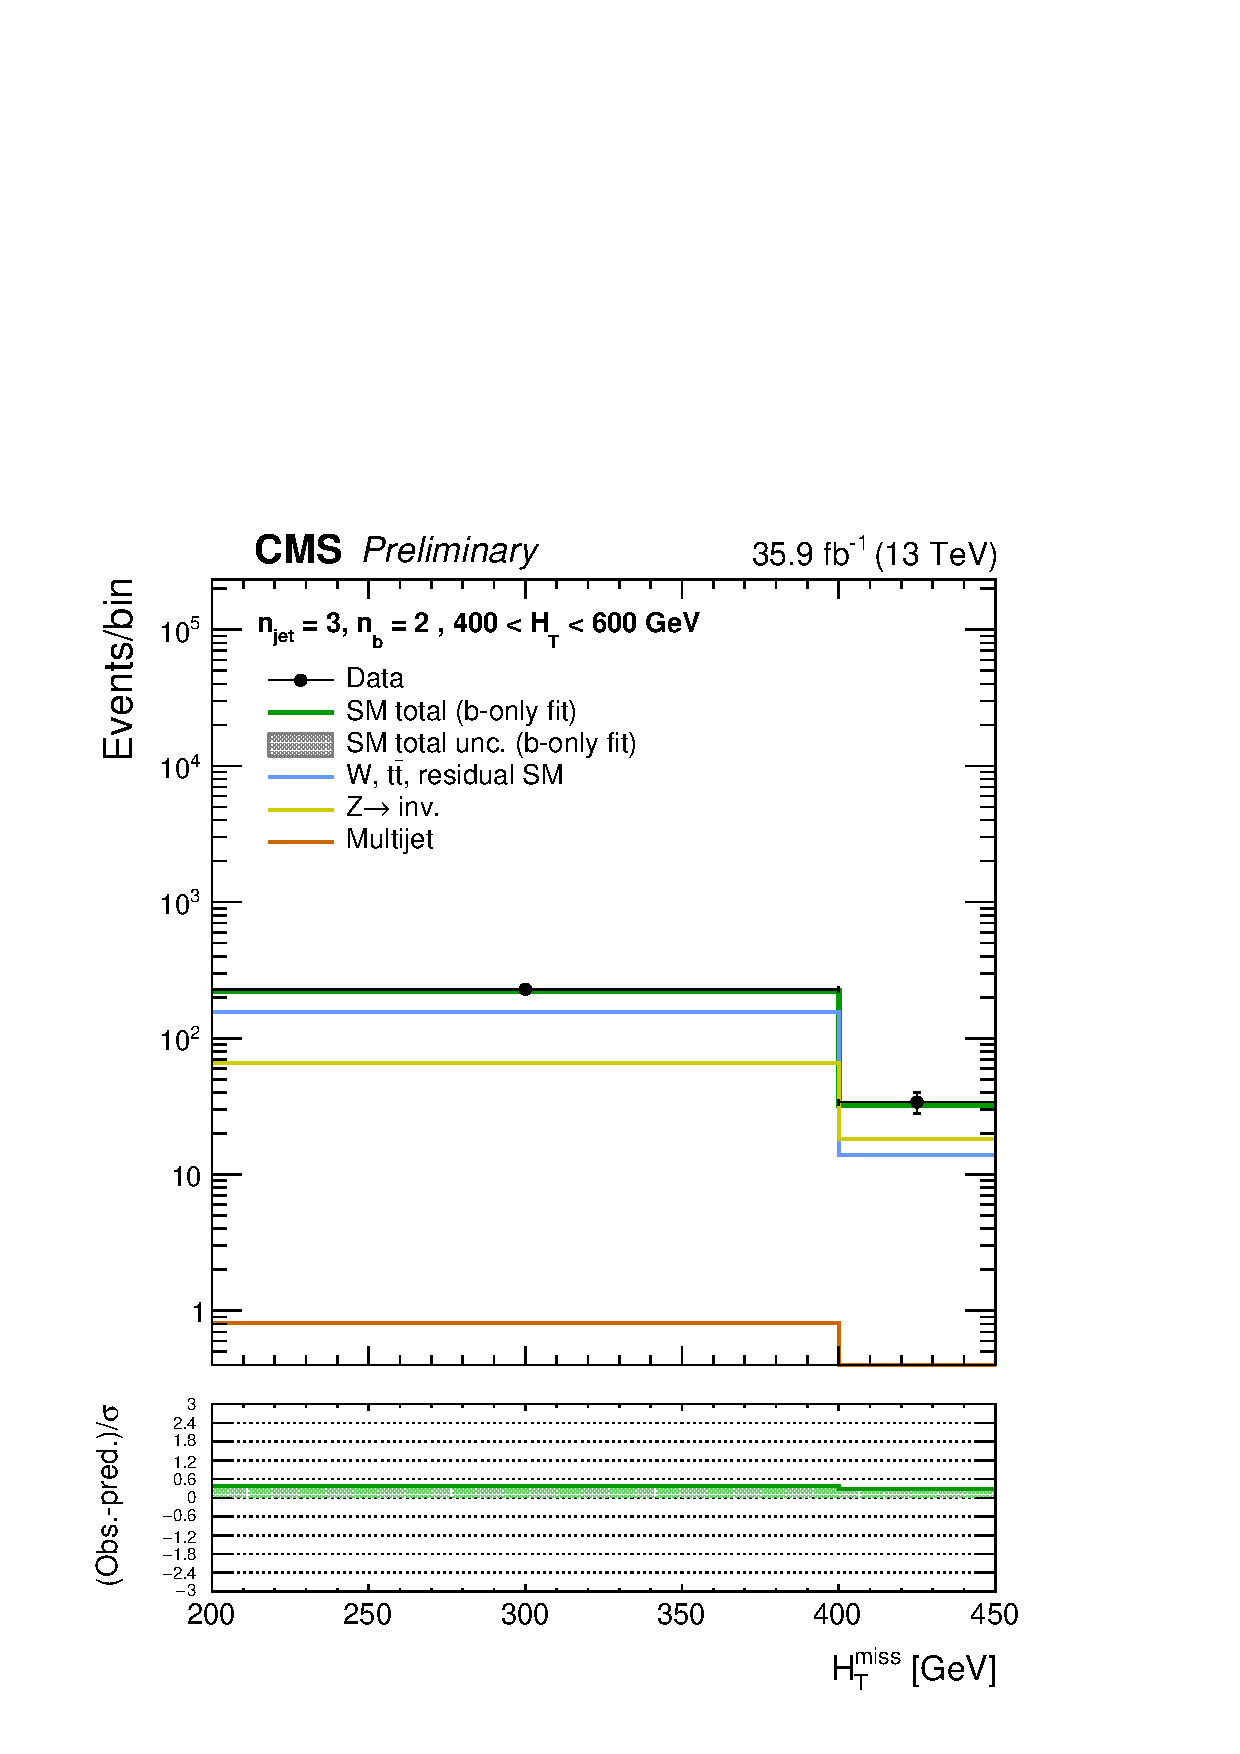
\includegraphics[width=0.49\textwidth]{figures/results/36invfb//crfit/shapes//mhtShape_eq2b_eq3j_400_600_fit_b.pdf}}
    \subfigure[$600 < \scalht < 900\GeV$]{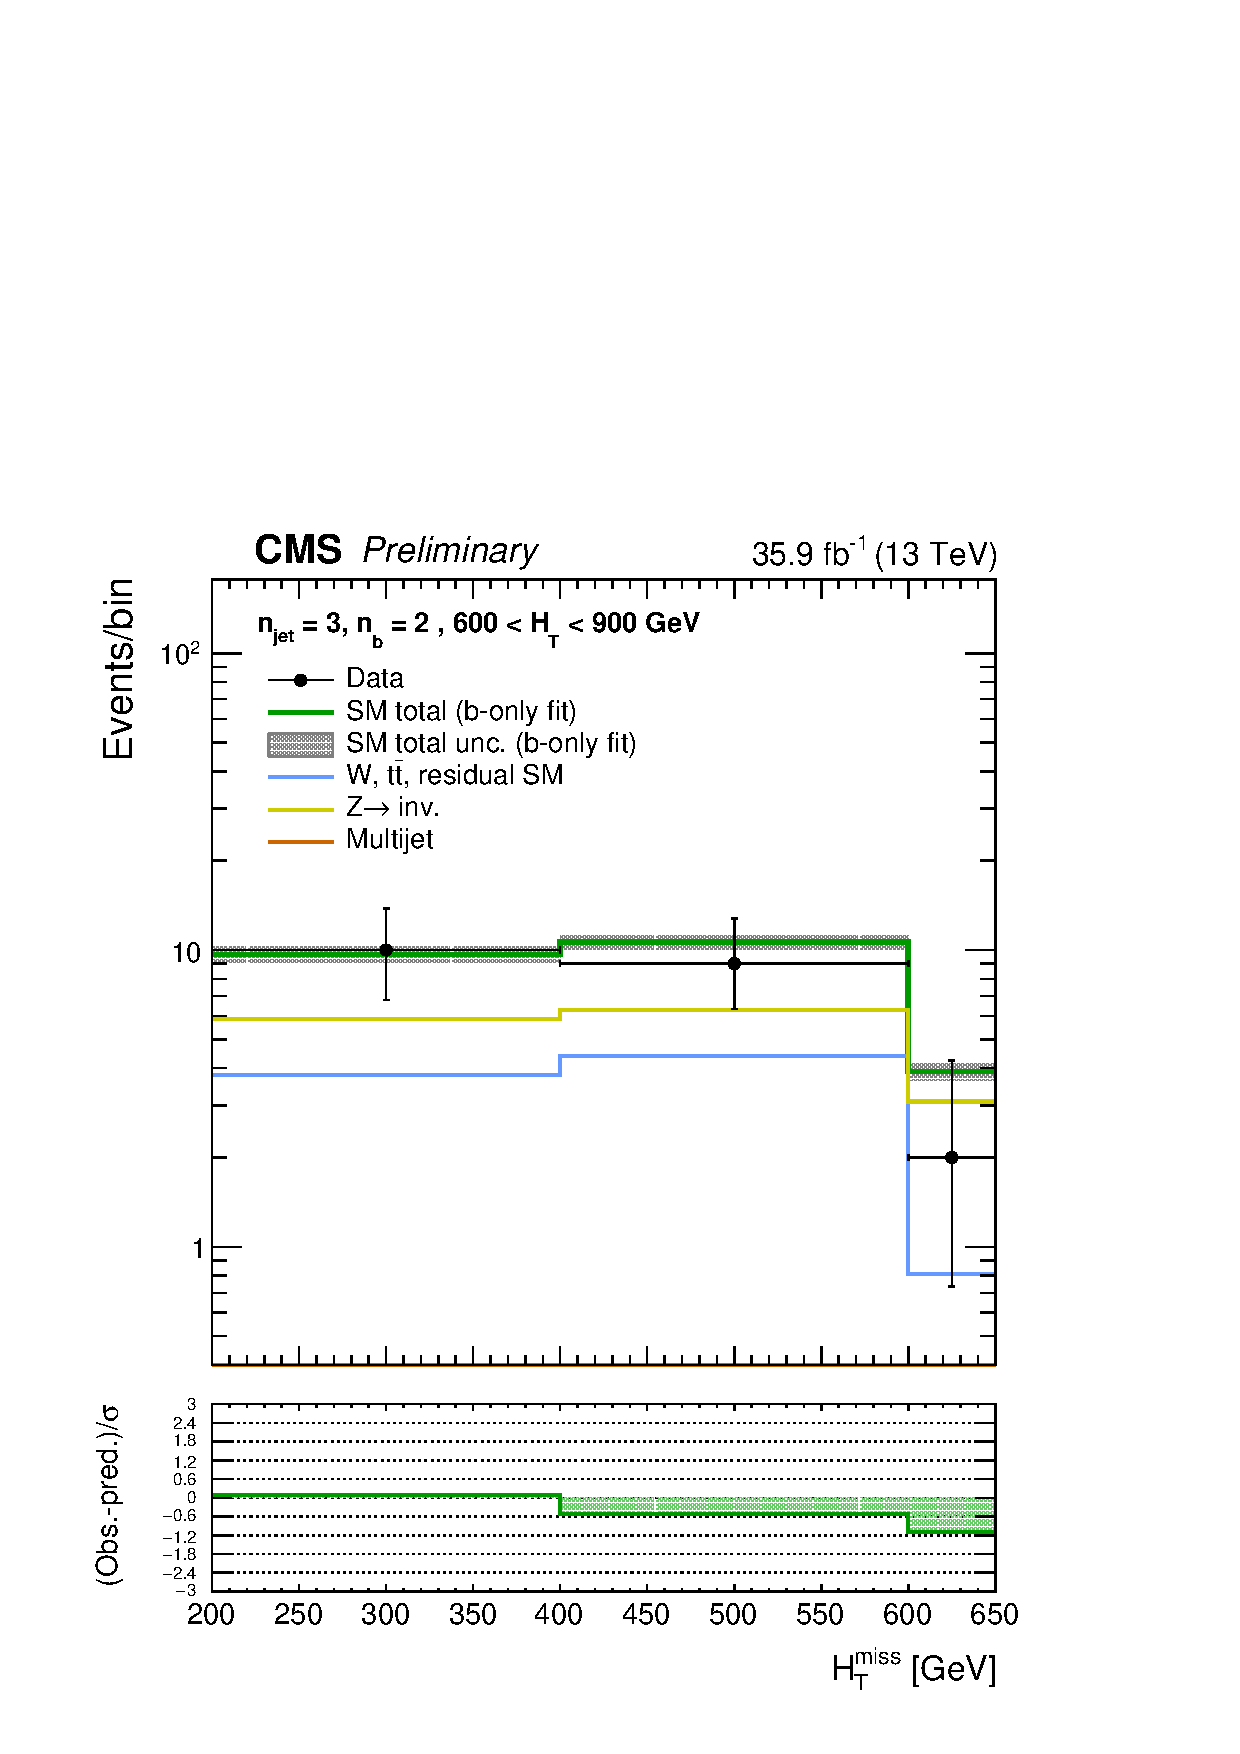
\includegraphics[width=0.49\textwidth]{figures/results/36invfb//crfit/shapes//mhtShape_eq2b_eq3j_600_900_fit_b.pdf}}\\
    \subfigure[$900 < \scalht < 1200\GeV$]{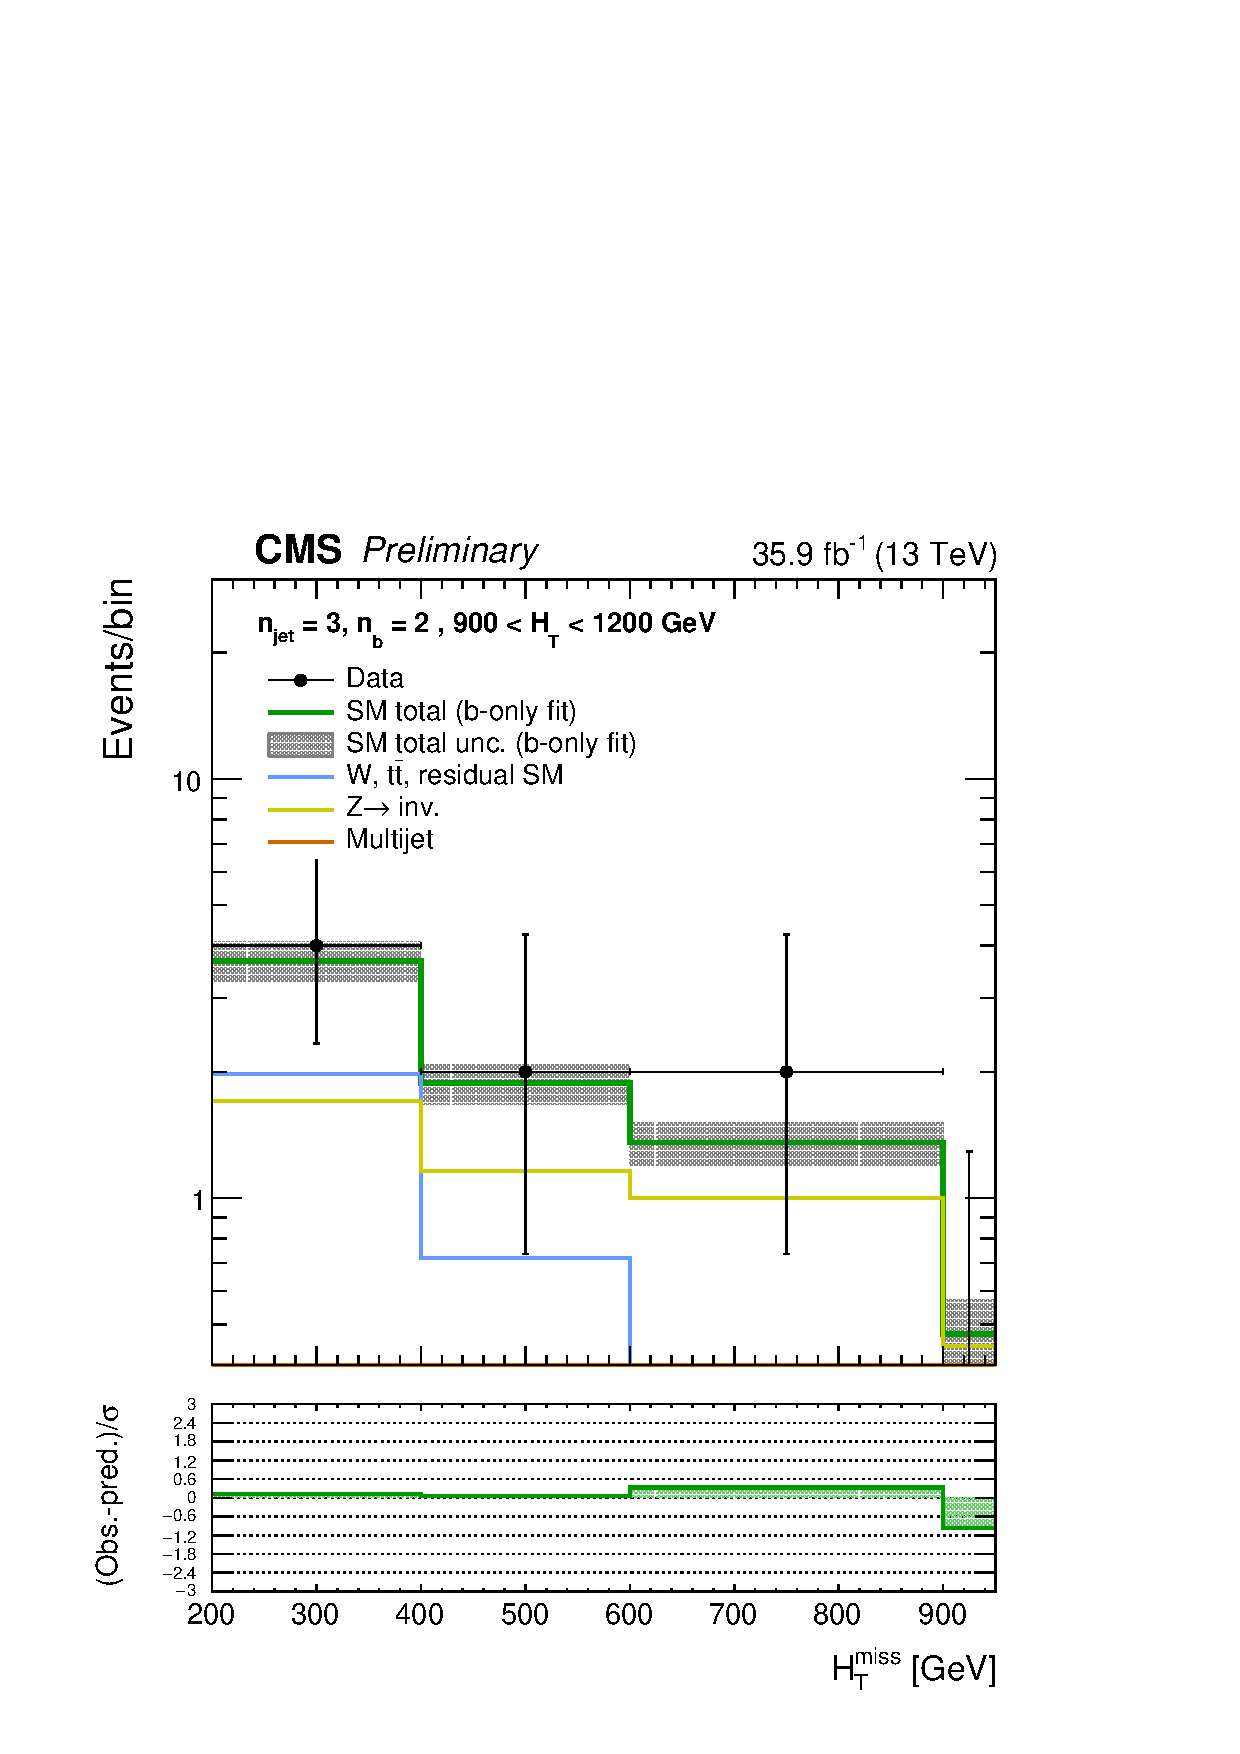
\includegraphics[width=0.49\textwidth]{figures/results/36invfb//crfit/shapes//mhtShape_eq2b_eq3j_900_1200_fit_b.pdf}}
    \subfigure[$\scalht > 1200\GeV$]{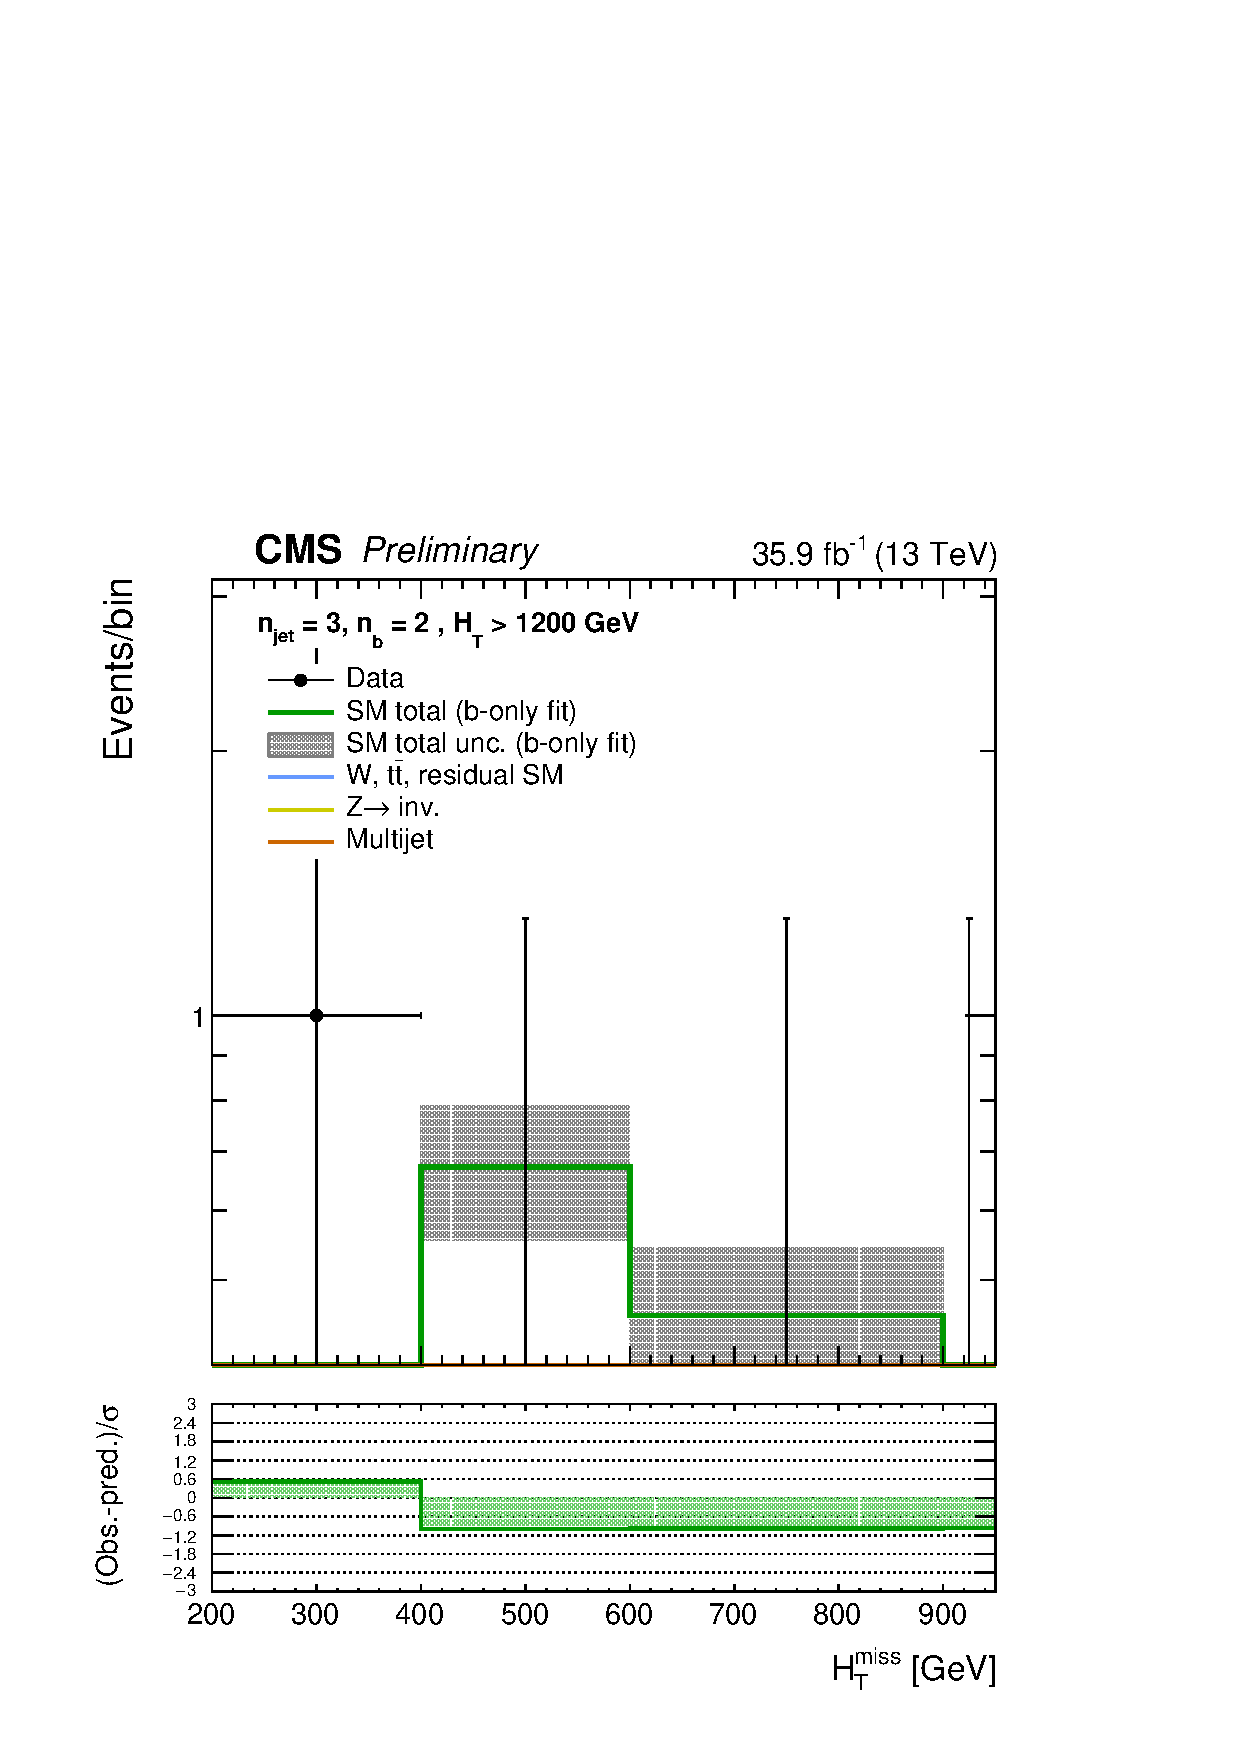
\includegraphics[width=0.49\textwidth]{figures/results/36invfb//crfit/shapes//mhtShape_eq2b_eq3j_1200_Inf_fit_b.pdf}}\\
    \caption{Event yields observed in data (solid circles) and CR-fit SM expectations with their associated uncertainties (green histogram with shaded band) as a function of \HTmiss based on a sample of events that satisfy $\njet = 3$ and $\nb = 2$, as well as the requirements on \scalht indicated by each sub-figure caption. }
    \label{fig:mhtval_eq3j_eq2b}
  \end{center}
\end{figure}

\begin{figure}[h!]
  \begin{center}
    \subfigure[$400 < \scalht < 600\GeV$]{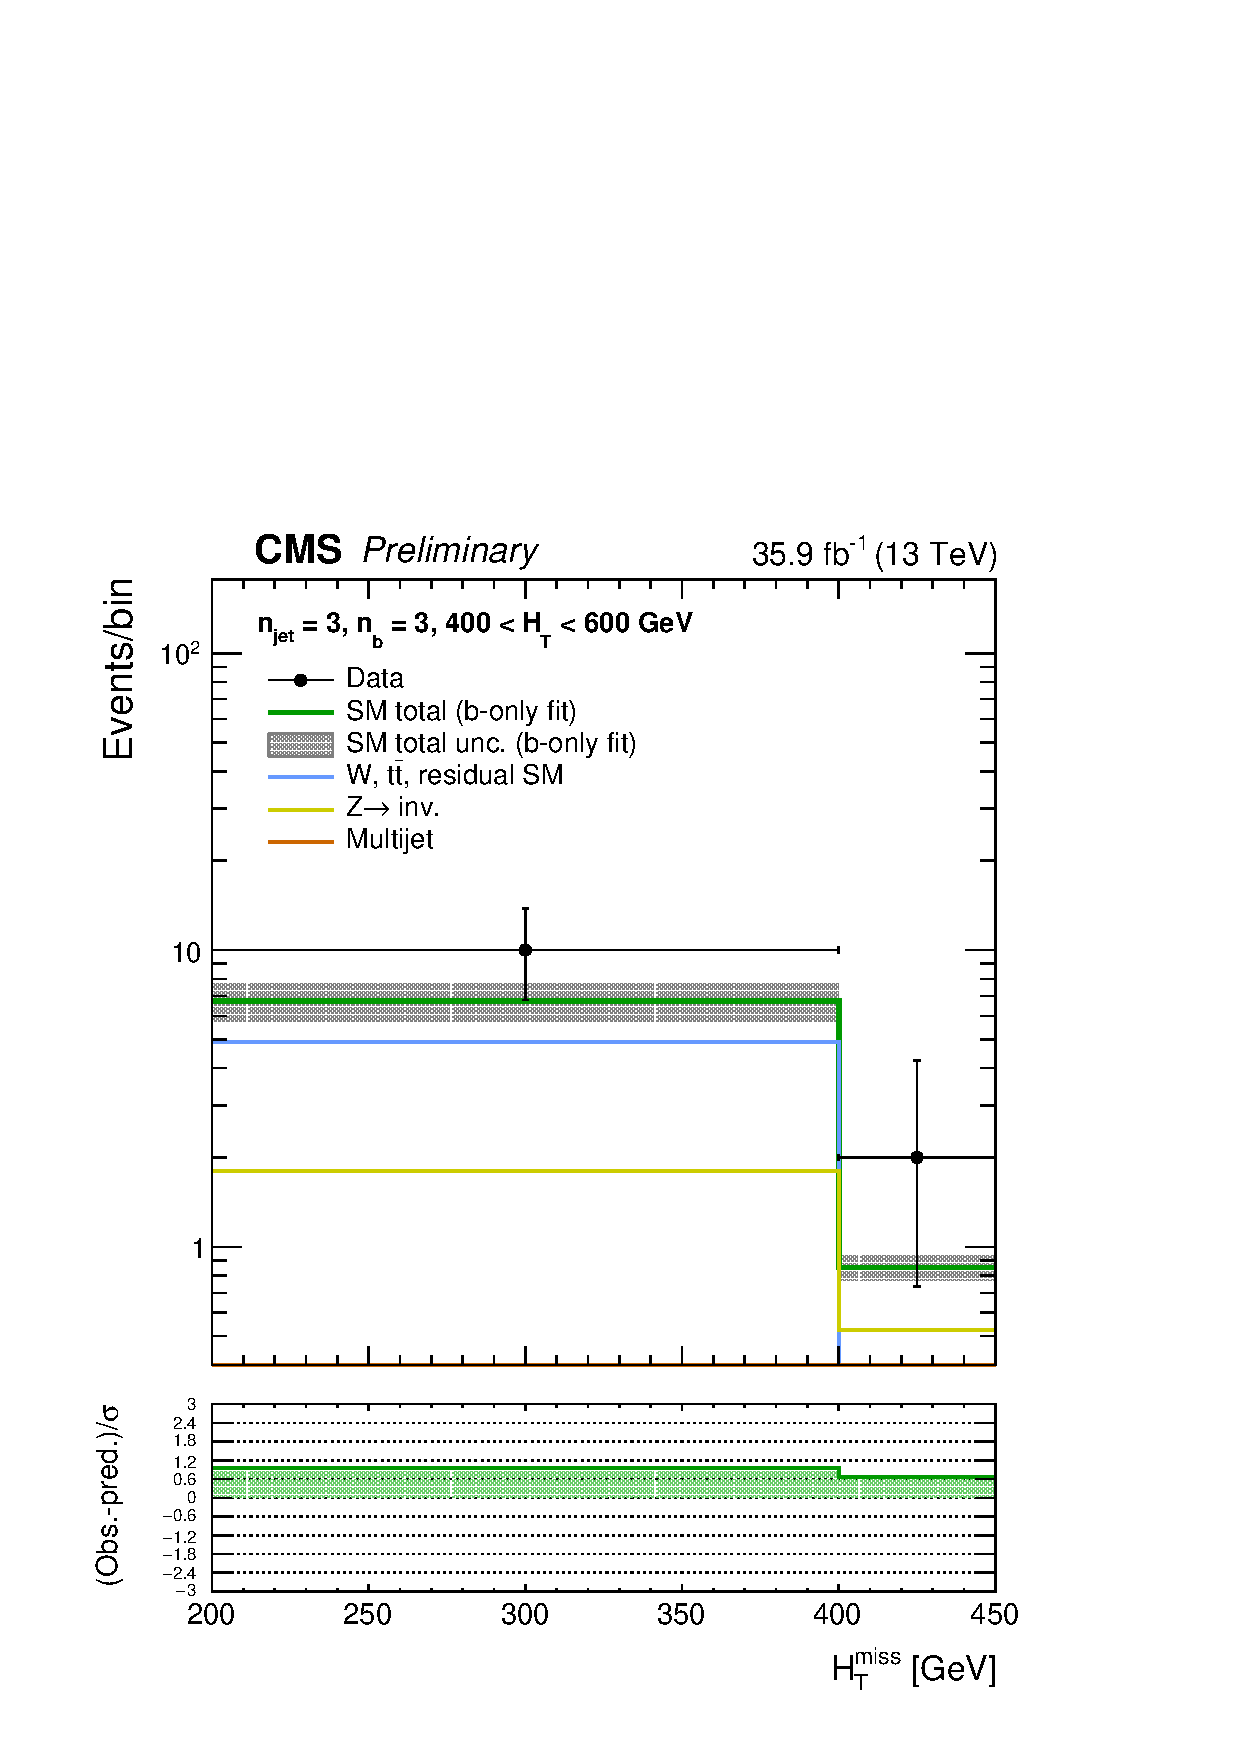
\includegraphics[width=0.49\textwidth]{figures/results/36invfb//crfit/shapes//mhtShape_eq3b_eq3j_400_600_fit_b.pdf}}
    \caption{Event yields observed in data (solid circles) and CR-fit SM expectations with their associated uncertainties (green histogram with shaded band) as a function of \HTmiss based on a sample of events that satisfy $\njet = 3$ and $\nb = 3$, as well as the requirements on \scalht indicated by each sub-figure caption. }
    \label{fig:mhtval_eq3j_eq3b}
  \end{center}
\end{figure}

\begin{figure}[h!]
  \begin{center}
    \subfigure[$400 < \scalht < 600\GeV$]{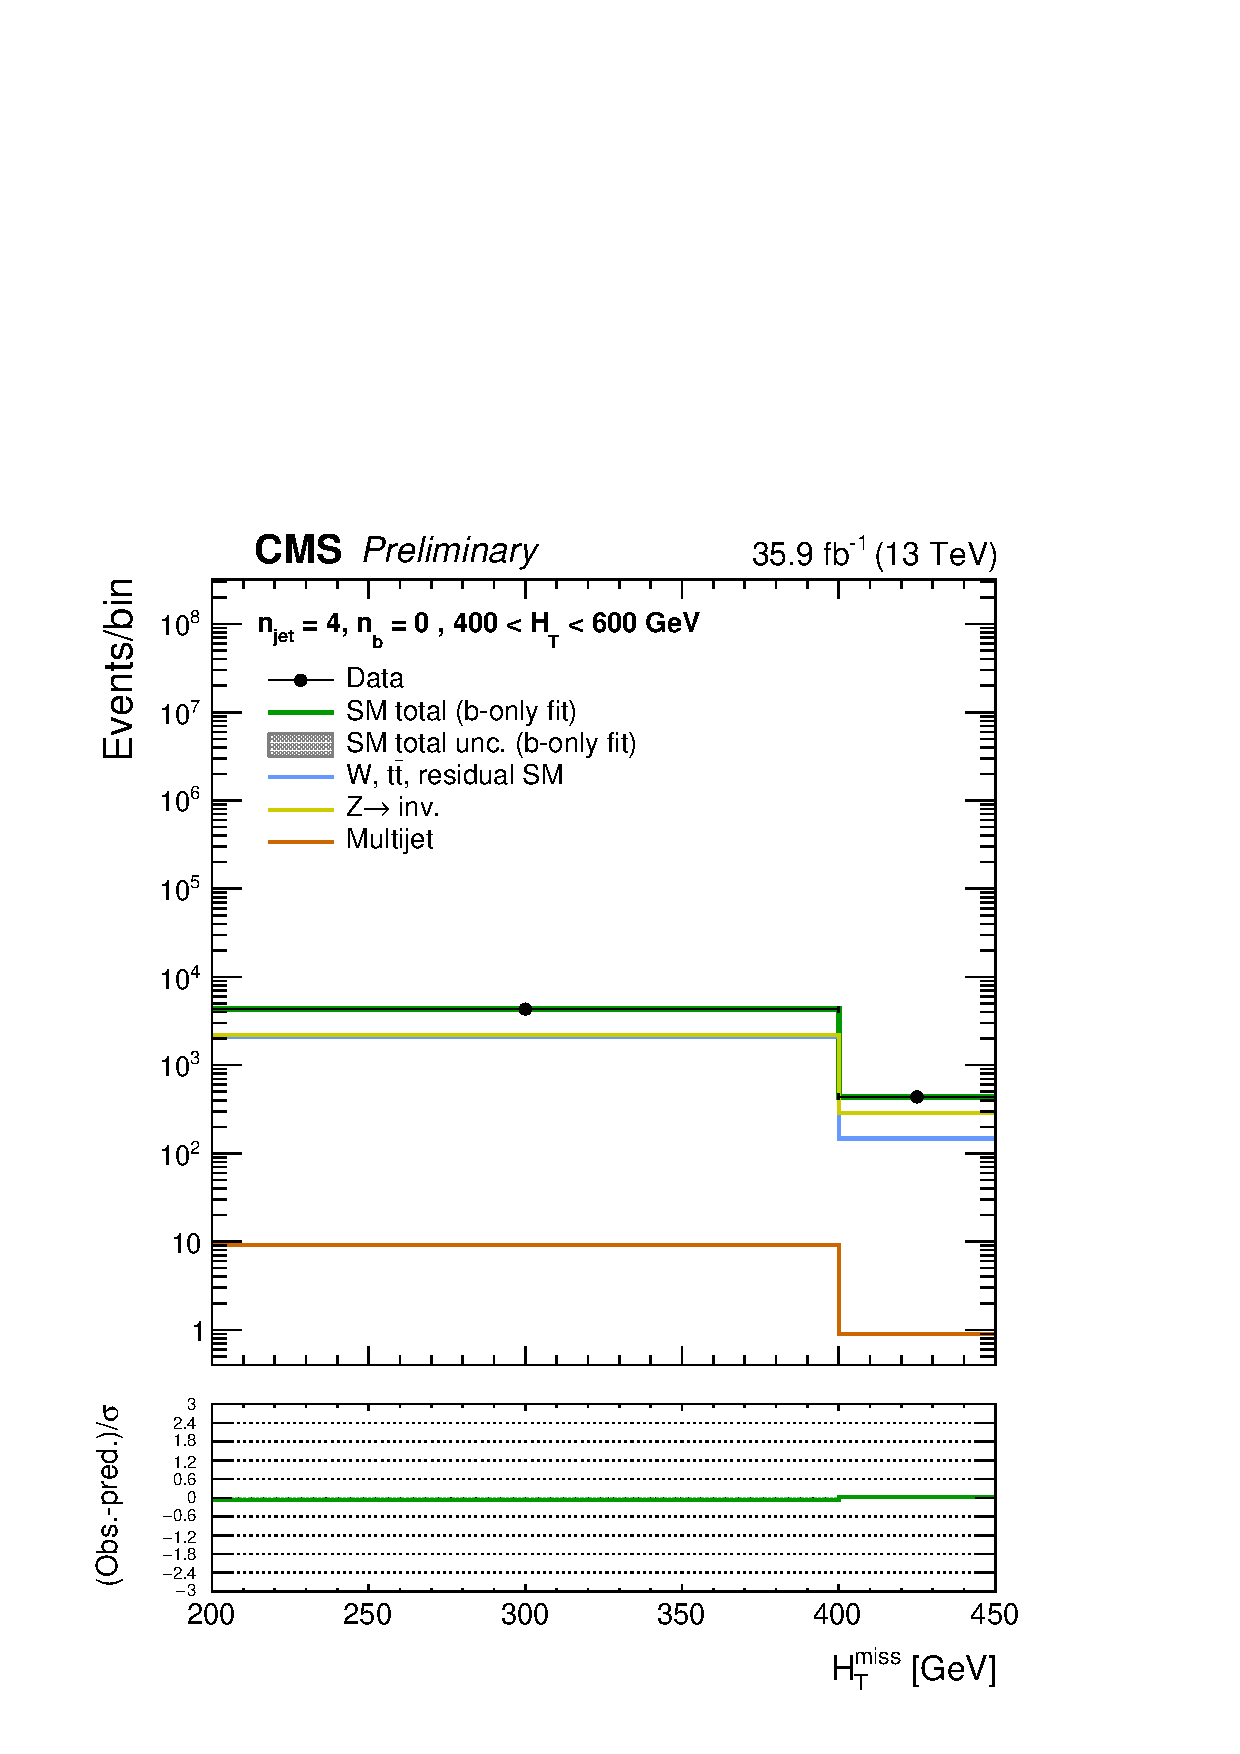
\includegraphics[width=0.49\textwidth]{figures/results/36invfb//crfit/shapes//mhtShape_eq0b_eq4j_400_600_fit_b.pdf}}
    \subfigure[$600 < \scalht < 900\GeV$]{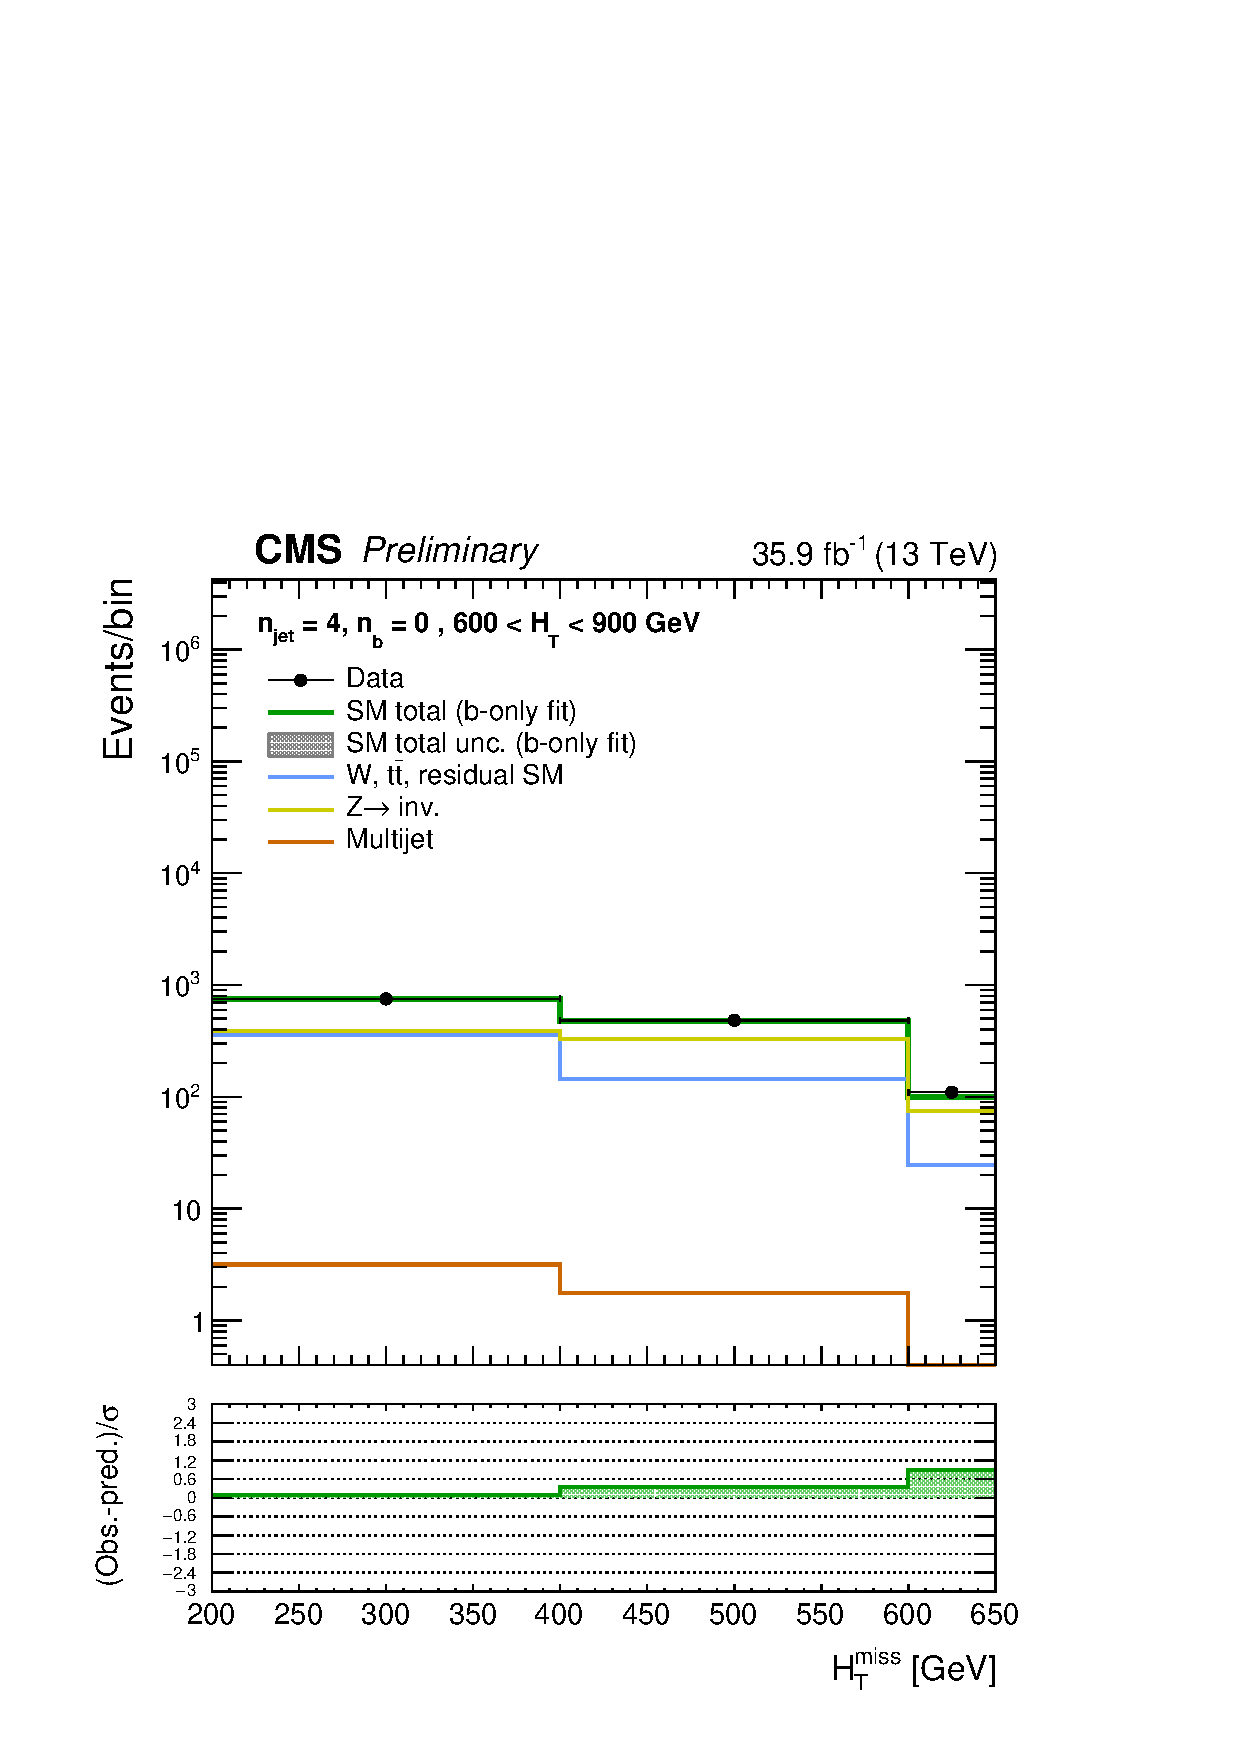
\includegraphics[width=0.49\textwidth]{figures/results/36invfb//crfit/shapes//mhtShape_eq0b_eq4j_600_900_fit_b.pdf}}\\
    \subfigure[$900 < \scalht < 1200\GeV$]{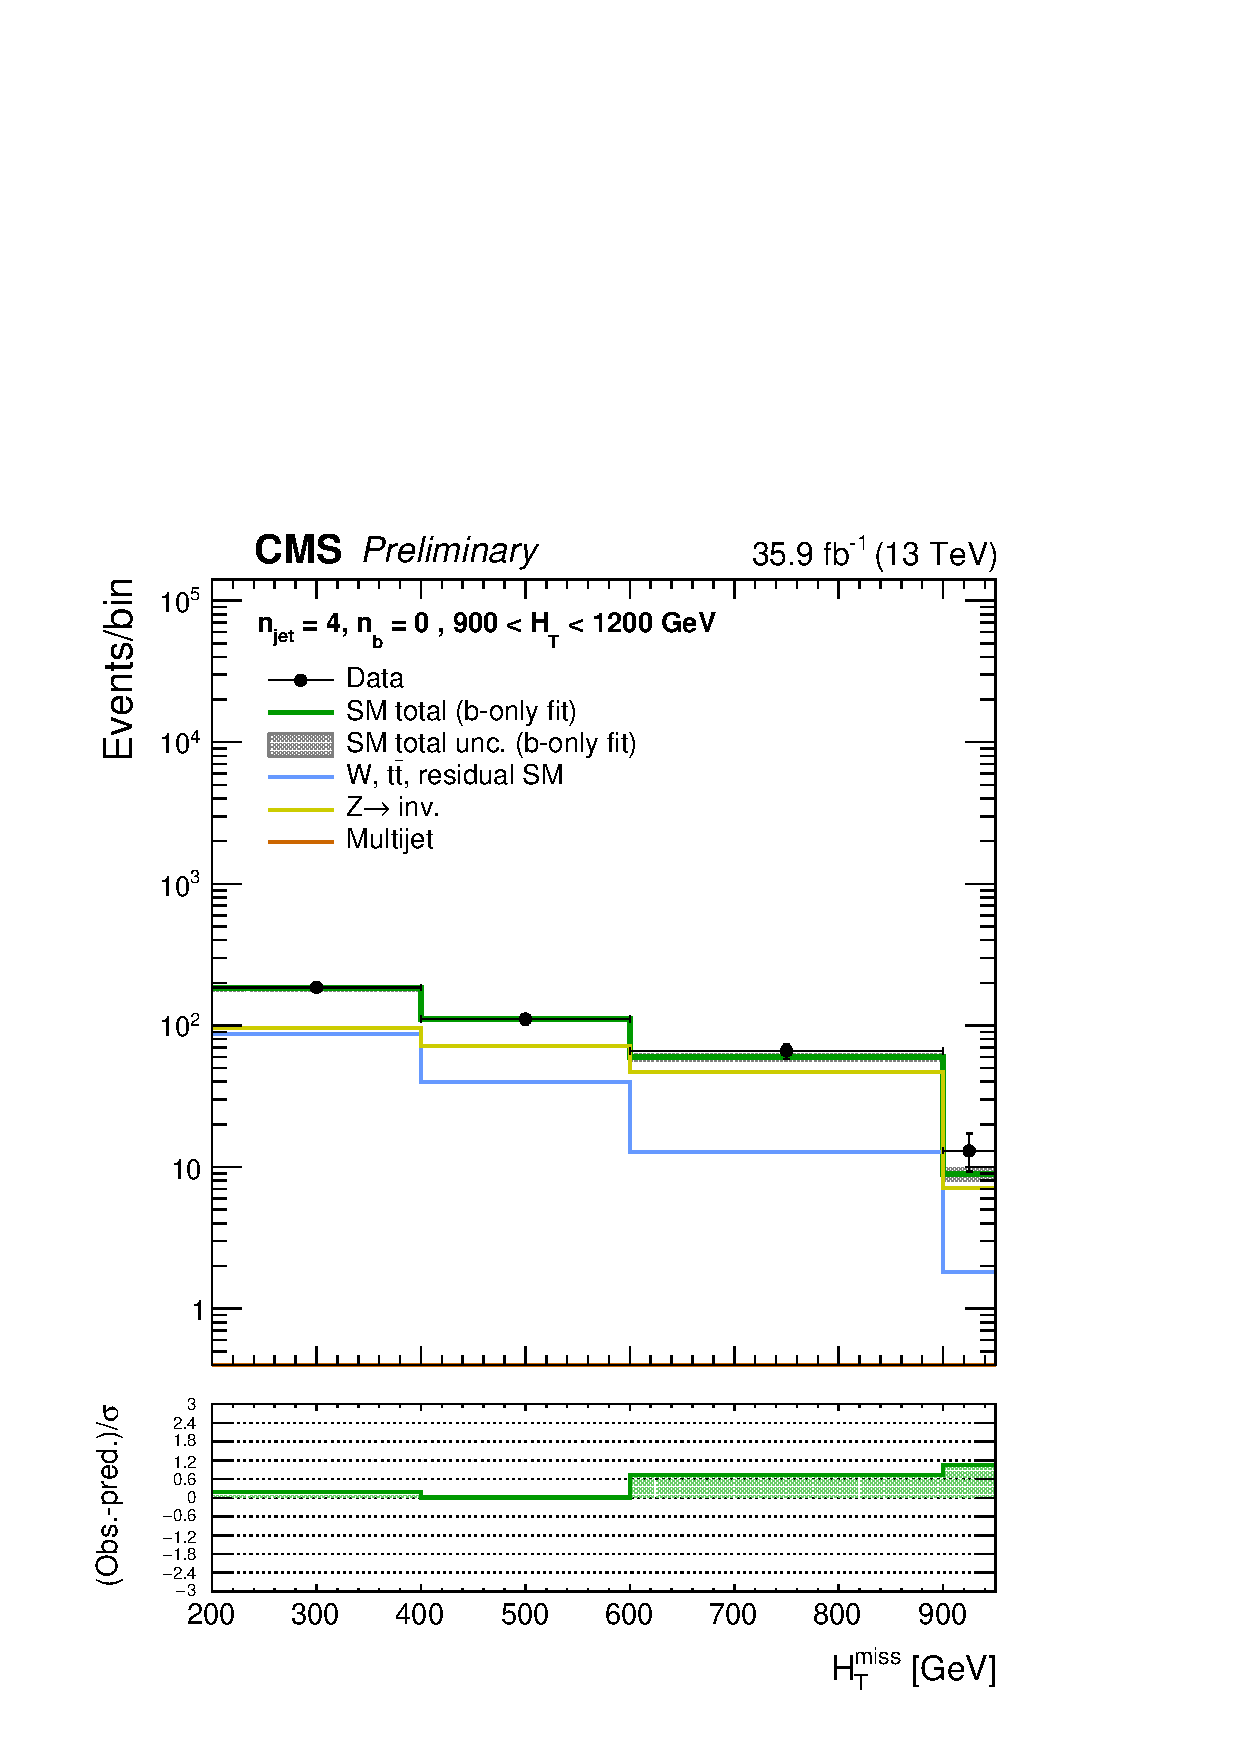
\includegraphics[width=0.49\textwidth]{figures/results/36invfb//crfit/shapes//mhtShape_eq0b_eq4j_900_1200_fit_b.pdf}}
    \subfigure[$\scalht > 1200\GeV$]{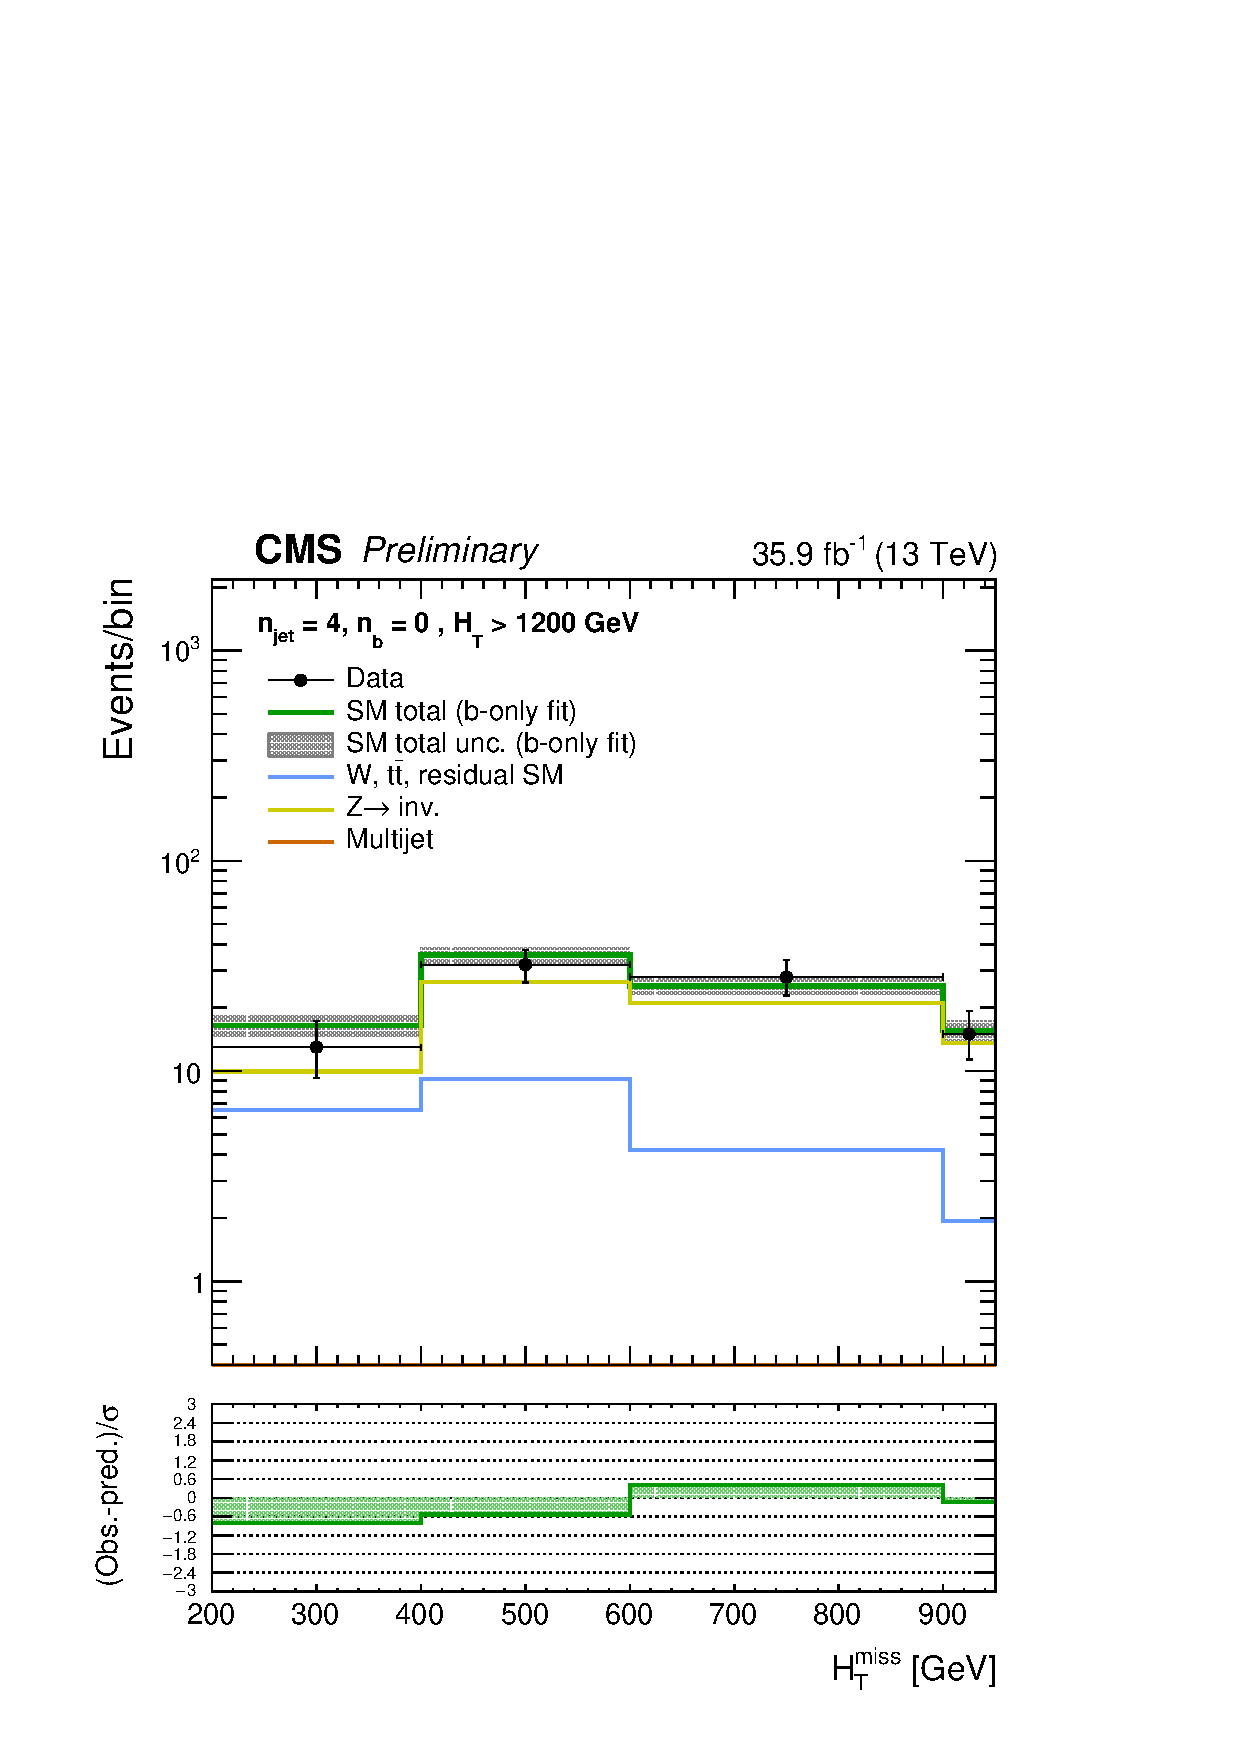
\includegraphics[width=0.49\textwidth]{figures/results/36invfb//crfit/shapes//mhtShape_eq0b_eq4j_1200_Inf_fit_b.pdf}}\\
    \caption{Event yields observed in data (solid circles) and CR-fit SM expectations with their associated uncertainties (green histogram with shaded band) as a function of \HTmiss based on a sample of events that satisfy $\njet = 4$ and $\nb = 0$, as well as the requirements on \scalht indicated by each sub-figure caption. }
    \label{fig:mhtval_eq4j_eq0b}
  \end{center}
\end{figure}

\begin{figure}[h!]
  \begin{center}
    \subfigure[$400 < \scalht < 600\GeV$]{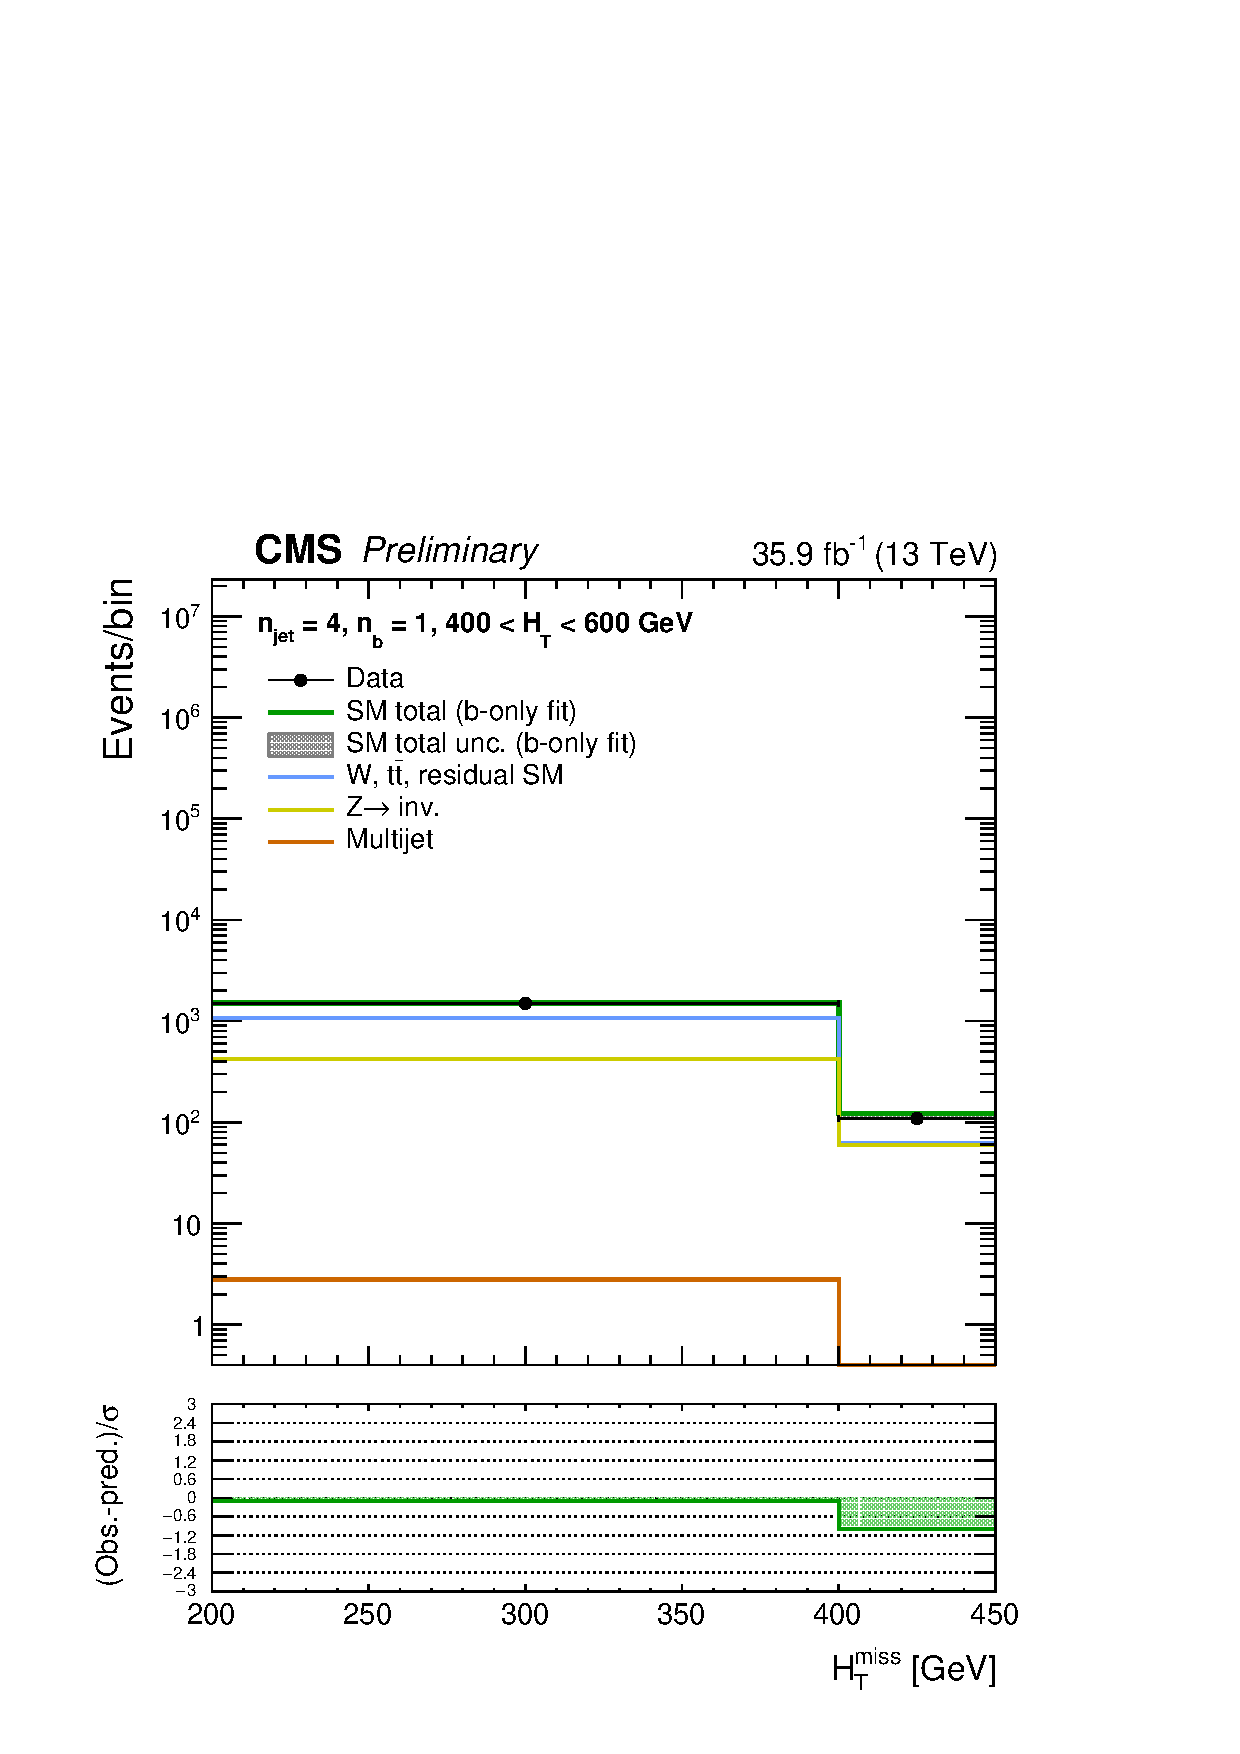
\includegraphics[width=0.49\textwidth]{figures/results/36invfb//crfit/shapes//mhtShape_eq1b_eq4j_400_600_fit_b.pdf}}
    \subfigure[$600 < \scalht < 900\GeV$]{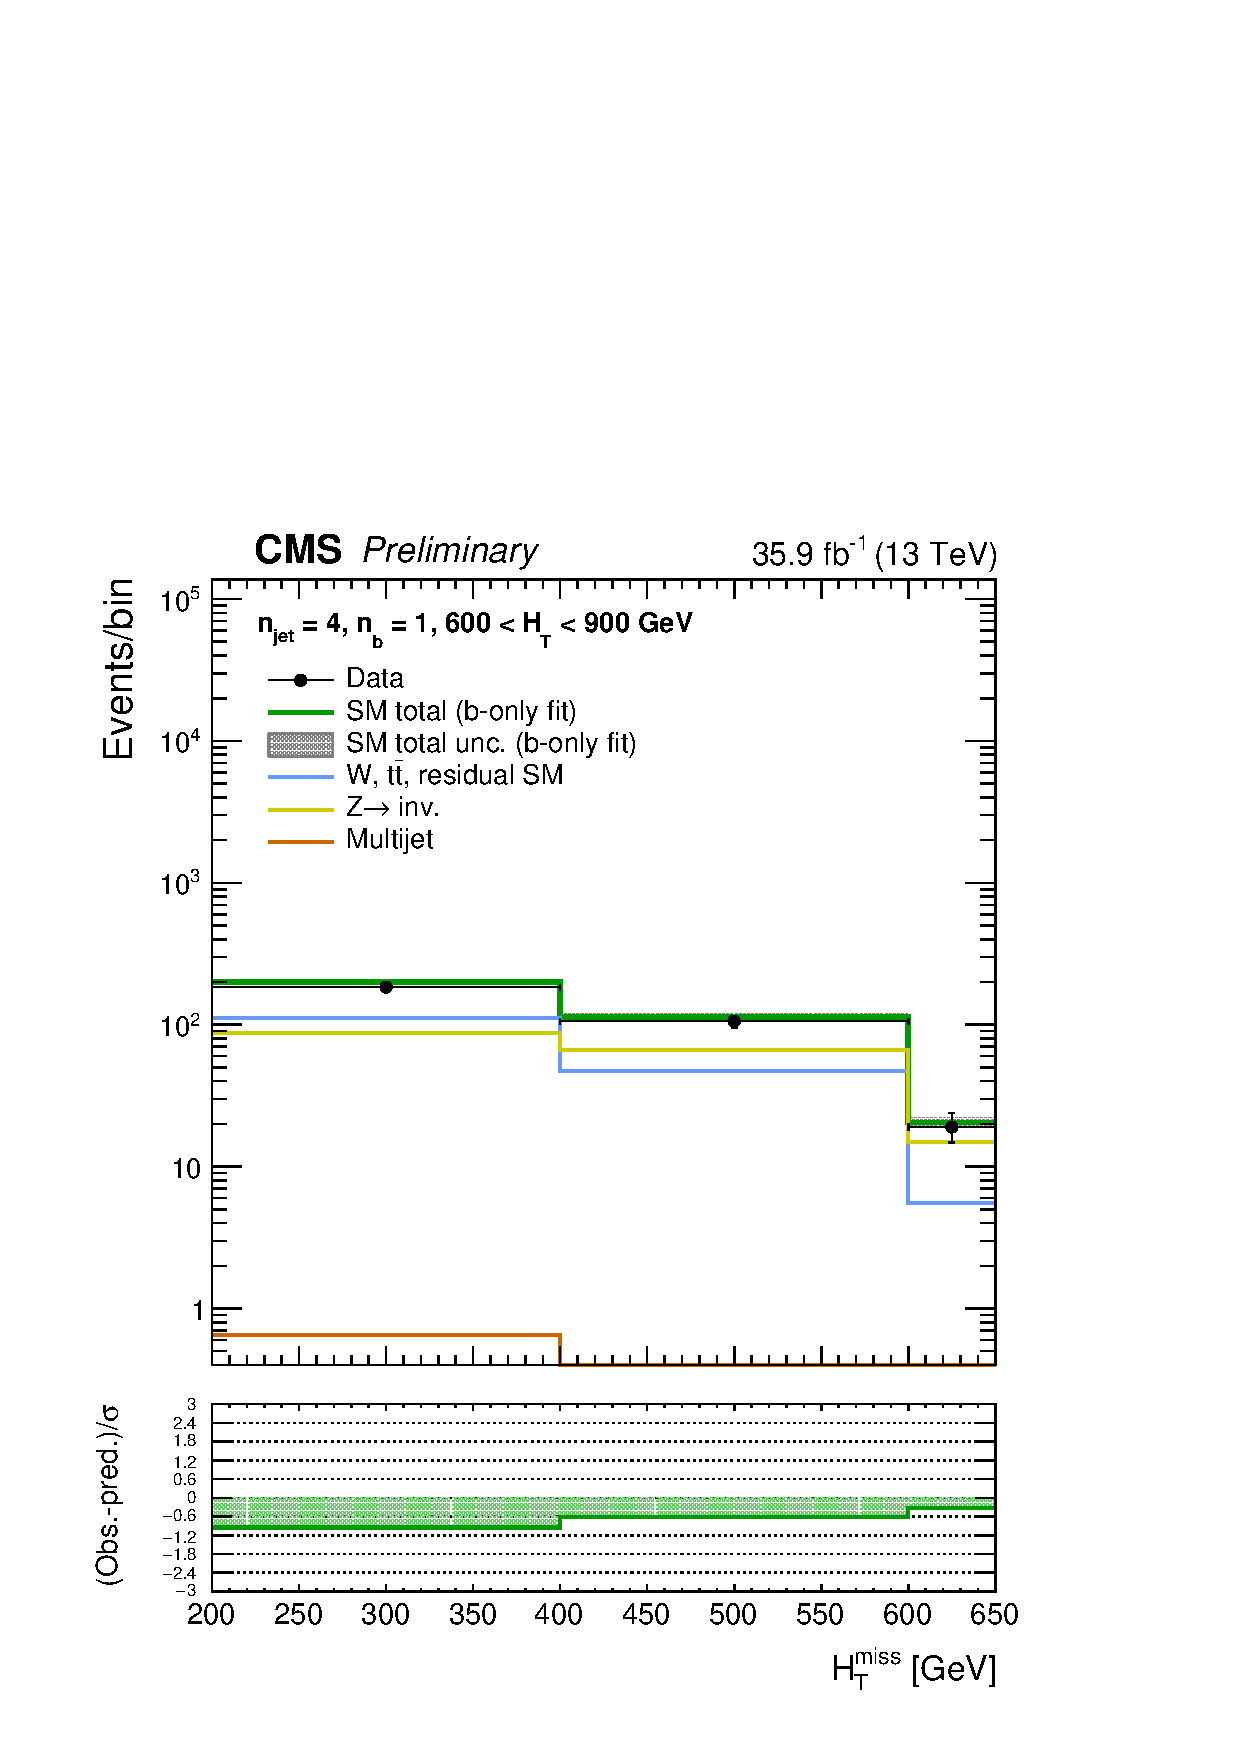
\includegraphics[width=0.49\textwidth]{figures/results/36invfb//crfit/shapes//mhtShape_eq1b_eq4j_600_900_fit_b.pdf}}\\
    \subfigure[$900 < \scalht < 1200\GeV$]{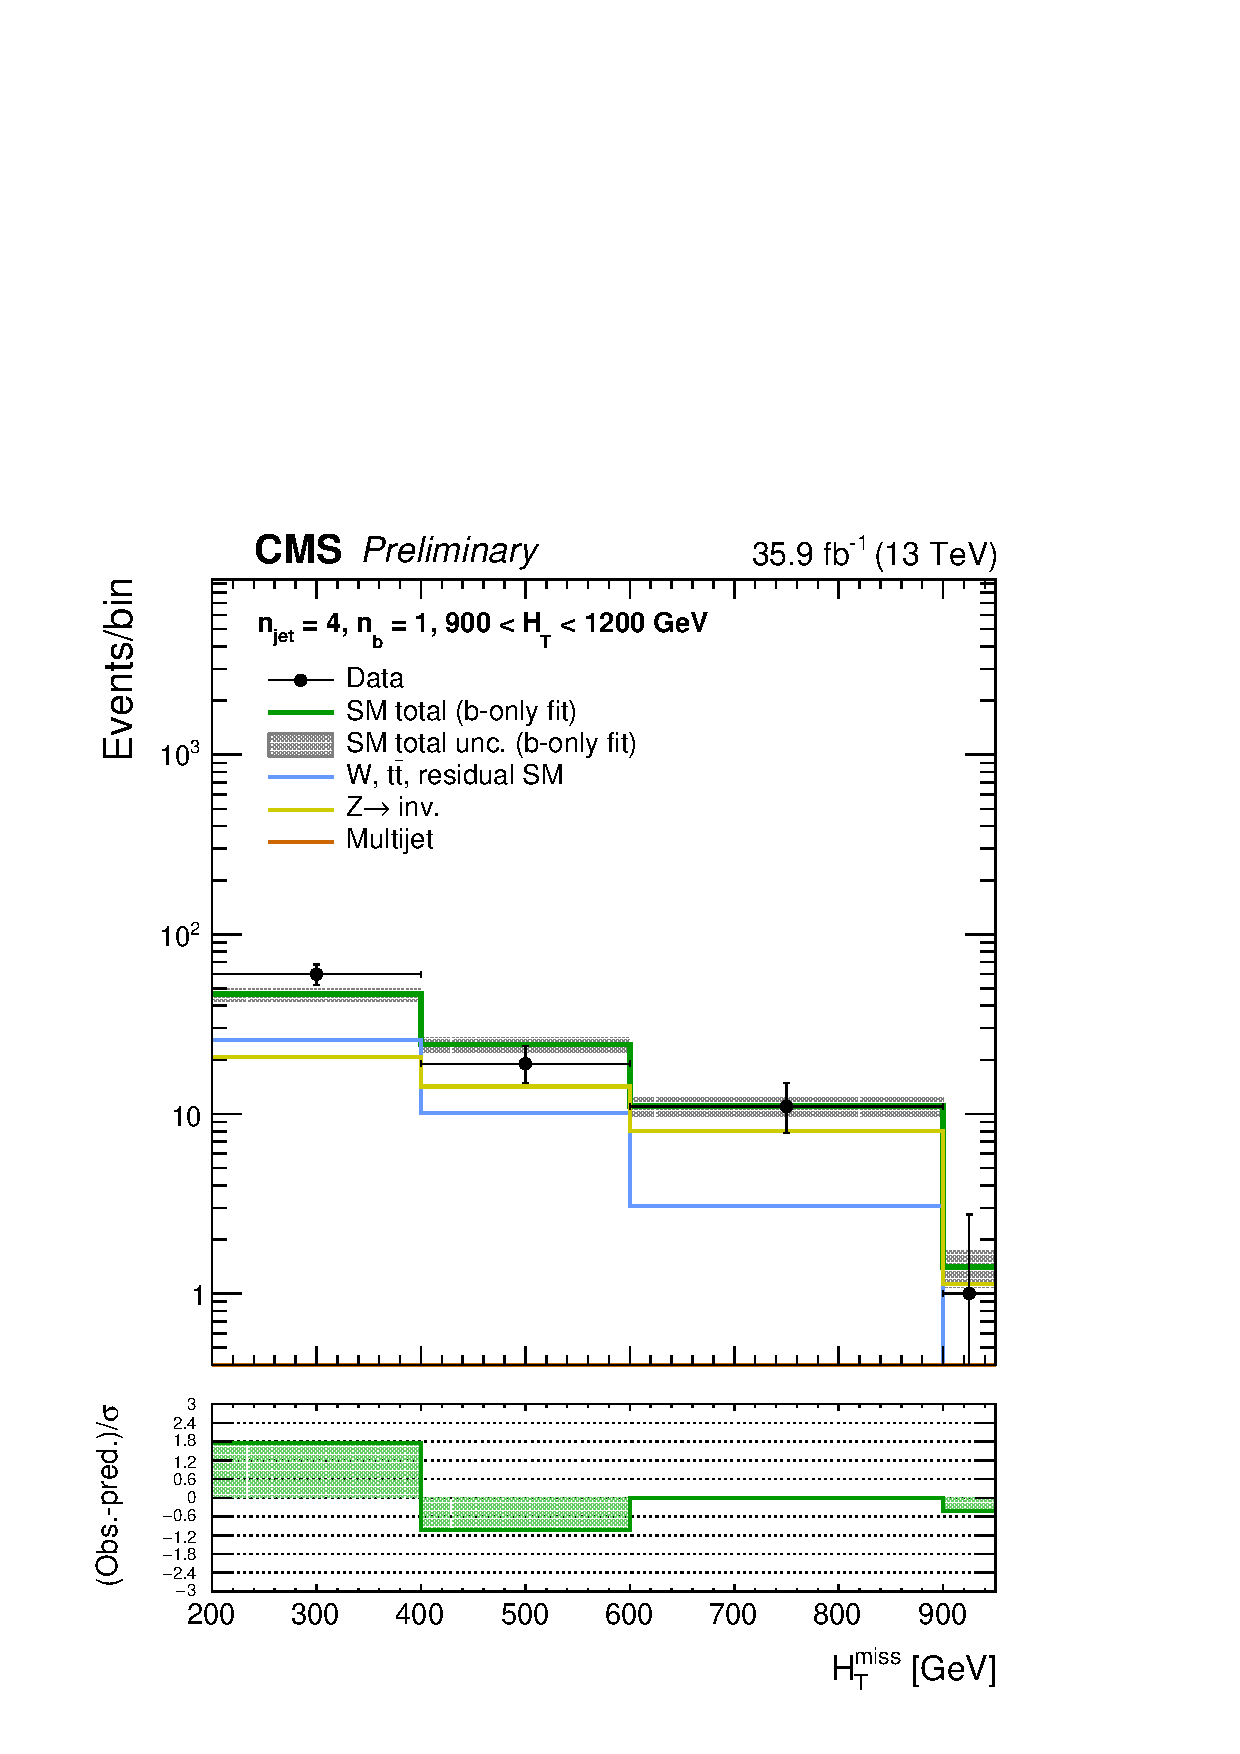
\includegraphics[width=0.49\textwidth]{figures/results/36invfb//crfit/shapes//mhtShape_eq1b_eq4j_900_1200_fit_b.pdf}}
    \subfigure[$\scalht > 1200\GeV$]{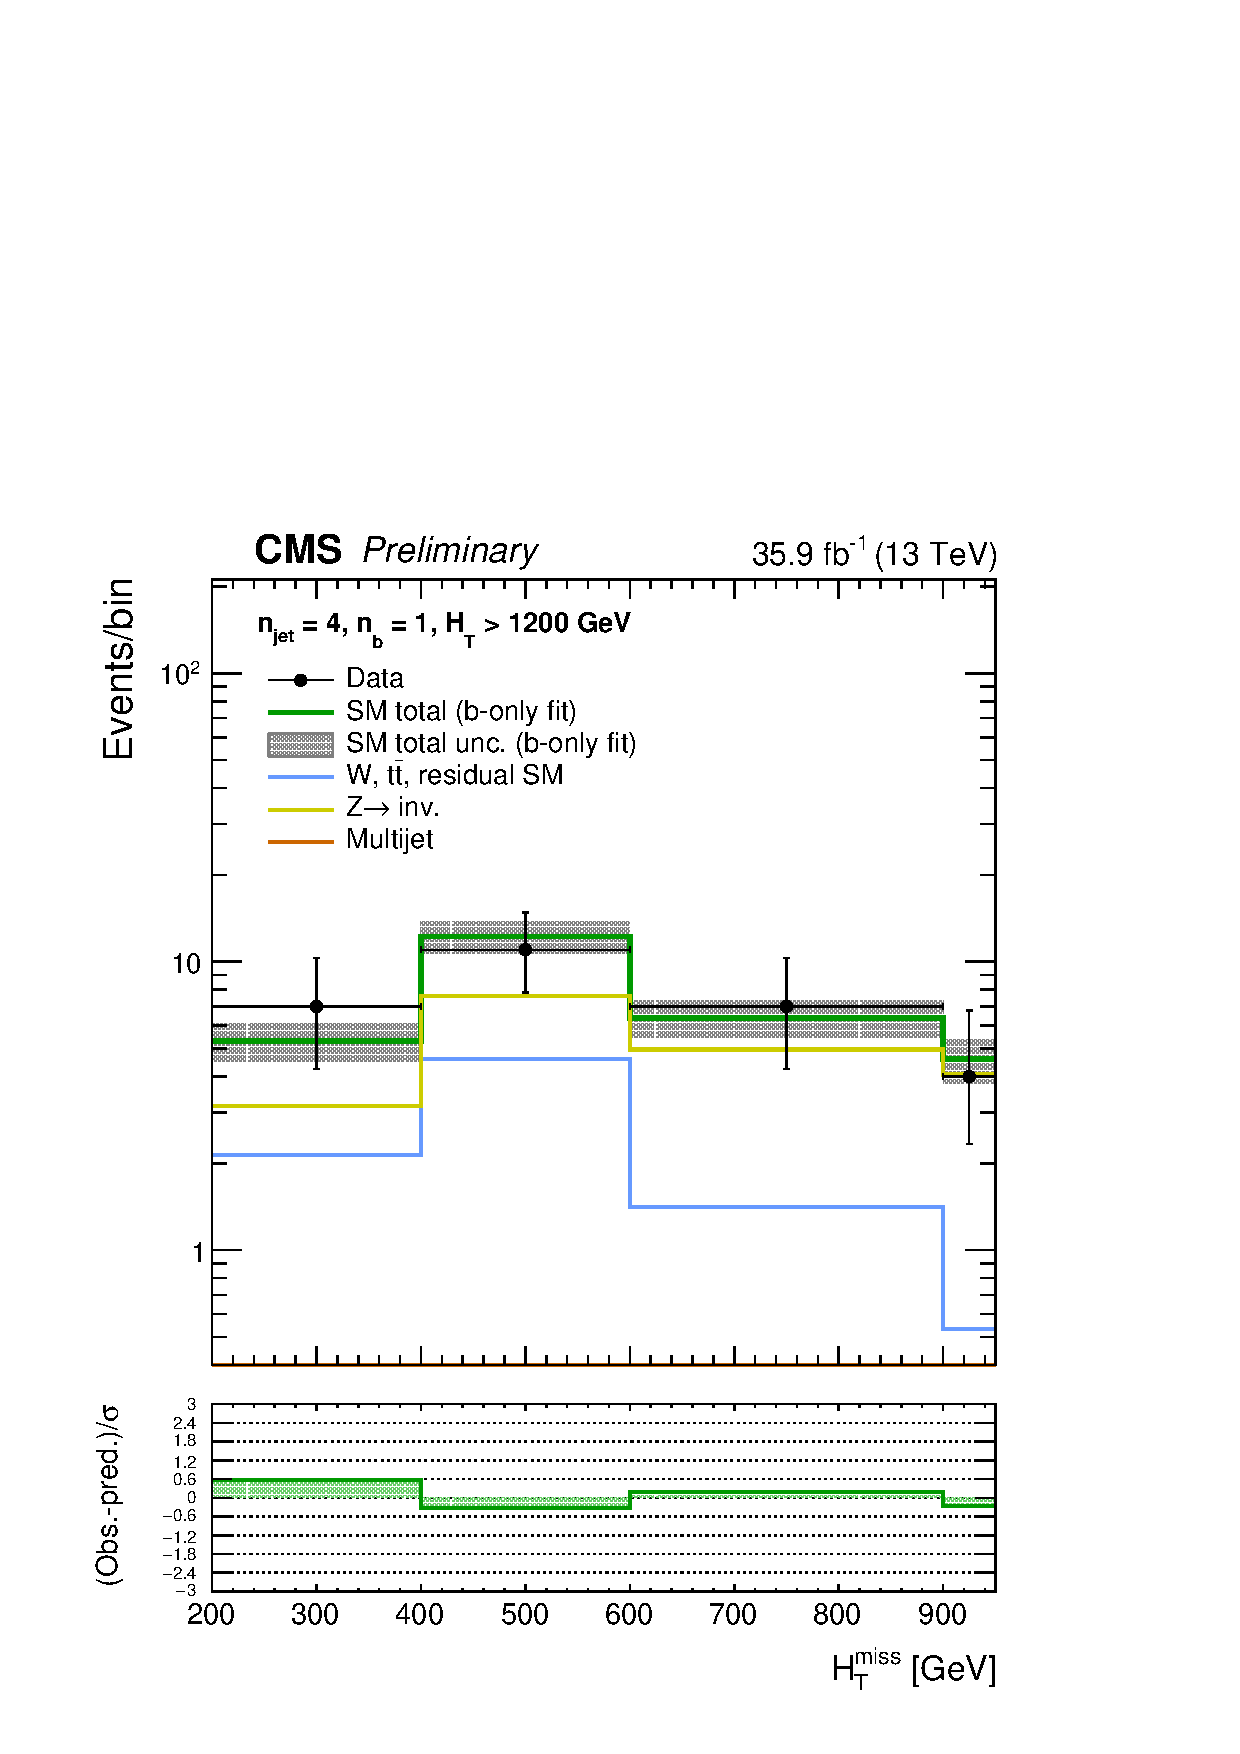
\includegraphics[width=0.49\textwidth]{figures/results/36invfb//crfit/shapes//mhtShape_eq1b_eq4j_1200_Inf_fit_b.pdf}}\\
    \caption{Event yields observed in data (solid circles) and CR-fit SM expectations with their associated uncertainties (green histogram with shaded band) as a function of \HTmiss based on a sample of events that satisfy $\njet = 4$ and $\nb = 1$, as well as the requirements on \scalht indicated by each sub-figure caption. }
    \label{fig:mhtval_eq4j_eq1b}
  \end{center}
\end{figure}

\begin{figure}[h!]
  \begin{center}
    \subfigure[$400 < \scalht < 600\GeV$]{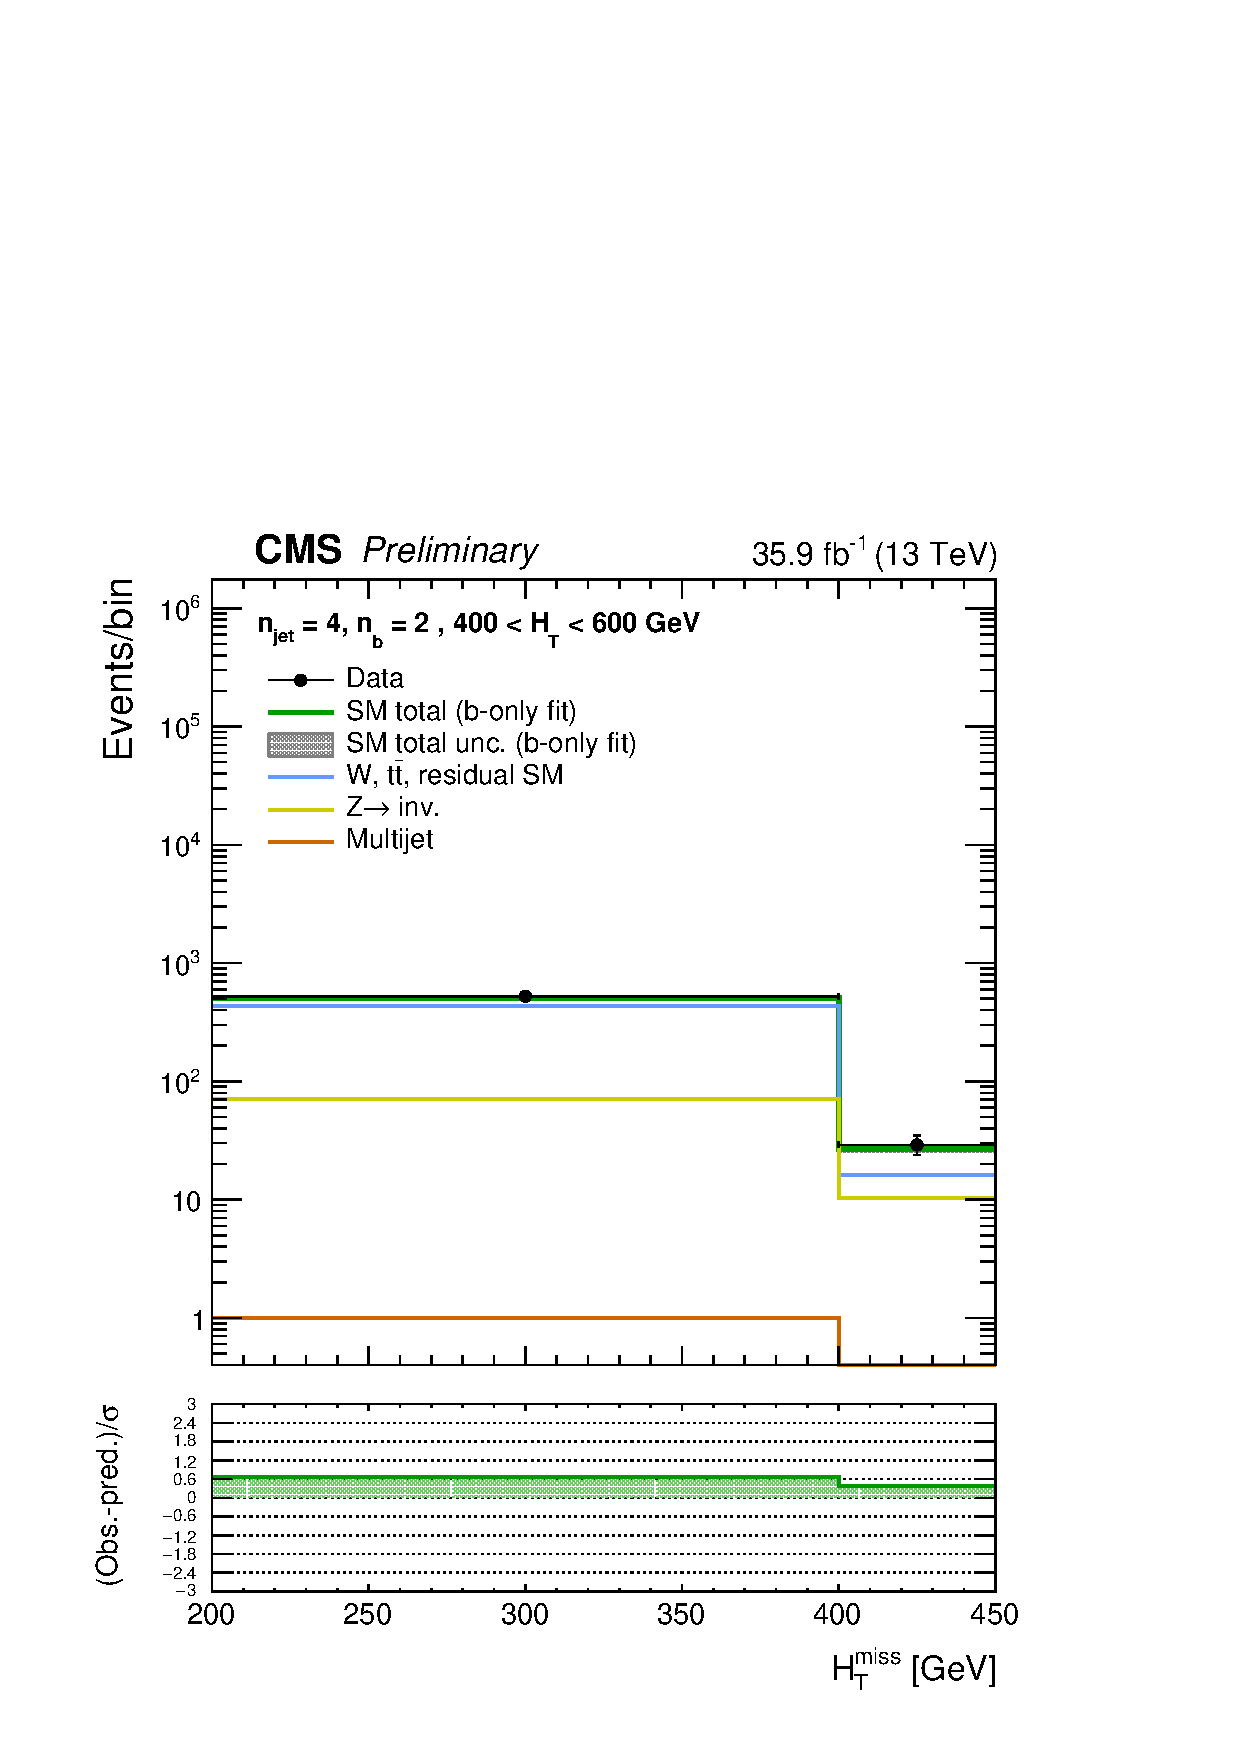
\includegraphics[width=0.49\textwidth]{figures/results/36invfb//crfit/shapes//mhtShape_eq2b_eq4j_400_600_fit_b.pdf}}
    \subfigure[$600 < \scalht < 900\GeV$]{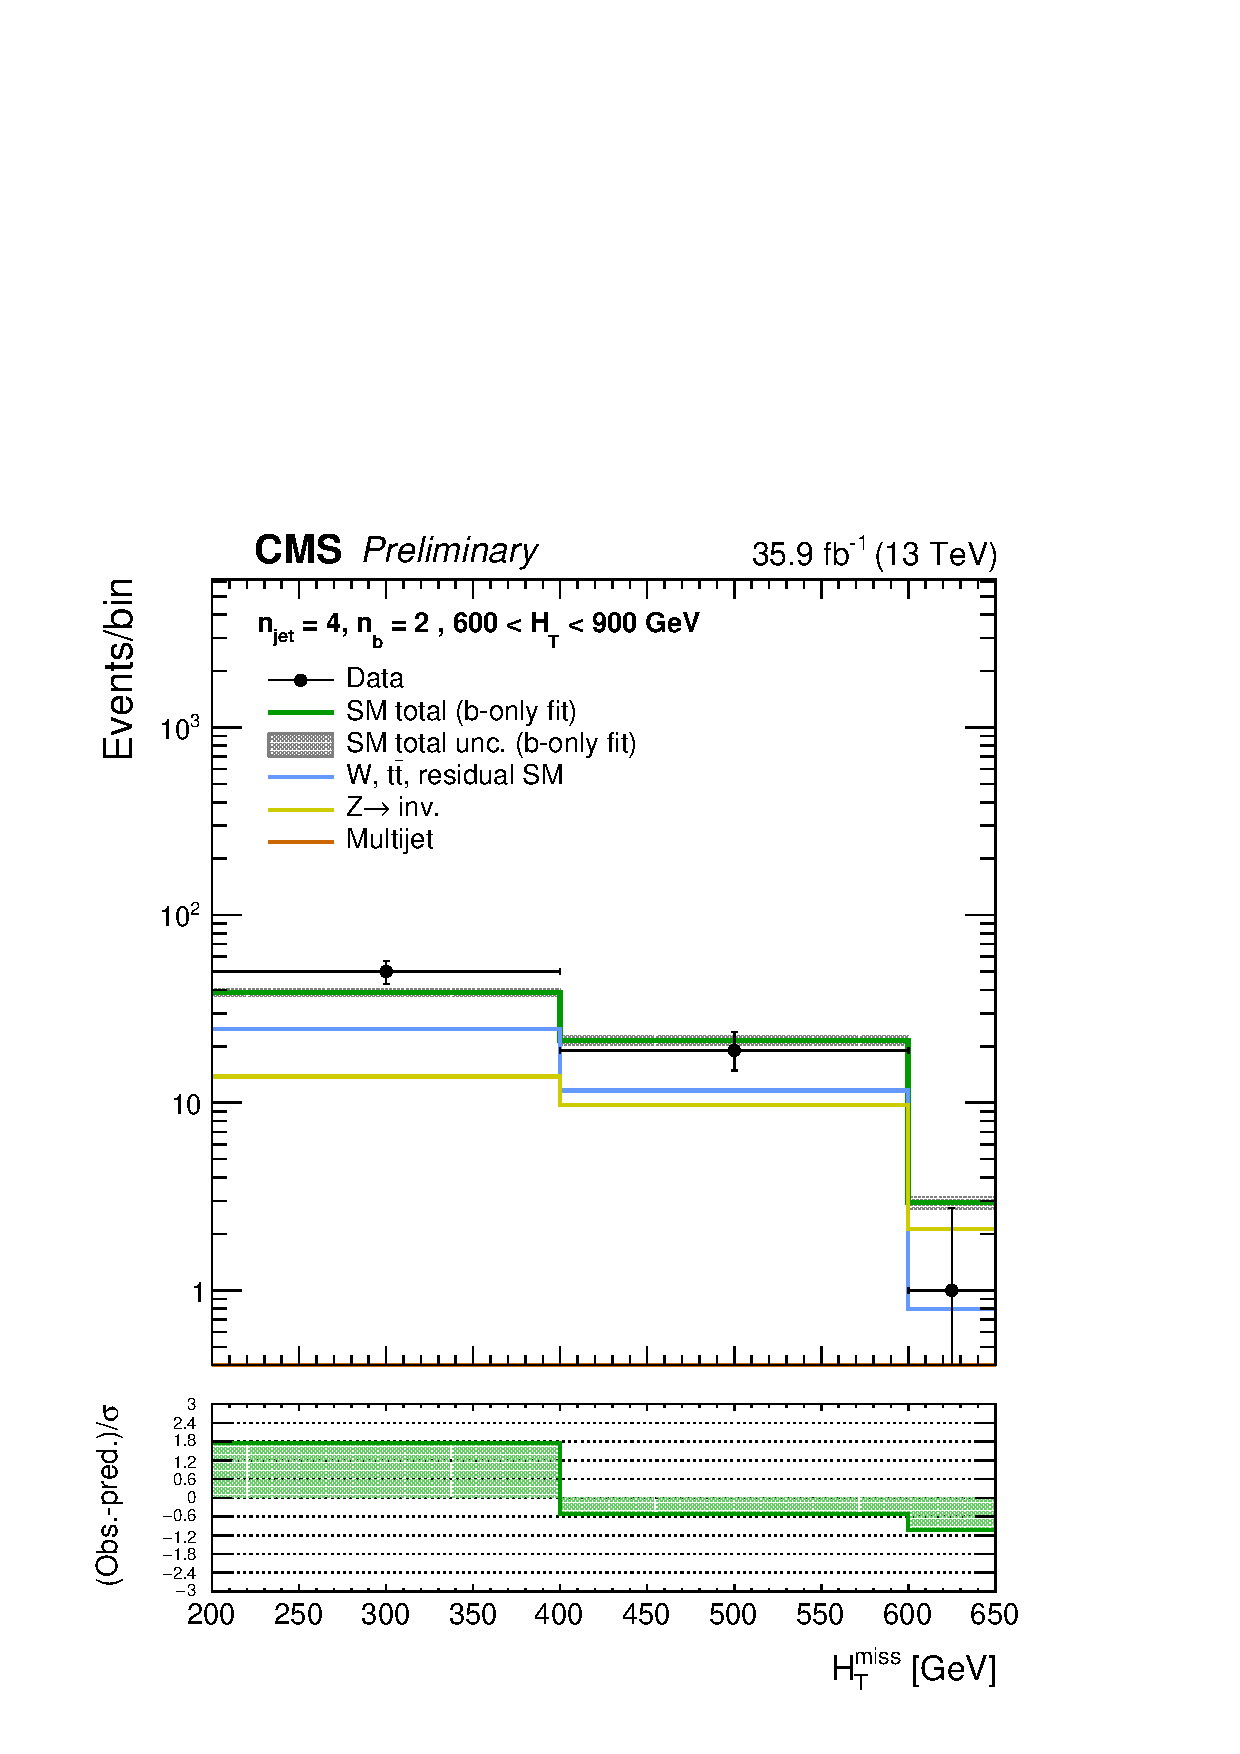
\includegraphics[width=0.49\textwidth]{figures/results/36invfb//crfit/shapes//mhtShape_eq2b_eq4j_600_900_fit_b.pdf}}\\
    \subfigure[$900 < \scalht < 1200\GeV$]{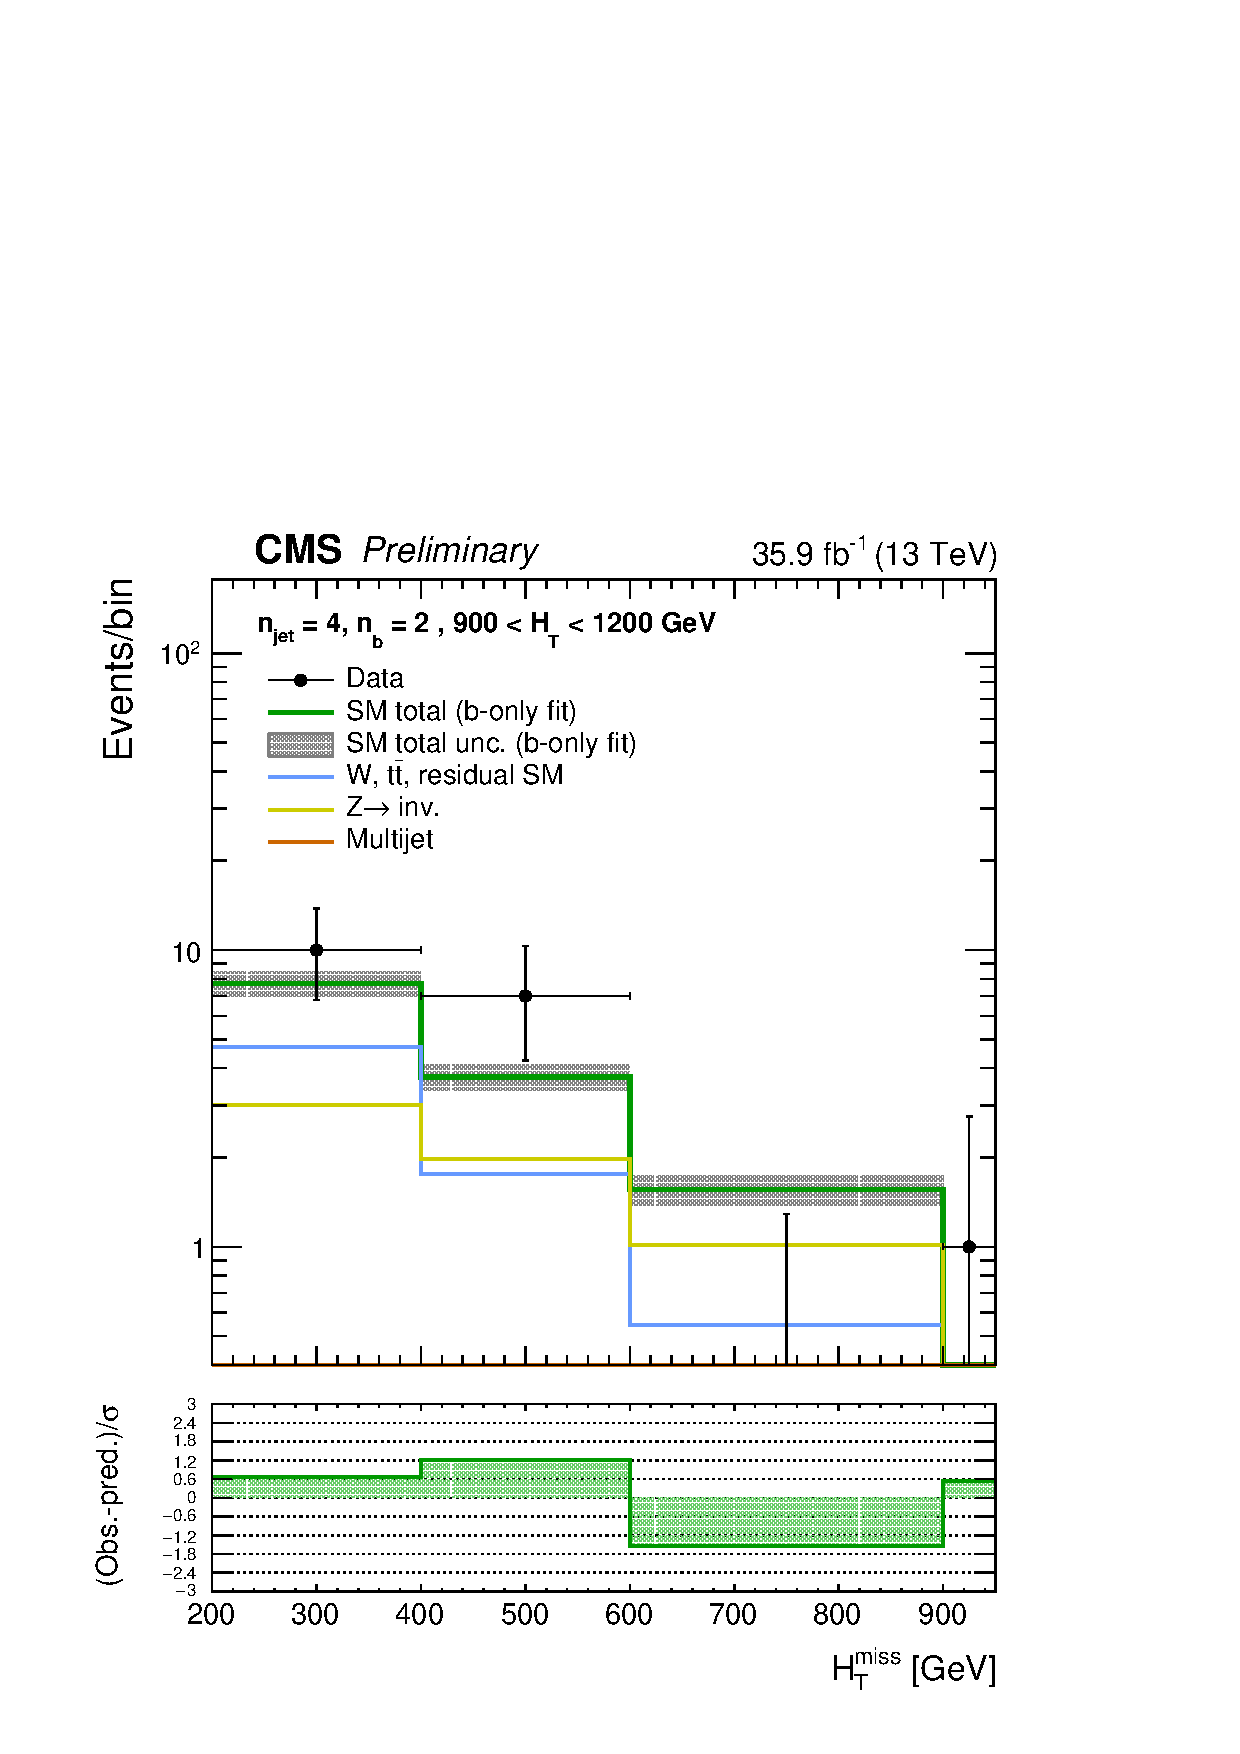
\includegraphics[width=0.49\textwidth]{figures/results/36invfb//crfit/shapes//mhtShape_eq2b_eq4j_900_1200_fit_b.pdf}}
    \subfigure[$\scalht > 1200\GeV$]{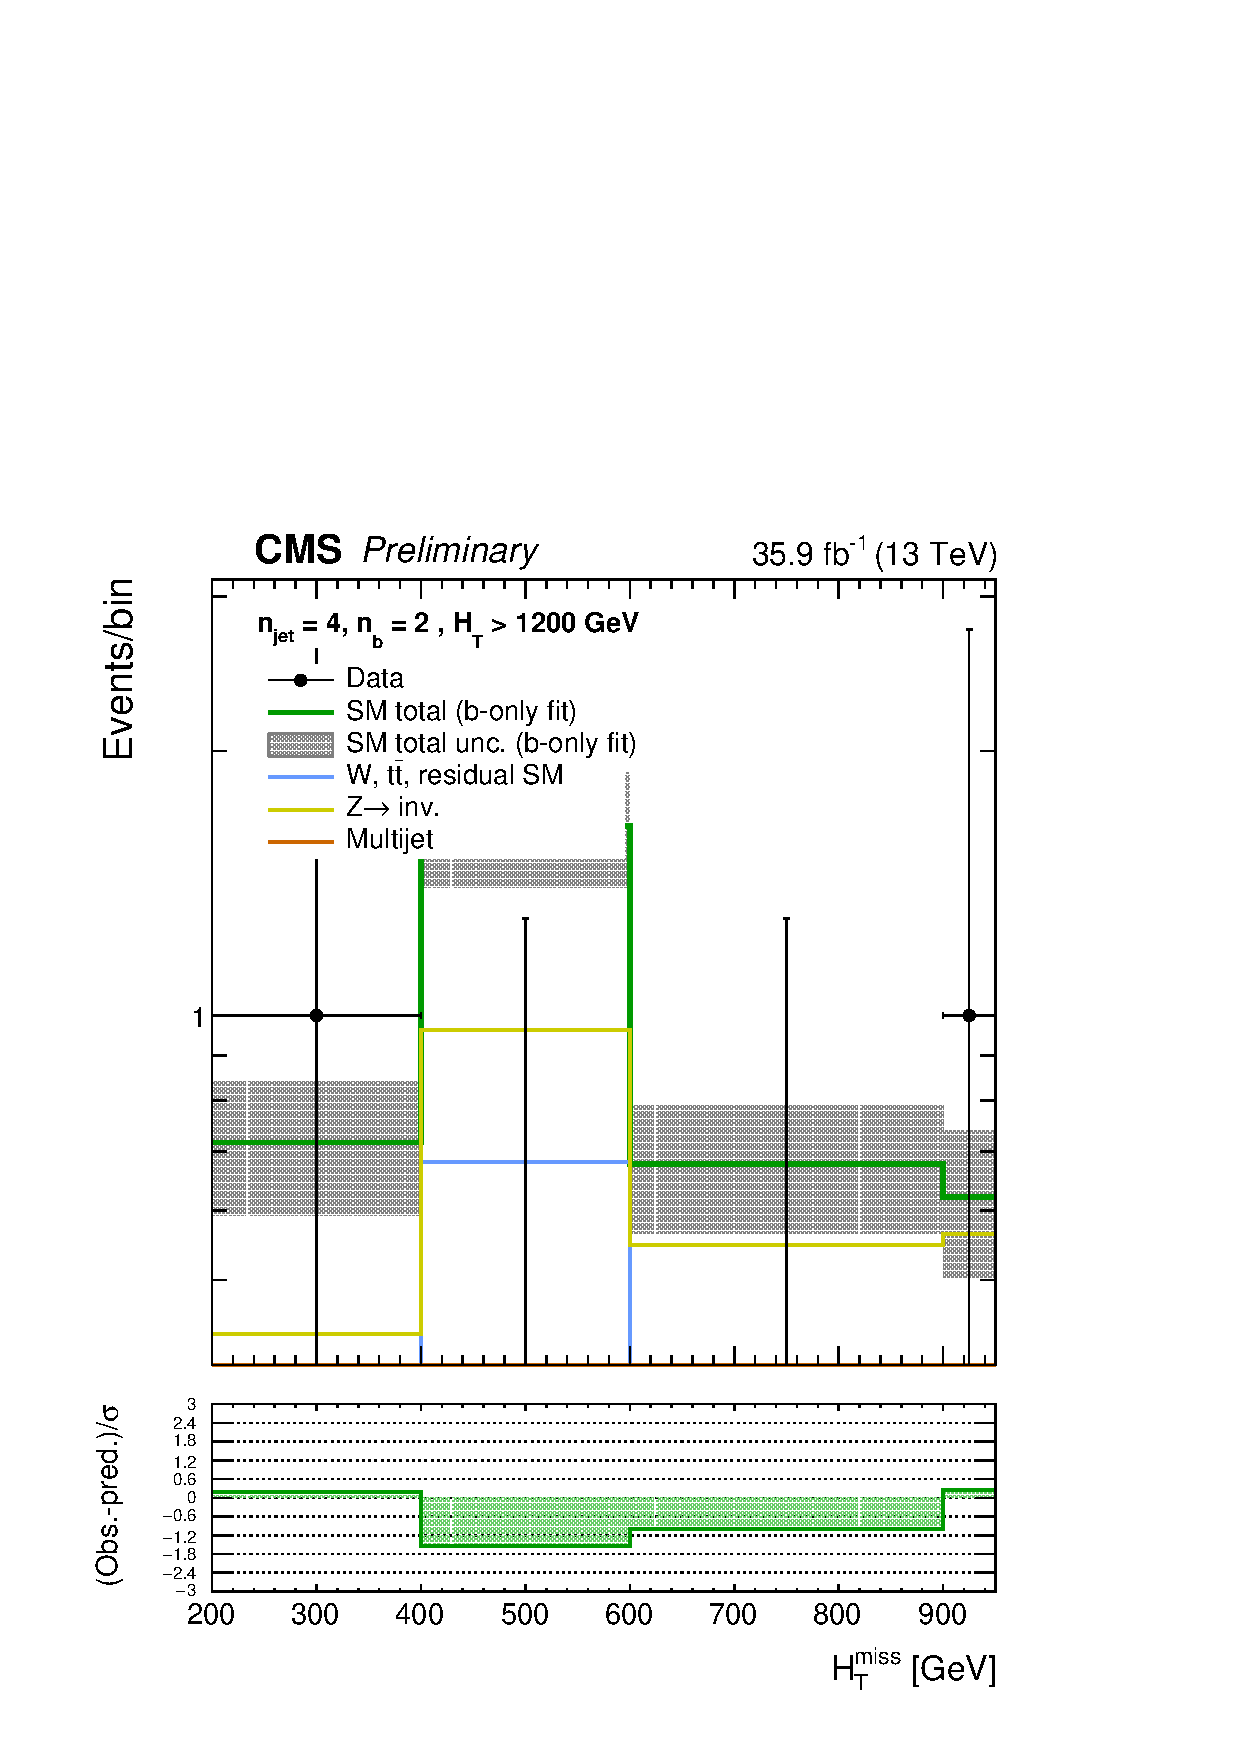
\includegraphics[width=0.49\textwidth]{figures/results/36invfb//crfit/shapes//mhtShape_eq2b_eq4j_1200_Inf_fit_b.pdf}}\\
    \caption{Event yields observed in data (solid circles) and CR-fit SM expectations with their associated uncertainties (green histogram with shaded band) as a function of \HTmiss based on a sample of events that satisfy $\njet = 4$ and $\nb = 2$, as well as the requirements on \scalht indicated by each sub-figure caption. }
    \label{fig:mhtval_eq4j_eq2b}
  \end{center}
\end{figure}

\begin{figure}[h!]
  \begin{center}
    \subfigure[$400 < \scalht < 600\GeV$]{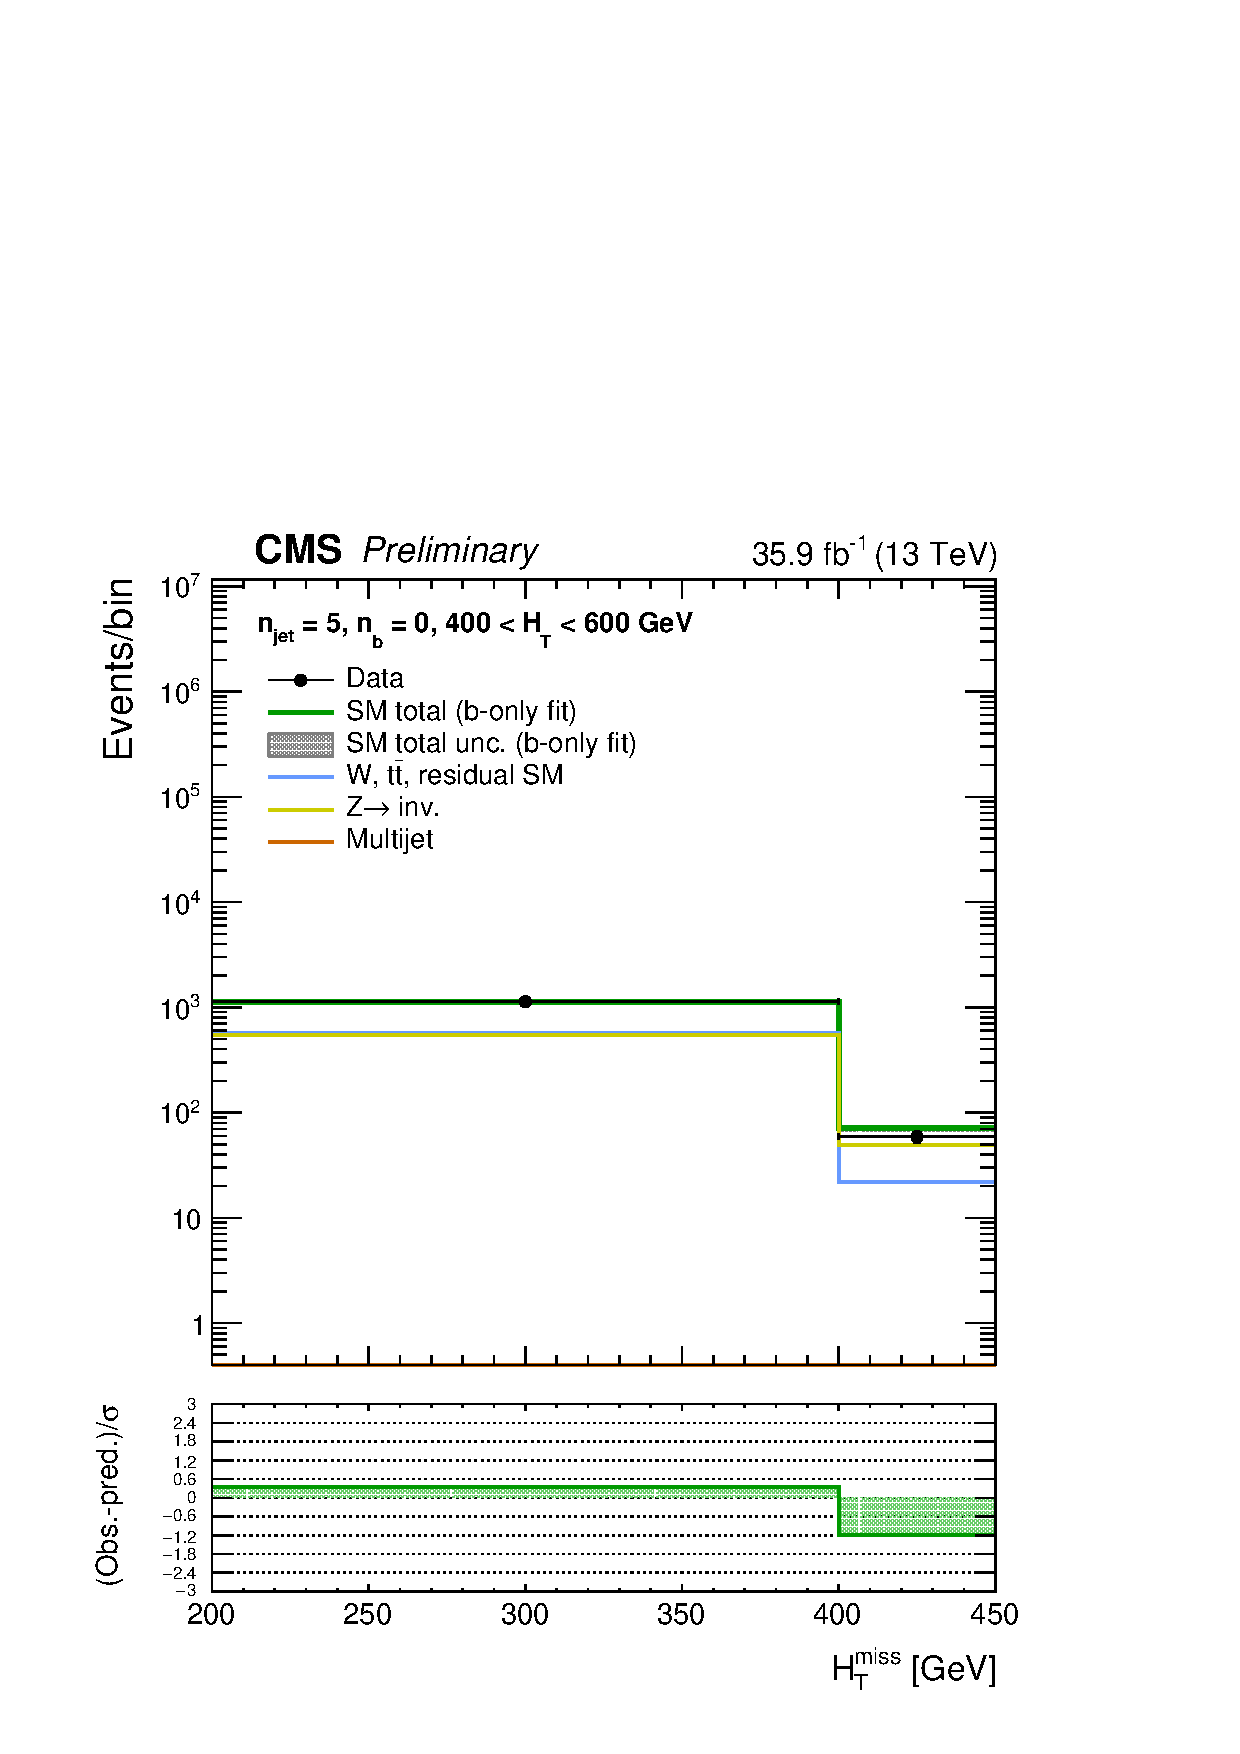
\includegraphics[width=0.49\textwidth]{figures/results/36invfb//crfit/shapes//mhtShape_eq0b_eq5j_400_600_fit_b.pdf}}
    \subfigure[$600 < \scalht < 900\GeV$]{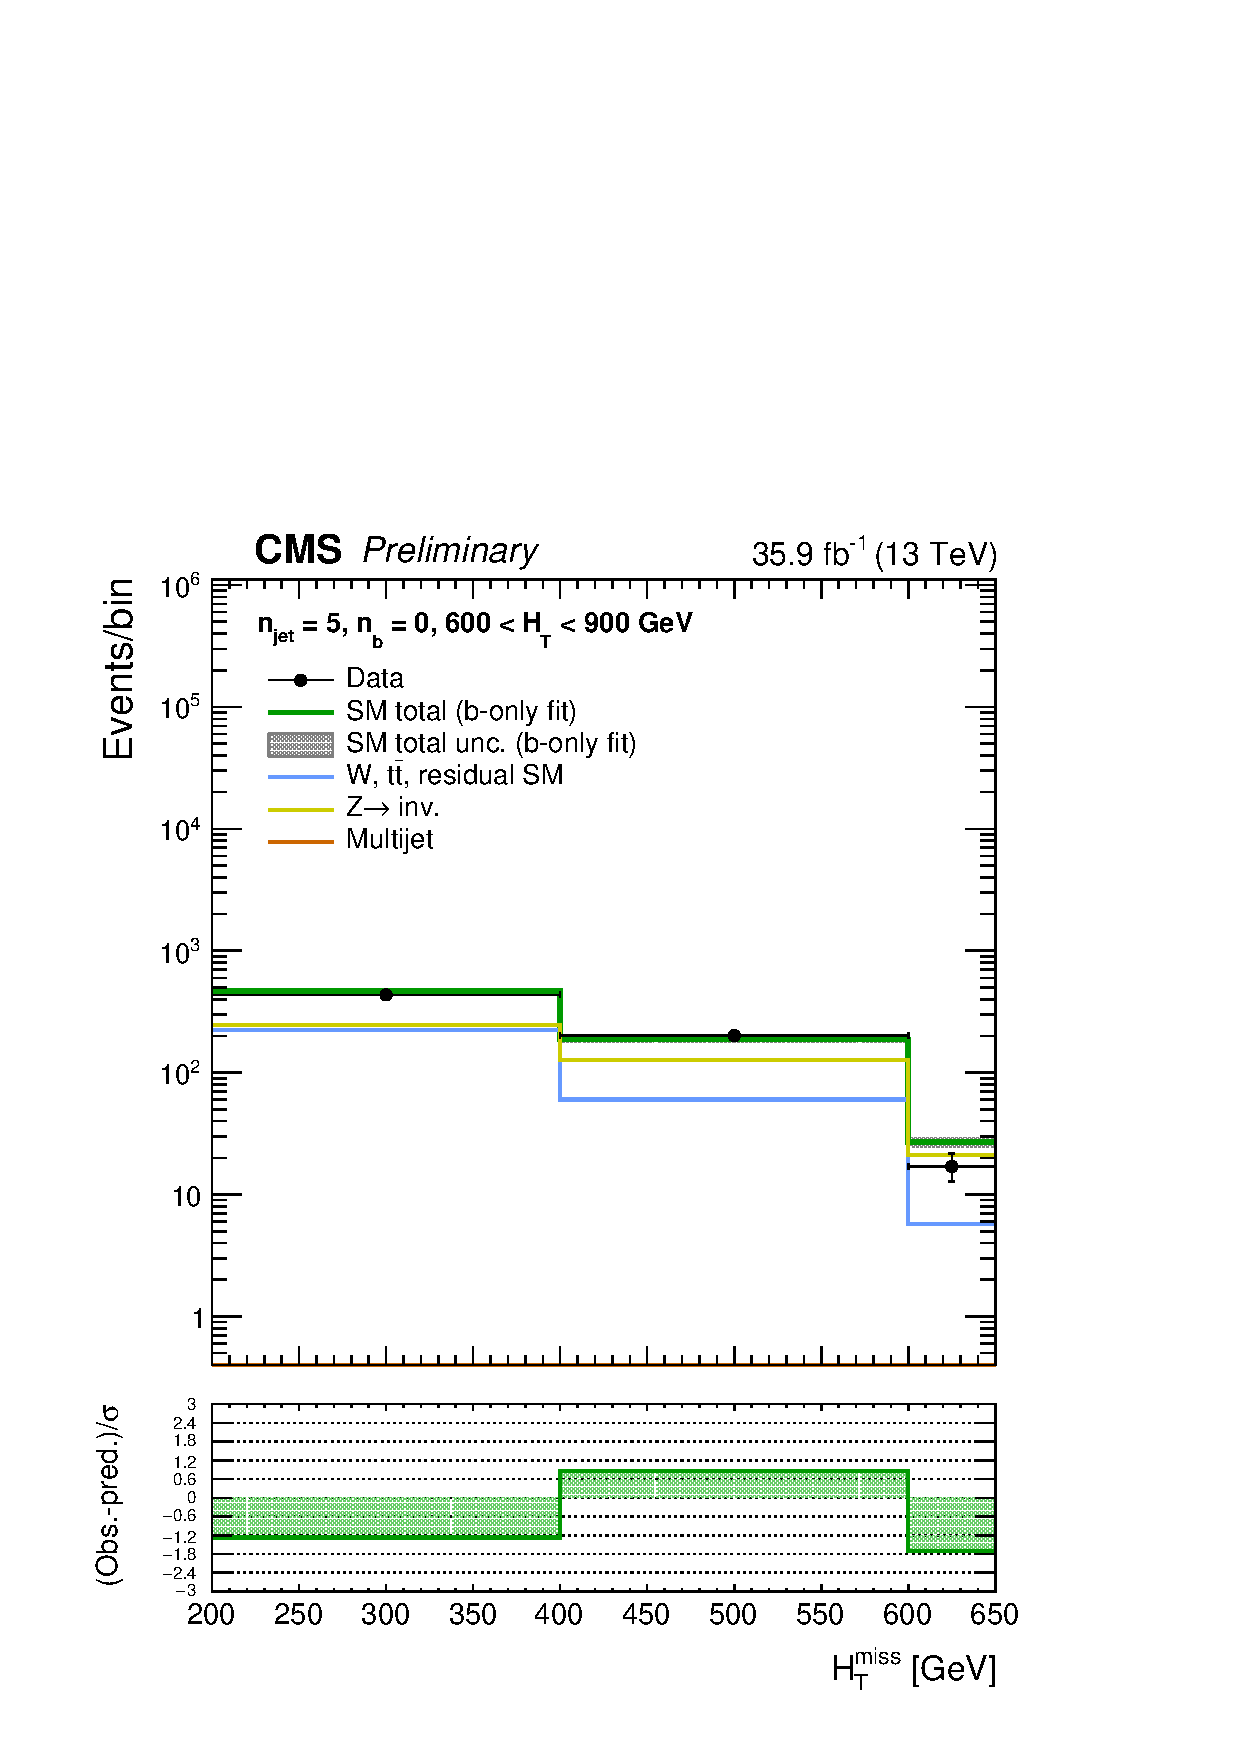
\includegraphics[width=0.49\textwidth]{figures/results/36invfb//crfit/shapes//mhtShape_eq0b_eq5j_600_900_fit_b.pdf}}\\
    \subfigure[$900 < \scalht < 1200\GeV$]{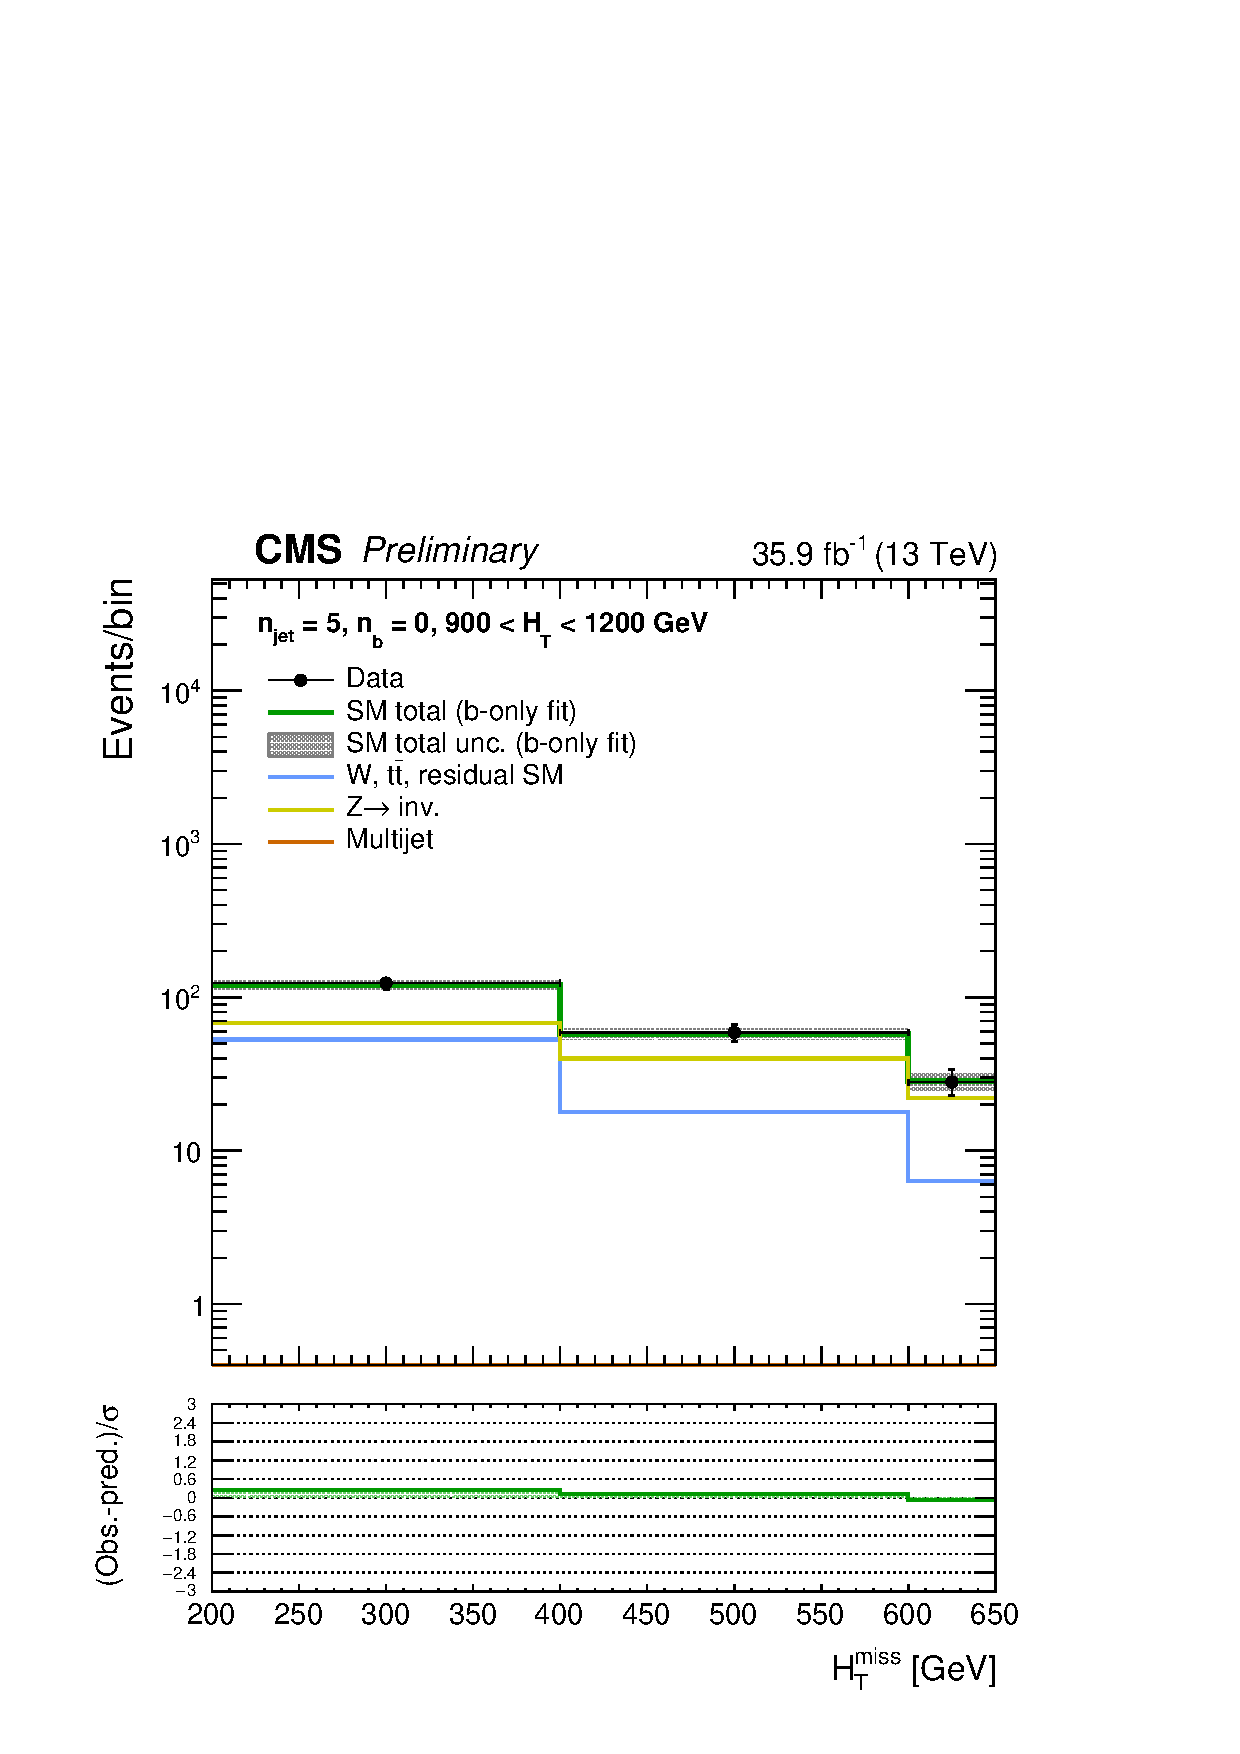
\includegraphics[width=0.49\textwidth]{figures/results/36invfb//crfit/shapes//mhtShape_eq0b_eq5j_900_1200_fit_b.pdf}}
    \subfigure[$\scalht > 1200\GeV$]{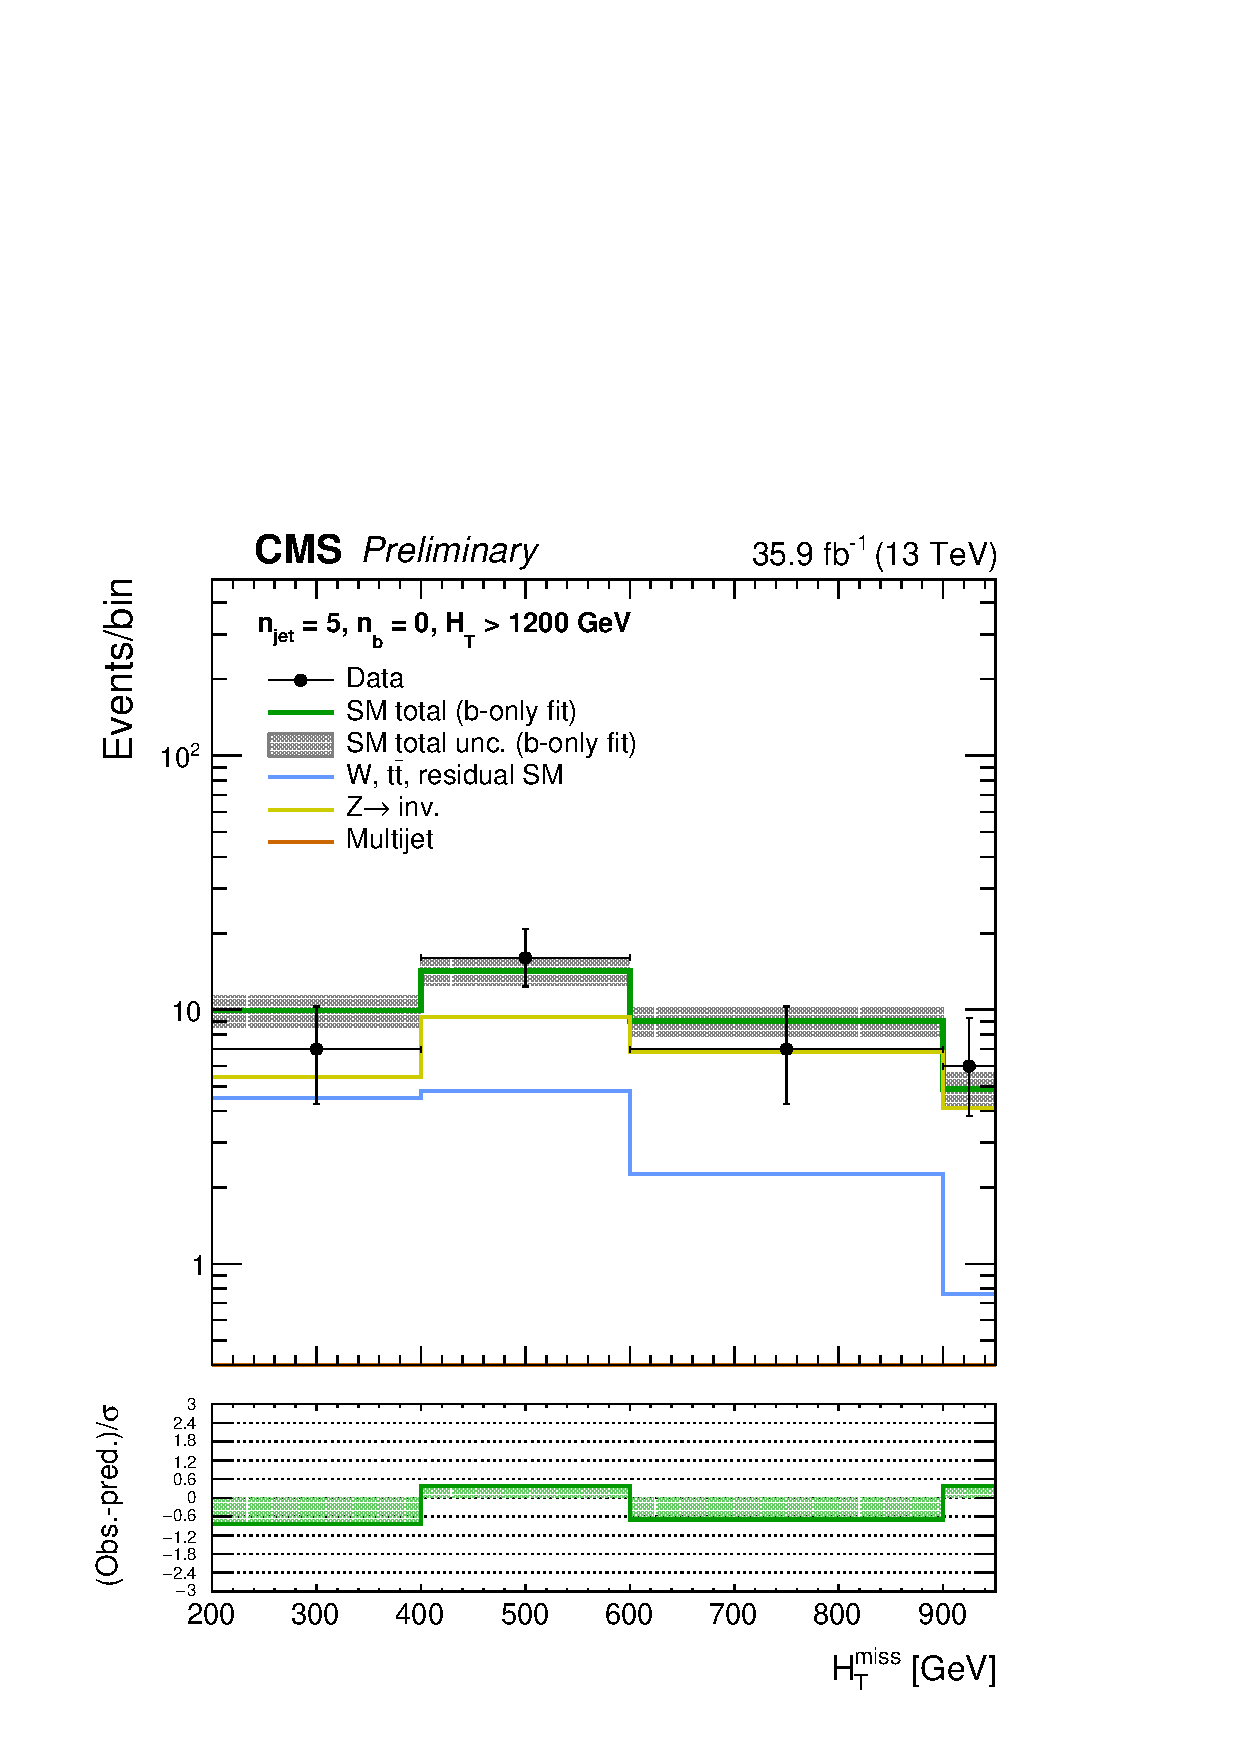
\includegraphics[width=0.49\textwidth]{figures/results/36invfb//crfit/shapes//mhtShape_eq0b_eq5j_1200_Inf_fit_b.pdf}}\\
    \caption{Event yields observed in data (solid circles) and CR-fit SM expectations with their associated uncertainties (green histogram with shaded band) as a function of \HTmiss based on a sample of events that satisfy $\njet = 5$ and $\nb = 0$, as well as the requirements on \scalht indicated by each sub-figure caption. }
    \label{fig:mhtval_eq5j_eq0b}
  \end{center}
\end{figure}

\begin{figure}[h!]
  \begin{center}
    \subfigure[$400 < \scalht < 600\GeV$]{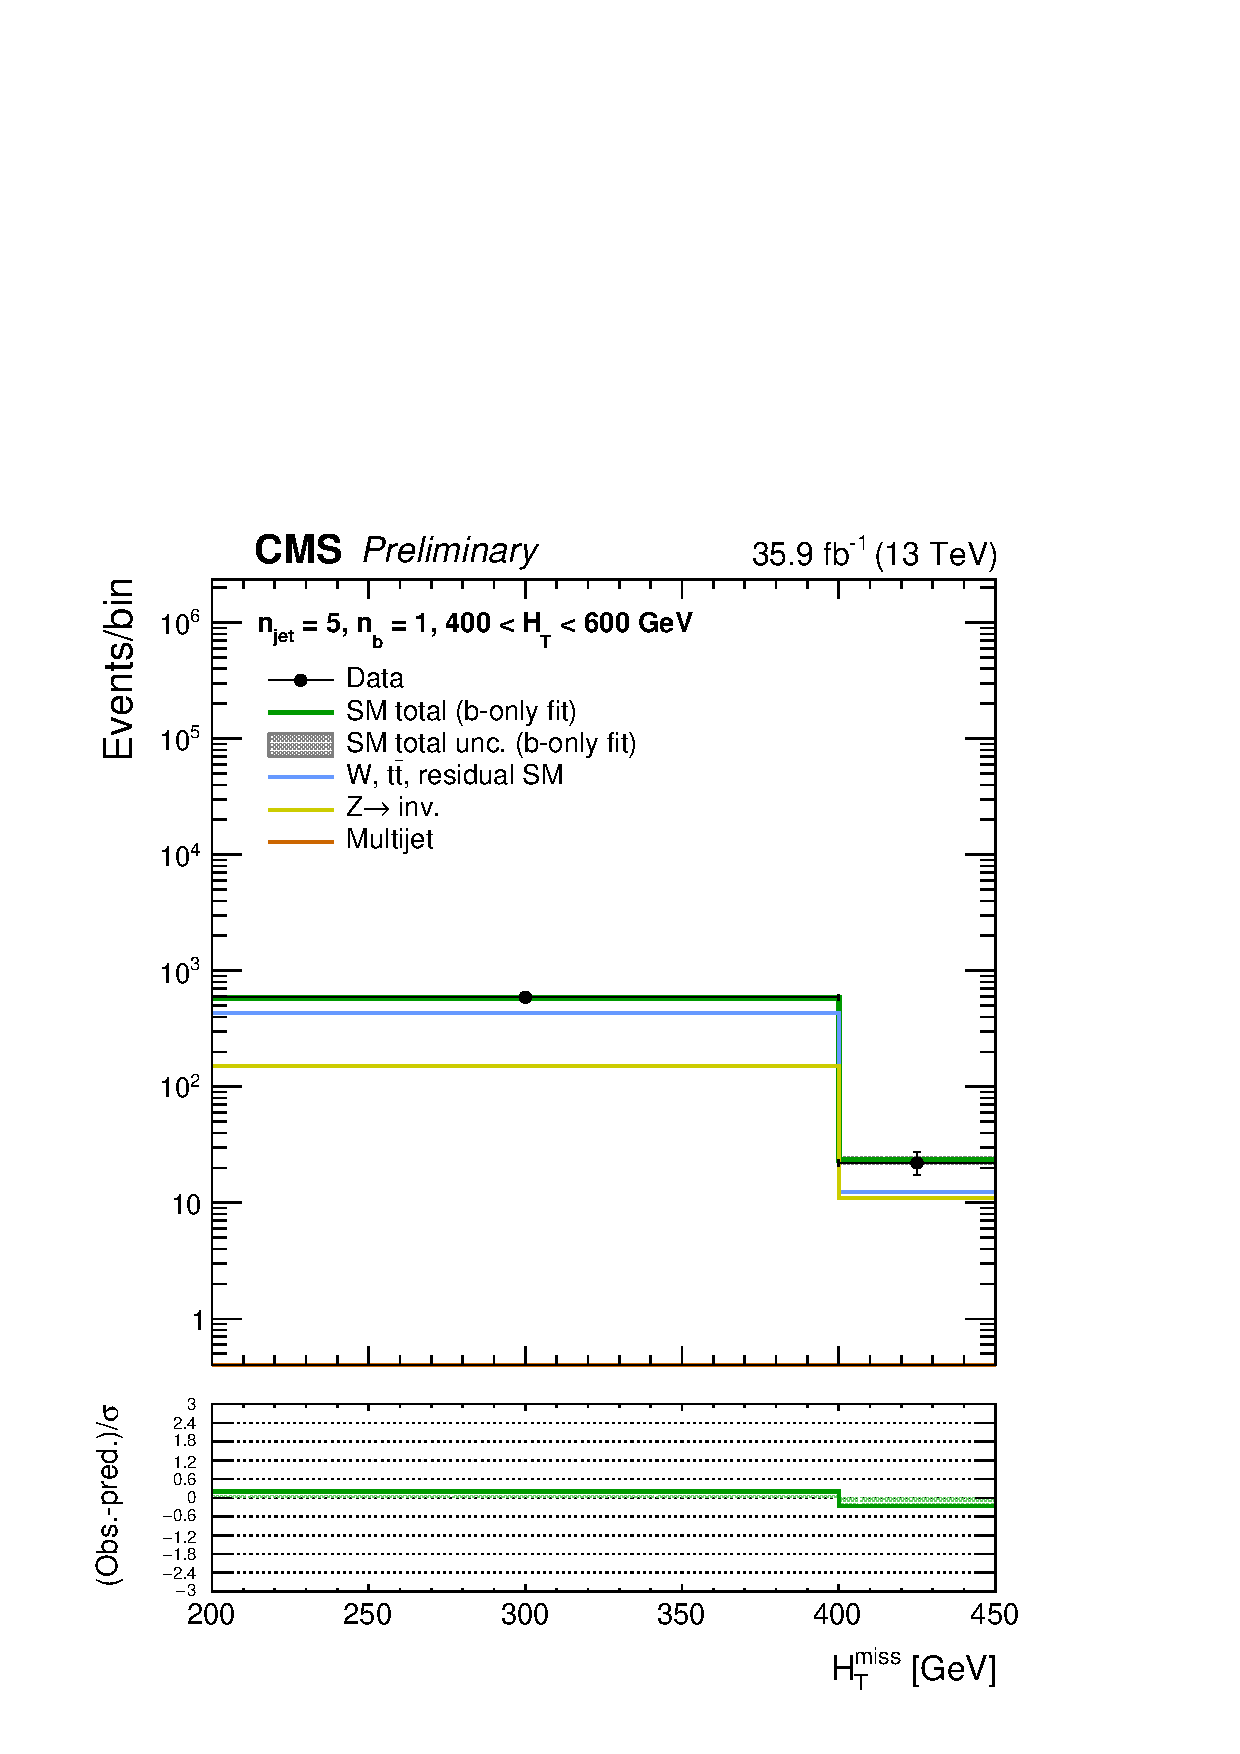
\includegraphics[width=0.49\textwidth]{figures/results/36invfb//crfit/shapes//mhtShape_eq1b_eq5j_400_600_fit_b.pdf}}
    \subfigure[$600 < \scalht < 900\GeV$]{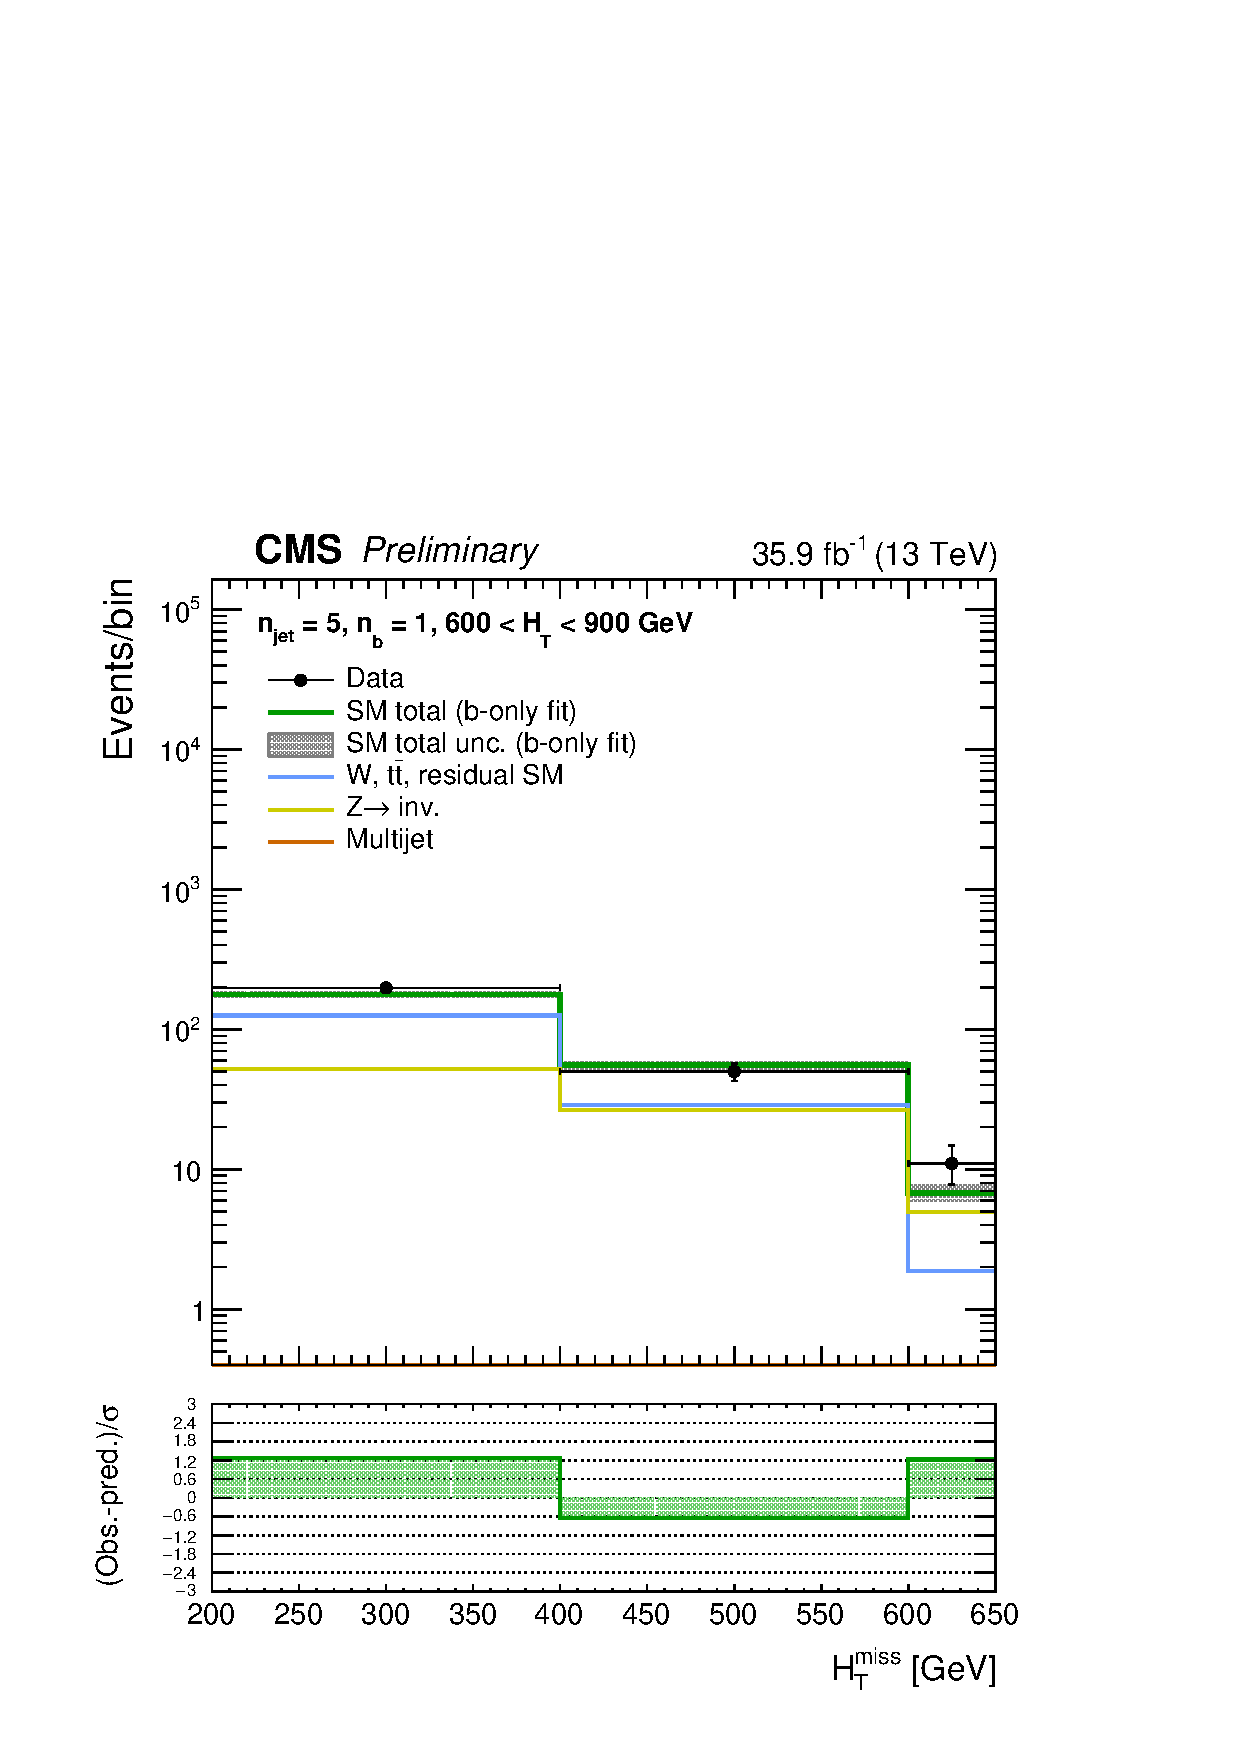
\includegraphics[width=0.49\textwidth]{figures/results/36invfb//crfit/shapes//mhtShape_eq1b_eq5j_600_900_fit_b.pdf}}\\
    \subfigure[$900 < \scalht < 1200\GeV$]{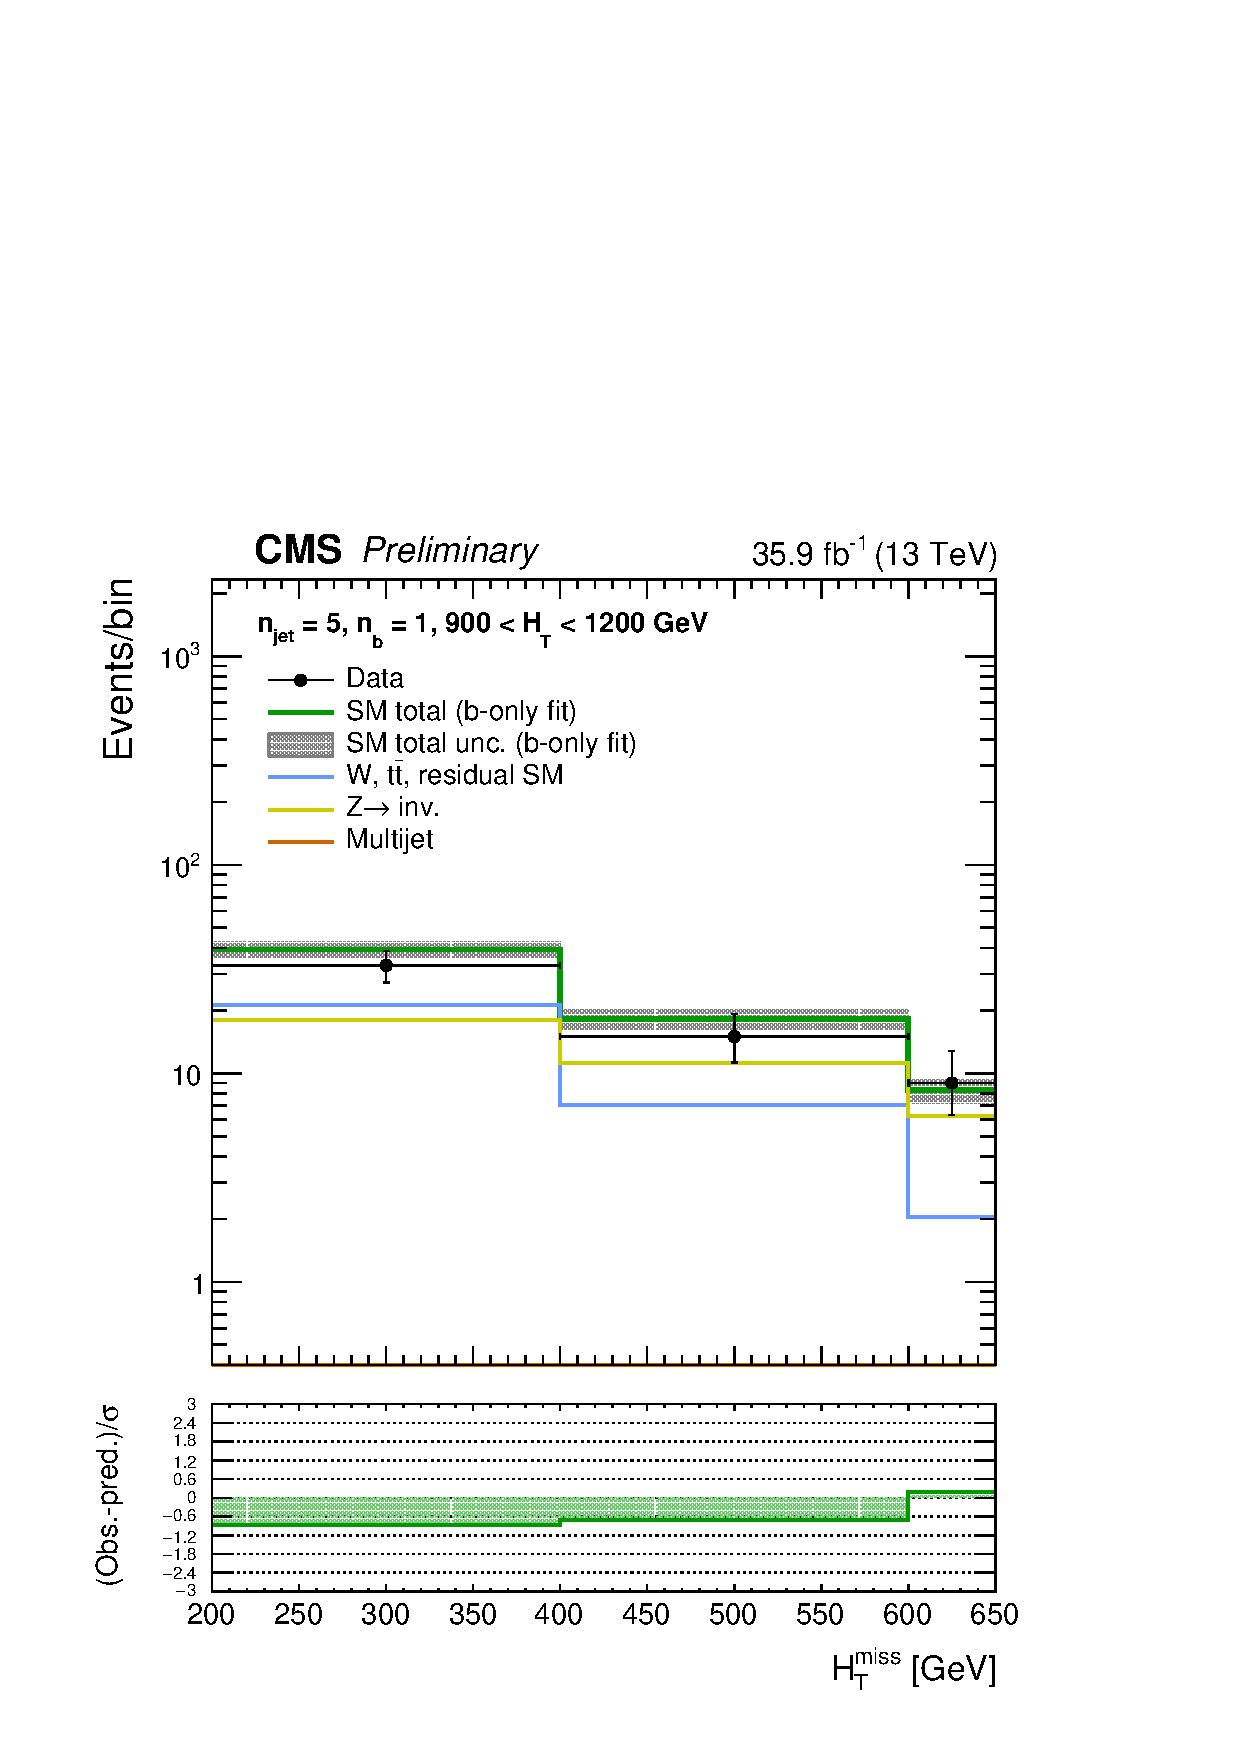
\includegraphics[width=0.49\textwidth]{figures/results/36invfb//crfit/shapes//mhtShape_eq1b_eq5j_900_1200_fit_b.pdf}}
    \subfigure[$\scalht > 1200\GeV$]{\includegraphics[width=0.49\textwidth]{figures/results/36invfb//crfit/shapes//mhtShape_eq1b_eq5j_1200_Inf_fit_b.pdf}}\\
    \caption{Event yields observed in data (solid circles) and CR-fit SM expectations with their associated uncertainties (green histogram with shaded band) as a function of \HTmiss based on a sample of events that satisfy $\njet = 5$ and $\nb = 1$, as well as the requirements on \scalht indicated by each sub-figure caption. }
    \label{fig:mhtval_eq5j_eq1b}
  \end{center}
\end{figure}

\begin{figure}[h!]
  \begin{center}
    \subfigure[$400 < \scalht < 600\GeV$]{\includegraphics[width=0.49\textwidth]{figures/results/36invfb//crfit/shapes//mhtShape_eq2b_eq5j_400_600_fit_b.pdf}}
    \subfigure[$600 < \scalht < 900\GeV$]{\includegraphics[width=0.49\textwidth]{figures/results/36invfb//crfit/shapes//mhtShape_eq2b_eq5j_600_900_fit_b.pdf}}\\
    \subfigure[$900 < \scalht < 1200\GeV$]{\includegraphics[width=0.49\textwidth]{figures/results/36invfb//crfit/shapes//mhtShape_eq2b_eq5j_900_1200_fit_b.pdf}}
    \subfigure[$\scalht > 1200\GeV$]{\includegraphics[width=0.49\textwidth]{figures/results/36invfb//crfit/shapes//mhtShape_eq2b_eq5j_1200_Inf_fit_b.pdf}}\\
    \caption{Event yields observed in data (solid circles) and CR-fit SM expectations with their associated uncertainties (green histogram with shaded band) as a function of \HTmiss based on a sample of events that satisfy $\njet = 5$ and $\nb = 2$, as well as the requirements on \scalht indicated by each sub-figure caption. }
    \label{fig:mhtval_eq5j_eq2b}
  \end{center}
\end{figure}

\begin{figure}[h!]
  \begin{center}
    \subfigure[$400 < \scalht < 600\GeV$]{\includegraphics[width=0.49\textwidth]{figures/results/36invfb//crfit/shapes//mhtShape_eq3b_eq5j_400_600_fit_b.pdf}}
    \subfigure[$600 < \scalht < 900\GeV$]{\includegraphics[width=0.49\textwidth]{figures/results/36invfb//crfit/shapes//mhtShape_eq3b_eq5j_600_900_fit_b.pdf}}\\
    \subfigure[$\scalht > 900\GeV$]{\includegraphics[width=0.49\textwidth]{figures/results/36invfb//crfit/shapes//mhtShape_eq3b_eq5j_900_Inf_fit_b.pdf}}
    \caption{Event yields observed in data (solid circles) and CR-fit SM expectations with their associated uncertainties (green histogram with shaded band) as a function of \HTmiss based on a sample of events that satisfy $\njet = 5$ and $\nb = 3$, as well as the requirements on \scalht indicated by each sub-figure caption. }
    \label{fig:mhtval_eq5j_eq3b}
  \end{center}
\end{figure}

\begin{figure}[h!]
  \begin{center}
    \subfigure[$600 < \scalht < 900\GeV$]{\includegraphics[width=0.49\textwidth]{figures/results/36invfb//crfit/shapes//mhtShape_eq0b_ge6j_600_900_fit_b.pdf}}
    \subfigure[$900 < \scalht < 1200\GeV$]{\includegraphics[width=0.49\textwidth]{figures/results/36invfb//crfit/shapes//mhtShape_eq0b_ge6j_900_1200_fit_b.pdf}}\\
    \subfigure[$\scalht > 1200\GeV$]{\includegraphics[width=0.49\textwidth]{figures/results/36invfb//crfit/shapes//mhtShape_eq0b_ge6j_1200_Inf_fit_b.pdf}}
    \caption{Event yields observed in data (solid circles) and CR-fit SM expectations with their associated uncertainties (green histogram with shaded band) as a function of \HTmiss based on a sample of events that satisfy $\njet \geq 6$ and $\nb = 0$, as well as the requirements on \scalht indicated by each sub-figure caption. }
    \label{fig:mhtval_ge6j_eq0b}
  \end{center}
\end{figure}

\begin{figure}[h!]
  \begin{center}
    \subfigure[$600 < \scalht < 900\GeV$]{\includegraphics[width=0.49\textwidth]{figures/results/36invfb//crfit/shapes//mhtShape_eq1b_ge6j_600_900_fit_b.pdf}}
    \subfigure[$900 < \scalht < 1200\GeV$]{\includegraphics[width=0.49\textwidth]{figures/results/36invfb//crfit/shapes//mhtShape_eq1b_ge6j_900_1200_fit_b.pdf}}\\
    \subfigure[$\scalht > 1200\GeV$]{\includegraphics[width=0.49\textwidth]{figures/results/36invfb//crfit/shapes//mhtShape_eq1b_ge6j_1200_Inf_fit_b.pdf}}
    \caption{Event yields observed in data (solid circles) and CR-fit SM expectations with their associated uncertainties (green histogram with shaded band) as a function of \HTmiss based on a sample of events that satisfy $\njet \geq 6$ and $\nb = 1$, as well as the requirements on \scalht indicated by each sub-figure caption. }
    \label{fig:mhtval_ge6j_eq1b}
  \end{center}
\end{figure}

\begin{figure}[h!]
  \begin{center}
    \subfigure[$600 < \scalht < 900\GeV$]{\includegraphics[width=0.49\textwidth]{figures/results/36invfb//crfit/shapes//mhtShape_eq2b_ge6j_600_900_fit_b.pdf}}
    \subfigure[$900 < \scalht < 1200\GeV$]{\includegraphics[width=0.49\textwidth]{figures/results/36invfb//crfit/shapes//mhtShape_eq2b_ge6j_900_1200_fit_b.pdf}}\\
    \subfigure[$\scalht > 1200\GeV$]{\includegraphics[width=0.49\textwidth]{figures/results/36invfb//crfit/shapes//mhtShape_eq2b_ge6j_1200_Inf_fit_b.pdf}}
    \caption{Event yields observed in data (solid circles) and CR-fit SM expectations with their associated uncertainties (green histogram with shaded band) as a function of \HTmiss based on a sample of events that satisfy $\njet \geq 6$ and $\nb = 2$, as well as the requirements on \scalht indicated by each sub-figure caption. }
    \label{fig:mhtval_ge6j_eq2b}
  \end{center}
\end{figure}

\begin{figure}[h!]
  \begin{center}
    \subfigure[$600 < \scalht < 900\GeV$]{\includegraphics[width=0.49\textwidth]{figures/results/36invfb//crfit/shapes//mhtShape_eq3b_ge6j_600_900_fit_b.pdf}}
    \subfigure[$900 < \scalht < 1200\GeV$]{\includegraphics[width=0.49\textwidth]{figures/results/36invfb//crfit/shapes//mhtShape_eq3b_ge6j_900_1200_fit_b.pdf}}\\
    \subfigure[$\scalht > 1200\GeV$]{\includegraphics[width=0.49\textwidth]{figures/results/36invfb//crfit/shapes//mhtShape_eq3b_ge6j_1200_Inf_fit_b.pdf}}
    \caption{Event yields observed in data (solid circles) and CR-fit SM expectations with their associated uncertainties (green histogram with shaded band) as a function of \HTmiss based on a sample of events that satisfy $\njet \geq 6$ and $\nb = 3$, as well as the requirements on \scalht indicated by each sub-figure caption. }
    \label{fig:mhtval_ge6j_eq3b}
  \end{center}
\end{figure}
